\documentclass[a4paper]{article}
\usepackage[T1]{fontenc}			% \chapter package
\usepackage[english]{babel}
\usepackage[english]{isodate}  		% date format
\usepackage{graphicx}				% manage images
\usepackage{amsfonts}
\usepackage{booktabs}				% high quality tables
\usepackage{amsmath}				% math package
\usepackage{amssymb}				% another math package (e.g. \nexists)
\usepackage{bm}                     % bold math symbols
\usepackage{mathtools}				% emphasize equations
\usepackage{stmaryrd} 				% '\llbracket' and '\rrbracket'
\usepackage{amsthm}					% better theorems
\usepackage{enumitem}				% manage list
\usepackage{pifont}					% nice itemize
\usepackage{cancel}					% cancel math equations
\usepackage{caption}				% custom caption
\usepackage[]{mdframed}				% box text
\usepackage{multirow}				% more lines in a table
\usepackage{textcomp, gensymb}		% degree symbol
\usepackage[x11names]{xcolor}		% RGB color
\usepackage[many]{tcolorbox}		% colorful box
\usepackage{multicol}				% more rows in a table (used for the lists)
\usepackage{listings}
\usepackage{url}
\usepackage{qrcode}
\usepackage{fontawesome5}
\usepackage{ragged2e}
\usepackage{soul}                   % highlight text (as a highlighter)
\usepackage{cite}                   % references
\usepackage{imakeidx}               % index
\makeindex[program=makeindex, columns=1,
           title=Index, 
           intoc,
           options={-s index-style.ist}]
\usepackage{fancyhdr}
\usepackage{pdflscape}   % rotates the page in the PDF viewer
\usepackage{tikz}

%\pdfcompresslevel=0
%\pdfobjcompresslevel=0

\definecolor{codegreen}{rgb}{0,0.6,0}
\definecolor{codegray}{rgb}{0.5,0.5,0.5}
\definecolor{codepurple}{rgb}{0.58,0,0.82}
\definecolor{backcolour}{rgb}{0.95,0.95,0.92}
\lstdefinestyle{mystyle}{
    backgroundcolor=\color{backcolour},
    commentstyle=\color{codegreen},
    keywordstyle=\color{magenta},
    numberstyle=\tiny\color{codegray},
    stringstyle=\color{codepurple},
    basicstyle=\ttfamily\footnotesize,
    breakatwhitespace=false,
    breaklines=true,
    captionpos=b,
    keepspaces=true,
    numbers=left,
    numbersep=5pt,
    showspaces=false,
    showstringspaces=false,
    showtabs=false,
    tabsize=2
}
\lstset{style=mystyle}


% thanks Mico: https://tex.stackexchange.com/a/60218/312896
\makeatletter
\renewcommand\paragraph{\@startsection{paragraph}{4}{\z@}%
            {-2.5ex\@plus -1ex \@minus -.25ex}%
            {1.25ex \@plus .25ex}%
            {\normalfont\normalsize\bfseries}}
\makeatother
\setcounter{secnumdepth}{4} % how many sectioning levels to assign numbers to
\setcounter{tocdepth}{4}    % how many sectioning levels to show in ToC


% draw a frame around given text
\newcommand{\framedtext}[1]{%
	\par%
	\noindent\fbox{%
		\parbox{\dimexpr\linewidth-2\fboxsep-2\fboxrule}{#1}%
	}%
}


% table of content links
\usepackage{xcolor}
\usepackage[linkcolor=black, citecolor=blue, urlcolor=cyan]{hyperref} % hypertexnames=false
\hypersetup{
	colorlinks=true
}


\newtheorem{theorem}{\textcolor{Red3}{\underline{Theorem}}}
\renewcommand{\qedsymbol}{QED}
\newcommand{\dquotes}[1]{``#1''}
\newcommand{\code}[1]{\texttt{#1}}
% I never remember every icon, so I use custom commands to do this
\newcommand{\speedIcon}{tachometer-alt}
\newcommand{\longline}{\noindent\rule{\textwidth}{0.4pt}}
\newcommand{\important}[1]{\textcolor{red}{\textbf{#1}}}
\newcommand{\circledtext}[1]{\raisebox{.5pt}{\textcircled{\raisebox{-.9pt}{#1}}}}
\newcommand{\definition}[1]{\textcolor{Red3}{\textbf{#1}}\index{#1}}
\newcommand{\example}[1]{\textcolor{Green4}{\textbf{#1}}}
\newcommand{\highspace}{\vspace{1.2em}\noindent}
\newcommand{\version}{v0.3.0}

% \includeonly{
%     sections/laboratory/introduction,
%     sections/laboratory/fem-for-poisson-1d/what-is-the-poisson-equation,
%     sections/laboratory/fem-for-poisson-1d/problem-definition,
%     sections/laboratory/fem-for-poisson-1d/weak-formulation,
%     sections/laboratory/fem-for-poisson-1d/galerkin-formulation,
%     sections/laboratory/fem-for-poisson-1d/finite-element-formulation/constructing-the-finite-element-space-vh,
%     sections/laboratory/fem-for-poisson-1d/finite-element-formulation/from-vh-to-discrete-problem,
%     sections/laboratory/fem-for-poisson-1d/implementation-in-dealii/install-and-setup,
%     sections/laboratory/fem-for-poisson-1d/implementation-in-dealii/program-structure,
%     sections/laboratory/fem-for-poisson-1d/implementation-in-dealii/general-structure,
%     sections/laboratory/fem-for-poisson-1d/implementation-in-dealii/header-file,
%     sections/laboratory/fem-for-poisson-1d/implementation-in-dealii/setup-turning-math-objects-into-dealii-objects,
%     sections/laboratory/fem-for-poisson-1d/implementation-in-dealii/assemble-compute-a-and-f,
%     sections/bibliography-and-index
% }


\begin{document}
    \newcounter{definition}[section]
    \newcounter{example}[section]
    \newcounter{exercise}[section]
    \newcounter{remark}[section]
    
    \newtcolorbox[use counter = definition]{definitionbox}[1][]{%
        breakable,
        enhanced,
        colback=red!5!white,
        colframe=red!75!black,
        fonttitle=\bfseries,
        title={Definition \thetcbcounter#1} %
    }

    \newtcolorbox[use counter = exercise]{exercisebox}[1][]{%
        breakable,
        enhanced,
        colback=Red3!5!white,
        colframe=Red3!75!black,
        fonttitle=\bfseries,
        title={Exercise \thetcbcounter#1} %
    }
    
    \newtcolorbox[use counter = example]{examplebox}[1][]{%
        breakable,
        enhanced,
        colback=Green4!5!white,
        colframe=Green4!75!black,
        fonttitle=\bfseries,
        title={Example \thetcbcounter#1} %
    }

    \newtcolorbox[use counter = remark]{remarkbox}[1][]{%
      breakable,
      enhanced,
      colback=blue!5!white,
      colframe=blue!75!black,
      fonttitle=\bfseries,
      title={Remark \thetcbcounter #1} %
    }

    \newtcolorbox[]{deepeningbox}[1][]{%
        breakable,
        enhanced,
        colback=DarkOrange3!5!white,
        colframe=DarkOrange3!75!black,
        fonttitle=\bfseries,
        title={Deepening#1} %
    }

    %%%%%%%%%%%%%%%
    % Notes cover %
    %%%%%%%%%%%%%%%
    \author{260236}
\title{Quantum Computing - Notes - \version}
\date{\printdayoff\today}
\maketitle

    %%%%%%%%%%%
    % Preface %
    %%%%%%%%%%%
	\section*{Preface}

Every theory section in these notes has been taken from two sources:
\begin{itemize}
    \item Ian Goodfellow and Yoshua Bengio and Aaron Courville, \href{https://www.deeplearningbook.org/}{Deep Learning}, MIT Press. \cite{Goodfellow-et-al-2016}
    \item Course slides.\cite{course-slides-polimi}
\end{itemize}
About:
\begin{itemize}
    \item[\faIcon{github}] \href{https://github.com/PoliMI-HPC-E-notes-projects-AndreVale69/HPC-E-PoliMI-university-notes}{GitHub repository}
    \begin{center}
        \qrcode{https://github.com/PoliMI-HPC-E-notes-projects-AndreVale69/HPC-E-PoliMI-university-notes}
    \end{center}
\end{itemize}
These notes are an unofficial resource and shouldn't replace the course material or any other book on artificial neural networks and deep learning. It is not made for commercial purposes. I've made the following notes to help me improve my knowledge and maybe it can be helpful for everyone.

As I have highlighted, a student should choose the teacher's material or a book on the topic. These notes can only be a helpful material.

\highspace
During the Artificial Neural Networks and Deep Learning course, me and my other three colleagues Alberto Ondei, \href{https://it.linkedin.com/in/javedabdullah}{Abdullah Javed} and \href{https://www.hpc.cineca.it/staff/barbari-filippo/}{Filippo Barbari}, we created two projects:
\begin{itemize}
    \item[\faIcon{github}] \href{https://github.com/PoliMI-HPC-E-notes-projects-AndreVale69/AN2DL-Challenge-1}{Time Series Classification}. Deep Neural Netowrk (TCN $+$ BiLSTM with Attention) model on multivariate time-series classification.
    \begin{center}
        \qrcode{https://github.com/PoliMI-HPC-E-notes-projects-AndreVale69/AN2DL-Challenge-1}
    \end{center}
    \item[\faIcon{github}] \href{https://github.com/PoliMI-HPC-E-notes-projects-AndreVale69/AN2DL-Challenge-2}{Image Classification}. Histopathology image classification to predict molecular subtypes.
    \begin{center}
        \qrcode{https://github.com/PoliMI-HPC-E-notes-projects-AndreVale69/AN2DL-Challenge-2}
    \end{center}
\end{itemize}

    %%%%%%%%%%%%%%%%%%%%%
    % Table of contents %
    %%%%%%%%%%%%%%%%%%%%%
    \tableofcontents
    \newpage

    %%%%%%%%%%%%%%%%%%%
    % Fancy pagestyle %
    %%%%%%%%%%%%%%%%%%%
    \pagestyle{fancy}
    \fancyhead{} % clear all header fields
    \fancyhead[R]{\nouppercase{\leftmark\hfill\rightmark}}

    %%%%%%%%%%%%%%%%%%
    % Basic Concepts %
    %%%%%%%%%%%%%%%%%%
    \section{Basic Concepts}

In this course, we introduce numerical methods for the solution of \textbf{Partial Differential Equations} (PDEs), with focus on the \textbf{Finite Element} (FE) \textbf{method}\footnote{The \definition{Finite Element Method (FEM)}\label{definition: Finite Element Method (FEM)} is a popular method for numerically solving differential equations arising in engineering and mathematical modeling. Typical problem areas of interest include the traditional fields of structural analysis, heat transfer, fluid flow, mass transport, and electromagnetic potential. Computers are usually used to perform the calculations required. With high-speed supercomputers, better solutions can be achieved, and are often required to solve the largest and most complex problems. (\href{https://en.wikipedia.org/wiki/Finite_element_method}{source})} and the use of the computer for the construction of the PDEs numerical solution.

\highspace
We will consider the numerical approximation of elliptic and parabolic PDEs by considering their variational formulation, Galërkin and FE approximations in 1D/2D/3D, the theoretical properties and practical use of the methods, algorithmic aspects, and interpretation of the numerical results.

\highspace
Advanced topics include the approximation of saddle-point PDEs (Stokes equations), vectorial, nonlinear, and multiphysics differential problems, domain decomposition methods exploiting the properties of the PDEs, and the introduction to parallel computing for the FE method, i.e., in the \emph{High Performance Computing} (HPC) framework.

\highspace
Finally, the course will feature the use of the \href{https://www.dealii.org/}{\texttt{deal.II} software library}, a C++ open source FE library, and \href{https://www.paraview.org/}{ParaView} for the visualization of numerical solution and scientific computing data.

\newpage

\subsection{Mathematical Models and Scientific Computing}

\begin{definitionbox}[: Mathematical Model]
    A \definition{Mathematical Model} is a \textbf{set of} (algebraic or differential) \textbf{equations that is able to represent the features of a complex system or process}.

    \begin{flushleft}
        \textcolor{Green3}{\faIcon{question-circle} \textbf{Why do they exist?}}
    \end{flushleft}
    Models are \textbf{developed} to:
    \begin{itemize}
        \item Describe
        \item Forecast
        \item Control
    \end{itemize}
    The \textbf{behavior or evolution of such systems}.
\end{definitionbox}

\highspace
We are interested in the physics models. \textbf{Physics-based models} are those \textbf{mathematical models that are derived from physical principles} (like conservation laws of mass, momentum, energy, etc.) \textbf{and that encode natural laws of leading to (differential) equations whose solutions are often represented in the form of functions}. However, the analytical solution of such models is rarely available in closed form, for which numerical approximation methods are instead employed.

\highspace
\begin{definitionbox}[: Numerical Modelling]
    \definition{Numerical Modelling} indicates \textbf{sets of numerical methods that determine an approximate solution of the original} (often infinite-dimensional) \textbf{mathematical model}, by turing it into a \emph{discrete problem} (algebraic, finite-dimensional), whose dimension (size) is typically very large.
\end{definitionbox}

\highspace
\begin{definitionbox}[: Scientific Computing]
    \definition{Scientific Computing} is \textbf{a branch} of Mathematics \textbf{that numerically solves} (differential) \textbf{mathematical models by building approximate solutions though the use of a calculator}.
\end{definitionbox}

\highspace
For numerical models of large size, parallel architectures for calculators and the HPC framework are typically used.

\newpage

\begin{flushleft}
    \textcolor{Green3}{\faIcon{question-circle} \textbf{Why did we introduce mathematical models and physical models?}}
\end{flushleft}
Because they are connected and used together. Mathematical models are conventionally used altogether with theoretical (mathematical) models and experimental tests. Unfortunately, in several cases theoretical models are not available (like in Computational Medicine) or experimental tests are not meaningful or cannot be performed (for example, for nuclear testing). Physics-based models have witnessed an increasing role in the modern society in virtue of the massive developments of Scientific Computing and computational tools.

\highspace
Since a large amount of data is becoming available from multiple sources nowadays, data-driven models are fundamentals. \textbf{Data-driven models} are those mathematical models built from meaningful data that do not rely on physical principles, because the latter are not available or are not reliable, and whose construction calls for statical learning methods.

\highspace
Physics-based mathematical models (\textbf{mathematical problems}) are a fundamental pillar in the understanding and prediction of several physical phenomena and processes (\textbf{physical problems}). However, these mathematical models lead to problems that can rarely be solved analytically, or in an exact way (\textbf{exact solution}), especially for PDEs: with only a few exceptions, it is not possible to write their solution explicitly.

\highspace
Numerical methods and numerical approximation techniques (\textbf{numerical problems}) serve the purpose to determine an \textbf{approximate solution} of a mathematical model. When the calculator is used to determine such approximate solution, the latter is called \textbf{numerical solution} (see the Figure \ref{fig: scientific computing}).

\begin{figure}[!htp]
    \centering
    \includegraphics[width=\textwidth]{img/models-1.pdf}
    \caption{Scientific Computing.}
    \label{fig: scientific computing}
\end{figure}
    \subsection{Differential Models and PDEs}

\begin{definitionbox}[: Partial Differential Equation (PDE)]
    A \textbf{differential equation} (model) is an equation that involves \textbf{one or more derivatives of an unknown function}. In an \textbf{Ordinary Differential Equation} (ODE), \textbf{every derivative of the unknown solution is with respect to a single independent variable}. If instead, derivatives are partial, then we have a \definition{Partial Differential Equation (PDE)}.
\end{definitionbox}

\noindent
In other words, it is a differential equation where its derivatives are partial.

\highspace
There are different types of PDEs, and their nature depends on the conditions and their type. Mathematically, we can represent a \textbf{differential model} (equation) as follows:
\begin{equation}
    \mathcal{P}\left(u; g\right) = 0 \hspace{2em} \text{differential equation (mathematical problem)}
\end{equation}
Where:
\begin{itemize}
    \item $\mathcal{P}$ indicates the \emph{\textbf{model}};
    \item $u$ is the \emph{\textbf{exact solution}}, a function of one or more independent variables (space and/or time variables);
    \item $g$ indicates the \emph{\textbf{data}}.
\end{itemize}

\highspace
\begin{deepeningbox}[: PDE]
    A \textbf{Partial Differential Equation} is the mathematical language used to describe how \textbf{continuous physical quantities} (temperature, velocity, pressure, stress, concentration, electromagnetic field, etc.) evolve in \textbf{space and time}. They express: conservation laws (mass, momentum, energy), constitutive relations (material response), and external influences (forces, sources, boundaries). \textbf{Everything around us is governed by PDEs}:
    \begin{itemize}
        \item \textbf{Physics}: Maxwell's equations (electromagnetism), Schrödinger equation (quantum mechanics), Navier-Stokes equations (fluid dynamics).
        \item \textbf{Engineering}: Heat equation (thermal analysis), wave equation (vibrations, acoustics), elasticity equations (structural mechanics).
        \item \textbf{Biology}: Reaction-diffusion equations (pattern formation, population dynamics), diffusion equations (spread of substances).
        \item \textbf{Finance}: Black-Scholes equation (option pricing).
    \end{itemize}
    They are the \textbf{continuous models of reality}.

    \highspace
    \textcolor{Green3}{\faIcon{question-circle} \textbf{Why discretization of PDEs?}} Analytic solutions exist only for simple geometries or constant coefficients. Most real-world problems, like airflow around a car, stress in a bridge, or temperature in a turbine, are too complex. So we \textbf{discretize} the PDE to convert it into a \textbf{finite-dimensional algebraic system} that we can solve numerically:
    \begin{equation*}
        A u_{h} = b
    \end{equation*}
    That's the bridge from \textbf{physics} to \textbf{mathematics} to \textbf{computation}. Discretization (via FEM, FDM, FVM, etc.) transforms ``infinitely many unknowns'' into a \textbf{finite but huge system} that captures the essential physics at chosen resolution.

    \highspace
    \textcolor{Green3}{\faIcon{question-circle} \textbf{Why solve PDEs numerically? (the \emph{purpose})}} Because solving PDEs means \textbf{simulating the real-world without physically building it}. Instead of running an expensive or dangerous experiment, we compute the solution on a computer. Some examples:
    \begin{itemize}
        \item \textbf{Aerospace}: Simulate airflow over a new aircraft design to optimize aerodynamics before building prototypes.
        \item \textbf{Climate Science}: Model global climate systems to predict future climate change scenarios.
        \item \textbf{Biomedical Engineering}: Simulate blood flow in arteries to design medical devices.
        \item \textbf{Automotive}: Crash simulations to improve vehicle safety features.
        \item \textbf{Energy}: Model heat transfer in nuclear reactors for safety analysis.
    \end{itemize}
    Every time we \textbf{discretize and solve a PDE}, we create a \textbf{digital experiment}.
\end{deepeningbox}

\newpage

\subsubsection{ODEs}

\definition{Ordinary Differential Equation (ODE)} is also known as \textbf{initial value problem}.\index{Initial value problem}

\highspace
\begin{flushleft}
    \textcolor{Green3}{\faIcon{book} \textbf{I\textdegree ODE - Cauchy problem}}
\end{flushleft}
A \textbf{first order} ODE, a \textbf{Cauchy problem}, is a differential problem, whose:
\begin{itemize}
    \item \textbf{\emph{Solution}} $u = u\left(t\right)$ is a function of a single independent variable $t$, often interpreted as time.
    \item A \textbf{\emph{single condition}} is assigned on the solution, at a point (usually, the left end of the integration interval).
\end{itemize}
Its form is the following find $u : I \subset \mathbb{R} \rightarrow \mathbb{R}$ such that:
\begin{equation}
    \begin{cases}
        \dfrac{\mathrm{d}u}{\mathrm{d}t}\left(t\right) = f\left(t, u\left(t\right)\right) & t \in I \vspace{1em} \\
        u\left(t_{0}\right) = u_{0}
    \end{cases}
\end{equation}
Where:
\begin{itemize}
    \item $I = \left( t_{0}, t_{f} \right] \subset \mathbb{R}$ is a \emph{\textbf{time interval}};
    \item $u_{0}$ is the \emph{\textbf{initial value}} assigned at $t = t_{0}$;
    \item $f: I \times \mathbb{R} \rightarrow \mathbb{R}$
\end{itemize}
\textcolor{Green3}{\faIcon{question-circle} \textbf{Meaning}}. The equation describes the \textbf{evolution of a scalar quantity $u$ over time $t$}, \textbf{without distribution in space}.

\highspace
\textcolor{Green3}{\faIcon{question-circle} \textbf{Vectorial problems}}. In vectorial problems, the \textbf{unknown is a vector-valued function} $\mathbf{u} = \mathbf{u}\left(t\right)$, where $\mathbf{u} = \left(u_{1}, \dots, u_{m}\right) \in \mathbb{R}^{m}$, with $m \ge 1$. The first order Cauchy problem reads: find $\mathbf{u} : I \subset \mathbb{R} \rightarrow \mathbb{R}^{m}$ such that:
\begin{equation*}
    \begin{cases}
        \dfrac{\mathrm{d}\mathbf{u}}{\mathrm{d}t}\left(t\right) = \mathbf{f}\left(t, \mathbf{u}\left(t\right)\right) & t \in I \vspace{1em} \\
        \mathbf{u}\left(t_{0}\right) = \mathbf{u}_{0}
    \end{cases}
\end{equation*}
Where $\mathbf{u}_{0} \in \mathbb{R}^{m}$ is the initial datum and $\mathbf{f}: I \times \mathbb{R}^{m} \rightarrow \mathbb{R}^{m}$.

\highspace
\begin{flushleft}
    \textcolor{Green3}{\faIcon{book} \textbf{II\textdegree ODE - Cauchy problem}}
\end{flushleft}
A \textbf{second order Cauchy problem} sees second order time derivatives and two initial conditions. It reads as: find $u: I \subset \mathbb{R} \rightarrow \mathbb{R}$ such that:
\begin{equation}
    \begin{cases}
        \dfrac{\mathrm{d}^{2}u}{\mathrm{d}t^{2}}\left(t\right) = f\left(t, u\left(t\right), \dfrac{\mathrm{d}u}{\mathrm{d}t}\left(t\right)\right) & t \in I \vspace{1em} \\
        \dfrac{\mathrm{d}u}{\mathrm{d}t}\left(t_{0}\right) = v_{0} \vspace{1em} \\
        u\left(t_{0}\right) = u_{0}
    \end{cases}
\end{equation}
Where the initial data are $u_{0}$ and $v_{0}$, while $f: I \times \mathbb{R} \times \mathbb{R} \rightarrow \mathbb{R}$.
    \subsubsection{PDE, boundary value problem in 1D}

The \definition{Boundary value problem in 1D} is characterized by a \textbf{single independent variable} $x$, which represents the \textbf{space coordinate in an interval} $\Omega = \left(a,b\right) \in \mathbb{R}$ (1D).

\highspace
The problem involves \textbf{second order derivatives of the unknown solution} $u = u\left(x\right)$ with respect to $x$. The value of $u$, or the \textbf{value of its first derivate}, is a \textbf{set at the two boundaries of the domain} (interval) $\Omega$, that is at $x = a$ and $x = b$ (the domain boundary is $\partial\Omega = \left\{a,b\right\})$.

\highspace
Let us consider the following Poisson problem with (homogeneous) Dirichlet boundary conditions: find $u : \Omega \subset \mathbb{R} \rightarrow \mathbb{R}$ such that:
\begin{equation}
    \begin{cases}
        -\dfrac{\mathrm{d}^{2}u}{\mathrm{d}x^{2}}\left(x\right) = f\left(x\right) & x \in \Omega = \left(a,b\right) \vspace{1em} \\
        %
        u\left(a\right) = u\left(b\right) = 0
    \end{cases}
\end{equation}
This equation models a \textbf{stationary phenomenon} (the time variable doesn't appear in fact) and represent a \textbf{diffusion model}.

\highspace
\begin{examplebox}
    For example, the diffusion model models the diffusion of a pollutant along a 1D channel $\Omega = \left(a,b\right)$ or the vertical displacement of an \emph{elastic thread} fixed at its ends. In the first case, $f = f\left(x\right)$ indicates the source of the pollutant along the flow, while in the second case, $f$ is the traverse force acting on the elastic thread, in the hypothesis of negligible mass and small displacements of the thread.
\end{examplebox}

\noindent
\begin{flushleft}
    \textcolor{Green3}{\faIcon{balance-scale} \textbf{Boundary value problem in 1D vs ODE}}
\end{flushleft}
We remark that the \textbf{boundary value problem in 1D is a particular case of PDEs}, even if it involves only derivatives with respect to a single independent variable $x$. Indeed, even if apparently similar to a second order ODE, the boundary value problem is in reality substantially \textbf{different} from an ODE:
\begin{itemize}
    \item In ODE, two conditions are set at $t = t_{0}$;
    \item In the boundary value problem in 1D, one condition is set at $x = a$ and the other one at $x = b$.
\end{itemize}
The conditions in the boundary value problem determine to the so-called global nature of the model.
    \subsubsection{PDE, initial and boundary value problem in 1D}

\definition{Initial and boundary value problem in 1D} is a type of problems that concern equations that \textbf{depend on space and time}:
\begin{itemize}
    \item The \textbf{unknown solution} $u = u\left(x,t\right)$ both depends on the space coordinate $x \in \Omega \subset \mathbb{R}$ in 1D;
    
    \item The \textbf{time variable} $t \in I \subset I$.
\end{itemize}
In this case, the initial conditions at $t = 0$ must be prescribed, as well as the boundary conditions at the ends of the interval in 1D.

\highspace
The \definition{Heat equation}, also known as \definition{Diffusion equation}, with Dirichlet boundary conditions assumes the following form: find $u: \Omega \times I \rightarrow \mathbb{R}$ such that:
\begin{equation}
    \begin{cases}
        \dfrac{\partial u}{\partial t}\left(x,t\right) - \mu \dfrac{\partial^{2}u}{\partial x^{2}}\left(x,t\right) = f\left(x,t\right) & x \in \Omega = \left(a,b\right), t \in I \vspace{1em} \\
        %
        u\left(a,t\right) = u\left(b,t\right) = 0 & t \in I \\
        %
        u\left(x, t_{0}\right) = u_{0}\left(x\right) & x \in \Omega = \left(a,b\right)
    \end{cases}
\end{equation}

\begin{examplebox}
    For example, the unknown function $u \left(x,t\right)$ describes the temperature in a point $x \in \Omega = \left(a,b\right)$ and time $t \in I$ of a metallic bar covering the space interval $\Omega$. The diffusion coefficient $\mu$ represents the thermal response of the material and it is related to its thermal conductivity. The Dirichlet boundary conditions express the fact that the ends of the bar are kept at a reference temperature (zero degrees in this case), while at time $t = t_{0}$ the temperature is assigned in each point $x \in \Omega$ through the initial function $u_{0}\left(x\right)$. Finally, the bar is subject to a heat source of linear density $f\left(x,t\right)$.
\end{examplebox}
    \subsubsection{PDE, boundary value problem in multidimensional domains}

The Poisson problem (equation \ref{eq: Poisson problem}, page \pageref{eq: Poisson problem}) can be \textbf{extended in multidimensional domains} $\Omega \subset \mathbb{R}^{d}$, with $d = 2, 3$; the solution is $u = u\left(\mathbf{x}\right)$, where $\mathbf{x} = \left(x_{1}, \dots, x_{d}\right)^{T} \in \mathbb{R}^{d}$. This leads to the following Poisson problem with (homogeneous) Dirichlet boundary conditions: find $u: \Omega \subset \mathbb{R}^{d} \rightarrow \mathbb{R}$ such that:
\begin{equation}
    \begin{cases}
        -\Delta u = f   & \text{in } \Omega \: \left(\text{i.e. } \mathbf{x} \in \Omega\right) \\
        u = 0           & \text{on } \partial\Omega \: \left(\text{i.e. } \mathbf{x} \in \partial\Omega\right)
    \end{cases}
\end{equation}
Where:
\begin{itemize}
    \item The \definition{Laplace operator}:
    \begin{equation*}
        \Delta u \left(\mathbf{x}\right) := \displaystyle\sum_{i=1}^{d} \dfrac{\partial^{2} u}{\partial x_{i}^{2}}\left(\mathbf{x}\right)
    \end{equation*}

    \item The \textbf{domain} $\Omega \subset \mathbb{R}^{d}$ is endowed with boundary $\partial \Omega$;

    \item $f = f\left(x\right)$ is the \emph{\textbf{external forcing term}}.
\end{itemize}
This equation is used \example{for example} to \textbf{model the vertical displacement of an elastic membrane fixed at the boundaries}.

\longline

\subsubsection{PDE, initial and boundary value problem in multidimensional domains}

The \textbf{multidimensional} counterpart of the \textbf{heat equation} (\ref{eq: heat equation}, page \pageref{eq: heat equation}) reads: find $u : \Omega \times I \rightarrow \mathbb{R}$ such that:
\begin{equation}\index{Multidimensional Heat equation}
    \begin{cases}
        \dfrac{\partial u}{\partial t} - \mu\Delta u = f & \mathbf{x} \in \Omega, t \in I \vspace{1em} \\
        %
        u\left(\mathbf{x}, t\right) = 0 & \mathbf{x} \in \partial\Omega, t \in I \\
        %
        u\left(\mathbf{x}, t_{0}\right) = u_{0}\left(\mathbf{x}\right) & \mathbf{x} \in \Omega
    \end{cases}
\end{equation}
Where $u_{0}$ is the \textbf{initial datum}. The \textbf{solution} is $u = u\left(\mathbf{x}, t\right)$.
    \subsubsection{Classification of PDEs}

A PDE is a relationship among:
\begin{itemize}
    \item The partial derivatives of a function $u = u\left(\mathbf{u}, t\right)$, that is the PDE \textbf{solution};
    \item \textbf{Spatial coordinates} $\mathbf{x} = \left(x_{1}, \dots, x_{d}\right)^{T} \in \mathbb{R}^{d}$ on which the solution depends (if the problem is defined in a spatial domain $\Omega \subset \mathbb{R}^{d}$).
    \item \textbf{Time variable} $t$.
\end{itemize}
Therefore, a PDE can be written as:
\begin{equation}
    \mathcal{P}\left(
        u,
        \dfrac{\partial u}{\partial t},
        \dfrac{\partial u}{\partial x_{1}},
        \dots,
        \dfrac{\partial u}{\partial x_{d}},
        \dots,
        \dfrac{\partial^{p_{1} + \dots + p_{d} + p_{t}} u}{\partial x_{1}^{p_{1}} \dots \partial x_{d}^{p_{d}} \: \partial t^{p_{t}}},
        \mathbf{x},
        t;
        g
    \right) = 0
\end{equation}
Where $p_{1}, \dots, p_{d}, p_{t} \in \mathbb{N}$ and $g$ are the data.

\highspace
\begin{definitionbox}[: PDE order]
    The \definition{PDE order} is the \textbf{maximum order of derivation} that appears in $\mathcal{P}$, that is:
    \begin{equation}
        q = p_{1} + \dots + p_{d} + p_{t}
    \end{equation}
\end{definitionbox}

\begin{definitionbox}[: PDE is linear]
    The \definition{PDE is linear} if $\mathcal{P}$ \textbf{linearly depends} on $u$ and its \textbf{derivatives}.
\end{definitionbox}

\highspace
\begin{flushleft}
    \textcolor{Green3}{\faIcon{square-root-alt} \textbf{Classification}}
\end{flushleft}
Let us focus on linear PDEs of order $q = 2$ with constant coefficients, so that the general PDE formulation is:
\begin{equation*}
    \mathcal{L}u = g
\end{equation*}
Where $\mathcal{L}$ is a second order, \textbf{linear differential operator}. When only two independent variables (our case) $x_{1}$ and $x_{2}$ are considered, the operator $\mathcal{L}$ applied to the function $u$ reads:
\begin{equation*}
    \mathcal{L}u = 
    A \cdot \dfrac{\partial^{2} u}{\partial x_{1}^{2}} +
    B \cdot \dfrac{\partial^{2} u}{\partial x_{1} \: \partial x_{2}} +
    C \cdot \dfrac{\partial^{2} u}{\partial x_{2}^{2}} +
    D \cdot \dfrac{\partial u}{\partial x_{1}} +
    E \cdot \dfrac{\partial u}{\partial x_{2}} +
    F \cdot u
\end{equation*}
For some constant coefficients $A, B, C, D, E, F, G \in \mathbb{R}$. If $d = 2$ (our case), the \textbf{independent variables} can represent the \emph{space coordinates}:
\begin{itemize}
    \item $x_{1} = x$
    \item $x_{2} = y$
\end{itemize}
After introducing the \definition{PDE discriminant} (a quantity that helps determine the type of PDE):
\begin{equation}
   \Delta := B^{2} - 4AC 
\end{equation}
\newpage
\noindent
The PDE can be classified as:
\begin{itemize}
    \item \definition{Elliptic PDE} if $\Delta < 0$
    \item \definition{Parabolic PDE} if $\Delta = 0$
    \item \definition{Hyperbolic PDE} if $\Delta > 0$
\end{itemize}

\begin{flushleft}
    \textcolor{Green3}{\faIcon{question-circle} \textbf{What are the implications of PDE classification?}}
\end{flushleft}
The different nature of the PDE impacts on:
\begin{itemize}
    \item \textbf{Type} and \textbf{amount of data to prescribe as boundary};
    \item \textbf{Initial conditions} to ensure the well-posedness of the problem (existence and uniqueness of the solution);
    \item The \textbf{phenomena that can be described} by the PDE;
    \item The \textbf{information that encapsulates}.
\end{itemize}
In general:
\begin{itemize}
    \item \textbf{Elliptic PDE} typically describes \textbf{stationary phenomena}, without time evolution of quantities.
    \item \textbf{Parabolic PDE} describes \textbf{wave propagation phenomena} with \underline{infinite} velocity of propagation.
    \item \textbf{Hyperbolic PDE} describes \textbf{wave propagation phenomena} but with \underline{finite} velocity of propagation.
\end{itemize}
    \subsection{Numerical Methods}

Since in most cases of practical interest we \textbf{cannot solve a PDE analytically}, we need to use \textbf{numerical methods} that allow us to construct an \emph{approximation} $u_{h}$ of the \emph{exact solution} $u$, for which the corresponding \emph{error} $\left(u - u_{h}\right)$ can be quantified and/or estimated.
\begin{equation*}
    \begin{array}{cc}
        \mathcal{P}\left(u; g\right) = 0 \hspace{1em} & \text{PDE (mathematical problem)} \\ [.3em]
        \downarrow \hspace{1em} & \emph{numerical method} \\ [.3em]
        \mathcal{P}_{h}\left(u_{h}; g_{h}\right) = 0 \hspace{1em} & \text{approximate PDE (numerical problem)}
    \end{array}
\end{equation*}
Where:
\begin{itemize}
    \item $g_{h}$ is an approximation of the data $g$;
    \item $\mathcal{P}_{h}$ is a characterization of the approximate problem.
\end{itemize}
The subscript $h$ indicates a \textbf{discretization parameter} that characterizes the numerical approximation. Conventionally, the smaller is $h$, the better is the approximation of $u$ made by $u_{h}$. Furthermore, the error $\left(u - u_{h}\right)$ tends to zero as $h$ gets smaller and smaller. In this course, we will specifically introduce the FE method (page \pageref{definition: Finite Element Method (FEM)}) to build the numerical approximation of PDEs.

\highspace
\begin{flushleft}
    \textcolor{Green3}{\faIcon{bookmark} \textbf{Summary Notation}}
\end{flushleft}

\begin{table}[!htp]
    \centering
    \begin{tabular}{@{} c p{25em} @{}}
        \toprule
        \textbf{Notation} & \textbf{Description} \\
        \midrule
        $\mathcal{P}\left(u; g\right) = 0$ & PDE (mathematical problem) \\ [.5em]
        $u$ & \textbf{\emph{exact solution}} of a PDE \\ [.5em]
        $u_{h}$ & \textbf{\emph{approximate solution}} of a PDE \\ [.5em]
        $\left(u - u_{h}\right)$ & \textbf{\emph{error}} (quantified and/or estimated; tends to zero if $h$ is smaller) \\ [.5em]
        $h$ & \textbf{\emph{discretization parameter}} ($\downarrow$ smaller $h$, better approximation; $\uparrow$ higher $h$, poor approximation) \\ [.5em]
        $\mathcal{P}_{h}\left(u_{h}; g_{h}\right) = 0$ & approximate PDE (numerical problem) \\ [.5em]
        $g_{h}$ & \textbf{\emph{approximation}} of the \textbf{\emph{data}} $g$ \\ [.5em]
        $\mathcal{P}_{h}$ & \textbf{\emph{characterization}} of the approximate problem. \\
        \bottomrule
    \end{tabular}
    \caption{Notation used to approximate the PDE with numerical methods.}
\end{table}
    \subsection{From Mathematical to Numerical Problem}

\subsubsection{The mathematical problem}

Let us consider a \definition{Physical Problem (PP)} endowed with a \textbf{physical solution}, let say $u_{ph}$, and \textbf{dependent on data} indicated with $g$.

\highspace
The \definition{Mathematical Problem (MP)} is represented by the \textbf{mathematical formulation of the PP} and has \textbf{mathematical solution} $u$. Therefore, we indicate the MP as:
\begin{equation}\label{eq: mathematical problem}
    \mathcal{P}\left(u; g\right) = 0
\end{equation}
Where:
\begin{itemize}
    \item $u \in \mathcal{U}$
    \item $g \in \mathcal{G}$, and $\mathcal{G}$ is the set or space of \textbf{admissible data}.
\end{itemize}
Where $\mathcal{U}$ and $\mathcal{G}$ are suitable sets or spaces.

\highspace
\begin{definitionbox}[: Model Error]
    The error between the physical and mathematical solutions is called \definition{Model Error}:
    \begin{equation}
        e_{m} := u_{ph} - u
    \end{equation}
    Where:
    \begin{itemize}
        \item $u_{ph}$ is the physical solution;
        \item $u$ is the mathematical solution.
    \end{itemize}
\end{definitionbox}

\noindent
The model error takes into account all those \textbf{characteristics of the PP that are not represented or captured by the MP}.

\highspace
\begin{flushleft}
    \textcolor{Green3}{\faIcon{question-circle} \textbf{When a Mathematical Problem is \emph{well-posed}?}}
\end{flushleft}
\begin{definitionbox}[: well-posed MP]
    The mathematical problem MP is \emph{well-posed} (\textbf{stable}) if and only if there \textbf{exists a unique solution} $u \in \mathcal{U}$ \textbf{that continuously depend on the data} $g \in \mathcal{G}$.
\end{definitionbox}

\noindent
From the previous definition, we remark that $\mathcal{G}$ is the set of admissible data, i.e., those for which the MP admits a unique solution. Furthermore, \emph{continuously depend on the data} means that \textbf{small perturbations on data} $g \in \mathcal{G}$ \textbf{lead to small changes on the solution} $u \in \mathcal{U}$ of the MP. However, a measure of this sensitivity is given by the condition number of the MP.
    \subsubsection{The Numerical Problem (NP)}

The \definition{Numerical Problem (NP)} is an \textbf{approximation of the Mathematical Problem} (MP, equation \ref{eq: mathematical problem (MP)}, page \pageref{eq: mathematical problem (MP)}). We indicate its \textbf{numerical solution} as $u_{h}$, where $h$ stands as a suitable \textbf{discretization parameter}.
\begin{equation}\label{eq: numerical problem (NP)}
    \mathcal{P}_{h}\left(u_{h}; g_{h}\right) = 0
\end{equation}
Where:
\begin{itemize}
    \item $u_{h} \in \mathcal{U}_{h}$
    \item $g_{h} \in \mathcal{G}_{h}$, and $g_{h}$ is the representation of the \textbf{data in the NP}.
\end{itemize}
Where $\mathcal{U}_{h}$ and $\mathcal{G}_{h}$ are suitable sets or spaces.

\highspace
\begin{definitionbox}[: Truncation Error]
    The error between the mathematical and numerical solutions is called \definition{Truncation Error}:
    \begin{equation}\label{eq: Truncation Error}
        e_{h} := u - u_{h}
    \end{equation}
    Where:
    \begin{itemize}
        \item $u$ is the mathematical solution;
        \item $u_{h}$ is the numerical solution.
    \end{itemize}
\end{definitionbox}

\noindent
The truncation error can be considered as the error resulting from the \textbf{discretization of the MP}.

\highspace
\begin{flushleft}
    \textcolor{Green3}{\faIcon{laptop-code} \textbf{Numerical solution calculated on the computer}}
\end{flushleft}
When the numerical solution is computed by running the algorithm on a computer, we need more notations and concepts.
\begin{itemize}
    \item $\widehat{u}_{h}$ is the \textbf{final solution}.

    \item The final solution is affected by a \definition{Round-Off error} $e_{r}$:
    \begin{equation}\label{eq: Round-Off error}
        e_{r} := u_{h} - \widehat{u}_{h}
    \end{equation}
    Such round-off errors depend on the machine architecture, on the representation of the numbers at the calculator, and on operations made in floating-point arithmetic.

    \item The truncation error $e_{h}$ (equation \ref{eq: Truncation Error}, page \pageref{eq: Truncation Error}) and the Round-Off error $e_{r}$ (equation \ref{eq: Round-Off error}) concur to determine the \definition{Computational error} $e_{c}$:
    \begin{equation}
        e_{c} := e_{h} + e_{r} = \left(u - \cancel{u_{h}}\right) + \left(\cancel{u_{h}} - \widehat{u}_{h}\right) = u - \widehat{u}_{h}
    \end{equation}
    For some NP, we can have a round-off error less than a truncation error $\left|e_{r}\right| \ll \left|e_{h}\right|$, for which $e_{c} \approx e_{h}$.
\end{itemize}

\newpage

\begin{flushleft}
    \textcolor{Green3}{\faIcon{question-circle} \textbf{When a Numerical Problem is \emph{well-posed}?}}
\end{flushleft}
\begin{definitionbox}[: \emph{well-posed} NP]
    The numerical problem NP is \emph{well-posed} (\textbf{stable}) if and only if there \textbf{exists a unique solution} $u_{h} \in \mathcal{U}_{h}$ \textbf{that continuously depends on the data} $g_{h} \in \mathcal{G}_{h}$.
\end{definitionbox}

\highspace
\begin{flushleft}
    \textcolor{Green3}{\faIcon{laptop-code} \textbf{Consider the numerical solution calculated only on the computer}}
\end{flushleft}
In practice, numerical solutions are computed on a computer. Therefore, it is reasonable to obtain a computational error that tends to zero as the numerical method improves, namely as the discretization parameter $h$ goes to zero. This concept is encoded in the definition of convergence.

\begin{definitionbox}[: \emph{convergence} NP]
    The NP is \textbf{convergent} when the \textbf{computational error tends to zero} for $h$ tending to zero, that is:
    \begin{equation}
        \lim\limits_{h \rightarrow 0} e_{c} = 0
    \end{equation}
\end{definitionbox}

\noindent
A crucial aspect is to qualify the convergence of the NP, that is determining the convergence order of the NP.

\begin{definitionbox}[: convergence order]\index{Convergence order}
    If $\left|e_{c}\right| \le Ch^{p}$, with $C$ a positive constant independent of $h$ and $p$, then the NP is \textbf{convergent with order} $p$.
\end{definitionbox}

\highspace
\begin{flushleft}
    \textcolor{Green3}{\faIcon{question-circle} \textbf{How to estimate the convergence order?}}
\end{flushleft}
The convergence order can be estimated for many reasons (error estimation, method comparison, accuracy verification, etc.). If there exists a constant $\tilde{C} \le C$ independent of $h$ and $p$ such that $\tilde{C}h^{p} \le \left|e_{c}\right| \le C h^{p}$, then we can write $\left|e_{c}\right| \approxeq Ch^{p}$ and we can \textbf{estimate the convergence order $p$ of the NP by using the known solution $u$ of the MP}. There are two approaches:
\begin{enumerate}
    \item \textbf{Algebraic estimation} of $p$.
    \begin{enumerate}
        \item We compute the computational errors $e_{c1}$ and $e_{c2}$ for the NP corresponding to two different values of $h$ that are \dquotes{sufficietly} small, say $h_{1}$ and $h_{2}$.
        \item Then:
        \begin{itemize}
            \item Writing $\left|e_{c1}\right| \approxeq Ch_{1}^{p}$ and $\left|e_{c2}\right| \approxeq Ch_{2}^{p}$
            \item Noticing that $\dfrac{\left|e_{c1}\right|}{\left|e_{c2}\right|} = \left(\dfrac{h_{1}}{h_{2}}\right)^{p}$
        \end{itemize}
        We estimate the order $p$ as:
        \begin{equation}
            p = \dfrac{
                \log\left(\dfrac{\left|e_{c1}\right|}{\left|e_{c2}\right|}\right)
            }{
                \log\left(\dfrac{h_{1}}{h_{2}}\right)
            }
        \end{equation}
    \end{enumerate}
    
    \item \textbf{Graphical estimation} of $p$. We represent the errors $\left|e_{c}\right|$ and $h$ on a plot in log-log scale. As $\log\left|e_{c}\right| = \log\left(Ch^{p}\right) = log\left(C\right) + p \log\left(h\right)$, we have $p = \arctan\left(\theta\right)$, where $\theta$ is the slope of the curve $\left(h, e_{c}\right)$, a straight line in log-log scale. Instead of computing $\theta$, it is possible to verify that the curves $\left(h, e_{c}\right)$ and $\left(h, h^{p}\right)$ are parallel in log-log scale.

    In other words it involves plotting the error against the step size on a log-log scale and analyzing the resulting graph:
    \begin{enumerate}
        \item \emph{\textbf{Compute Errors}}: Perform the numerical method for several step sizes $h$, such as $ h_{1}, h_{2}, h_{3}, \dots $, and compute the corresponding errors $ e_{1}, e_{2}, e_{3}, \dots $.

        \item \emph{\textbf{Log-Log Plot}}: Plot the errors $e_{i}$ against the step sizes $h_{i}$ on a log-log scale. This means we plot $\log\left(h_{i}\right)$ on the x-axis and $\log\left(e_{i}\right)$ on the y-axis.

        \item \emph{\textbf{Linear Relationship}}: If the method has a convergence order $p$, the relationship between the error and the step size should follow $e \approx C h^p $. Taking the logarithm of both sides gives:
        \begin{equation*}
            \log\left(e\right) \approx \log\left(C\right) + p \log\left(h\right)
        \end{equation*}
        This indicates that the plot of $\log\left(e\right)$ versus $\log\left(h\right)$ should be a straight line with a slope equal to $p$.

        \item \emph{\textbf{Determine Slope}}: The slope of the line in the log-log plot is the convergence order $p$. We can estimate this slope by fitting a linear regression line to the data points.
    \end{enumerate}

    \begin{figure}[!htp]
        \centering
        \includegraphics[width=\textwidth]{img/graphical-estimate-1.pdf}
        \caption{Graphical estimation of the convergence order $p$ of a NP: computational errors $\left|e_{c}\right|$ vs $h$.}
    \end{figure}
\end{enumerate}

\newpage

\begin{flushleft}
    \textcolor{Green3}{\faIcon{question-circle} \textbf{When is convergence guaranteed in NP?}}
\end{flushleft}
Unfortunately, a \textbf{\emph{well-posed} NP is not necessarily convergent}. To ensure convergence of the NP, this is required to satisfy the consistency property (roughly speaking, the NP must be a \dquotes{faithful copy} of the original MP).

\highspace
\begin{definitionbox}[: NP consisten and strongly consistent]
    The Numerical Problem NP is \textbf{consistent} if and only if:
    \begin{equation*}
        \lim\limits_{h \rightarrow 0}\mathcal{P}_{h}\left(u; g\right) = \mathcal{P}\left(u;g\right) = 0 \hspace{2em} g \in \mathcal{G}_{h}
    \end{equation*}

    The Numerical Problem NP is \textbf{\emph{strongly} consistent} if and only if:
    \begin{equation*}
        \mathcal{P}_{h}\left(u; g\right) \equiv \mathcal{P}\left(u;g\right) = 0 \hspace{2em} \forall h > 0, \: g \in \mathcal{G}_{h}
    \end{equation*}
\end{definitionbox}

\highspace
Let highlights the main differences:
\begin{itemize}
    \item Definition:
    \begin{itemize}
        \item \textcolor{Green4}{\emph{\textbf{Consistent}}}. Consistency requires that as the discretization parameter \( h \) tends to zero $\lim\limits_{h \rightarrow 0}$, the process \( \mathcal{P}_{h}(u; g) \) approaches the exact process \( \mathcal{P}(u; g) \) and both become zero. This means that \textbf{over time and with finer discretization}, the \textbf{numerical approximation converges to the exact solution}.

        \item \textcolor{Green4}{\emph{\textbf{Strongly Consistent}}}. Strong consistency means that for any positive value of \( h \) ($\forall h > 0$, no matter how small), the process \( \mathcal{P}_{h}(u; g) \) is exactly equal to the exact process \( \mathcal{P}(u; g) \) and both are zero. This implies that the \textbf{numerical approximation already matches the exact solution for any step size}.
    \end{itemize}

    \item Condition of $h$:
    \begin{itemize}
        \item \textcolor{Green4}{\emph{\textbf{Consistent}}}. The condition applies in the limit as \( h \) approaches zero. The \textbf{process gradually converges to the exact solution as the discretization parameter becomes infinitesimally small}.

        \item \textcolor{Green4}{\emph{\textbf{Strongly Consistent}}}. The condition applies for all \( h > 0 \). This is a \textbf{stronger requirement} because it demands that the numerical method is \textbf{accurate for any discretization parameter}, not just in the limit.
    \end{itemize}
\end{itemize}
In practice, the \emph{Consistent} indicates that the numerical method improves and approaches the exact solution as the discretization parameter is refined. It guarantees eventual \emph{\textbf{accuracy}}, \emph{\textbf{but not necessarily immediate or uniform accuracy for larger}} \( h \). On the other hand, \emph{Strongly Consistent} indicates that the numerical method is always accurate, regardless of the discretization parameter. This implies a \emph{\textbf{higher level of reliability and precision for any}} \( h \), making it a stronger and more robust form of consistency.

\newpage

\noindent
The \definition{Lax-Richtmyer Equivalence Theorem} is a cornerstone of numerical analysis, linking the concepts of consistency, well-posedness (stability), and convergence. It provides a \textbf{rigorous framework for validating numerical methods and ensuring that they produce accurate and reliable solutions}. Furthermore, the following theorem guarantees that if a \textbf{\emph{numerical problem is well-posed and consistent, then the NP is also convergent}}.
\begin{theorem}[Lax-Richtmyer, equivalence]
    If the Numerical Problem NP:
    \begin{equation*}
        \mathcal{P}_{h}\left(u_{h}; g_{h}\right) = 0 \hspace{2em} u_{h} \in \mathcal{U}_{h}, \: g_{h} \in \mathcal{G}_{h}
    \end{equation*}
    Is consistent:
    \begin{equation*}
        \lim\limits_{h \rightarrow 0}\mathcal{P}_{h}\left(u; g\right) = \mathcal{P}\left(u;g\right) = 0 \hspace{2em} g \in \mathcal{G}_{h}
    \end{equation*}
    Then, it is well-posed if and only if it is also convergent.
\end{theorem}

\noindent
It is a fundamental theorem in numerical analysis because \textbf{it ensures that stability and consistency are sufficient to guarantee convergence}. Conversely, if we have a proof that the NP is consistent, we \dquotes{only} need to show that the problem is well-posed to automatically prove convergence (and vice versa).

\highspace
\begin{figure}[!htp]
    \centering
    \includegraphics[width=\textwidth]{img/pp-mp-np-1.pdf}
    \caption{Physical (PP), Mathematical (MP), and Numerical (NP) problems. Corresponding solutions $\left(u_{ph}, u, u_{h}, \text{ and } \widehat{u}_{h}\right)$ and errors (model $e_{m} = u_{ph} - u$, truncation $e_{h} = u - u_{h}$, round-off $e_{r} = u_{h} - \widehat{u}_{h}$, and computational $e_{c} = e_{h} + e_{r}$ errors).}
    \label{fig: PP, MP and NP}
\end{figure}

    %%%%%%%%%%%%%%
    % Laboratory %
    %%%%%%%%%%%%%%
    \section{VLIW (Very Long Instruction Word)}

\subsection{Introduction}

Traditional \textbf{compilers} use \textbf{static code scheduling} to exploit Instruction-Level Parallelism (ILP). Key tasks of the compiler:
\begin{itemize}
    \item  Detect \textbf{parallelizable} instructions considering: Hardware resource constraints and Data dependencies.
    \item \textbf{Schedule} instructions to execute \textbf{in parallel} when possible.
    \item Otherwise, \textbf{insert \texttt{NOP}s} (No Operations) if no safe parallel execution is possible.
\end{itemize}
Statically scheduled processors trust the compiler to ``fill the pipeline'' and avoid hazards at compile time.

\highspace
\begin{flushleft}
    \textcolor{Green3}{\faIcon{book} \textbf{VLIW Processors: Alternative Way to Extract ILP}}
\end{flushleft}
\definition{VLIW (Very Long Instruction Word)} \textbf{processors} are a class of architectures designed to \textbf{execute multiple operations in parallel during a single clock cycle}, but unlike superscalar processors, they \textbf{rely on the compiler} rather than on dynamic hardware mechanisms \textbf{to detect and schedule parallelism}.

\highspace
The fundamental idea behind VLIW is to \textbf{group several independent operations together into a single long instruction word}, called a \hl{bundle}. This bundle is \textbf{composed of several fixed slots}, each one \textbf{corresponding to a different functional unit in the processor}, such as an integer ALU, a floating-point unit, a load/store unit, or a branch unit.

\highspace
For example, in a 5-issue VLIW processor, a single bundle would typically carry up to five operations: integer, floating-point, load/store, branch, etc.

\highspace
The \textbf{key difference} compared \textbf{to traditional superscalar} processors lies in who decides what can run in parallel. In superscalar designs, the hardware dynamically analyzes dependencies between instructions at runtime, which requires complex circuitry for hazard detection and scheduling. In VLIW architectures, this \hl{analysis is performed entirely at compile time}. The \textbf{compiler is responsible for}:
\begin{itemize}
    \item \textbf{Statically identify} independent operations.
    \item \textbf{Solve structural hazards} (e.g., two operations trying to use the same hardware unit).
    \item \textbf{Solve data hazards} (dependencies between instructions).
    \item Insert \textbf{NOPs} when necessary.
\end{itemize}
When no useful instruction is available for a particular slot, the compiler inserts a \texttt{NOP} (no-operation). In cases where conflicts cannot be avoided, NOPs are inserted into the bundle to fill empty slots.

\highspace
\begin{flushleft}
    \textcolor{Green3}{\faIcon{question-circle} \textbf{Why move to Compiler?}}
\end{flushleft}
The problem with Superscalar is that the hardware requires complex dynamic scheduling and dependency checking, which \textbf{costs area and power}.

\highspace
\textbf{VLIW Idea} is:
\begin{itemize}
    \item Push \textbf{complexity} to the \textbf{compiler}.
    \item \textbf{Compiler groups parallel operations} into a \textbf{single bundle}.
    \item No need for runtime dependency checking anymore.
\end{itemize}
The VLIW paradigm is characterized by the use of \textbf{very wide instruction words}, \textbf{each containing multiple independent operations} (``syllables''). A multiple-issue VLIW processor typically features specialized units for integer, floating-point, memory access, and branch instructions. For example, a 4-issue VLIW processor will have four operation slots per bundle, each connected to a different unit.

\highspace
\begin{flushleft}
    \textcolor{Green3}{\faIcon{list-ul} \textbf{Multiple-issue VLIW: Operation Latencies}}
\end{flushleft}
An important aspect in VLIW scheduling is the \textbf{management of operation latencies}. Each operation type may require a \textbf{different number of clock cycles to complete}. Integer operations, memory accesses, and floating-point computations may all have varying latencies, and these differences must be carefully considered during scheduling. The \textbf{compiler must plan the execution} so that operations complete in the correct order and without causing unnecessary stalls in the pipeline.

\highspace
In summary, \hl{VLIW architectures represent a shift of complexity from the hardware to the compiler}, aiming for more efficient and simpler processor designs while demanding sophisticated compiler techniques to fully exploit available parallelism.

\highspace
\begin{flushleft}
    \textcolor{Green3}{\faIcon{book} \textbf{Single Program Counter and Branch Management}}
\end{flushleft}
In a VLIW processor, even though multiple operations are issued simultaneously, the architecture still uses a \textbf{single program counter} to fetch instructions. Each instruction fetched corresponds to a \textbf{bundle}, which can contain multiple parallel operations.

\highspace
Importantly, within each bundle, there can be \textbf{at most one branch instruction} that affects control flow. This constraint simplifies the handling of branches, making it easier for the processor to predict and manage the program's execution path.

\newpage

\begin{flushleft}
    \textcolor{Green3}{\faIcon{book} \textbf{Shared Multi-Ported Register File}}
\end{flushleft}
Since a VLIW processor issues multiple operations in parallel, the \textbf{register file must support multiple simultaneous reads and writes}. In a typical 4-issue VLIW machine, the register file needs to have enough ports to read \textbf{eight source operands} and write \textbf{four destination results} every clock cycle.

\highspace
This requirement implies a \textbf{shared, multi-ported register file}, which is one of the non-trivial aspects of the hardware design. It ensures that all functional units can access their operands without creating bottlenecks.

\highspace
\begin{flushleft}
    \textcolor{Green3}{\faIcon{book} \textbf{Importance of Parallelism and the Use of NOPs}}
\end{flushleft}
To achieve high performance, the \textbf{compiler must ensure that the source code has enough parallelism} to fill all the available operation slots in each bundle. When \textbf{sufficient independent instructions are not available}, \textbf{NOPs are inserted} into the empty slots. This insertion preserves the fixed structure of the bundle but can lead to inefficiencies if the application does not expose enough ILP.

\highspace
\begin{flushleft}
    \textcolor{Green3}{\faIcon{book} \textbf{Pipeline Organization}}
\end{flushleft}
VLIW processors often use a \textbf{pipelined execution model} similar to traditional RISC architectures. A standard pipeline might include stages like \textbf{Instruction Fetch (IF)}, \textbf{Instruction Decode (ID)}, \textbf{Register Read (RR)}, \textbf{Execution (EX)}, and \textbf{Write Back (WB)}.

\begin{figure}[!htp]
    \centering
    \includegraphics[width=\textwidth]{img/vliw-arch.pdf}
\end{figure}

\highspace
In the previous figure, a \textbf{5-stage pipeline} is used, with each bundle passing through these stages. Each operation within a bundle proceeds independently through the functional units connected to the pipeline.

\newpage

\begin{flushleft}
    \textcolor{Green3}{\faIcon{book} \textbf{Operation Dispatch and Decode}}
\end{flushleft}
If the architecture dedicates \textbf{one functional unit per slot}, the decode stage becomes relatively simple. Each operation is directed straight to its corresponding functional unit for execution without the need for complex arbitration.

\highspace
However, if there are \textbf{more functional units than slots}, meaning there is a surplus of parallel hardware resources, the architecture must include a \textbf{dispatch network}. This network is responsible for forwarding each operation, along with its operands, to the appropriate available functional unit. In this way, the design of the dispatch system depends heavily on the organization of functional units relative to the number of issue slots defined by the instruction bundle format.

    \subsection{FEM for Poisson 1D}\label{subsection: FEM for Poisson 1D}

\subsubsection{What is the Poisson Equation?}

The \definition{Poisson equation} is one of the most fundamental Partial Differential Equations (PDEs). In general form (in multiple dimensions):
\begin{equation}
    - \Delta u(x) = f(x), \quad x \in \Omega
\end{equation}
With some boundary conditions on $\partial \Omega$. Where:
\begin{itemize}
    \item $u(x)$ is the \textbf{unknown function} (temperature, displacement, potential, etc.).
    \item $\Delta$ is the \textbf{Laplacian operator}, i.e. sum of second derivatives.
    \begin{equation}
        \Delta u = \dfrac{\partial^{2} u}{\partial x_{1}^{2}} + \dfrac{\partial^{2} u}{\partial x_{2}^{2}} + \cdots
    \end{equation}
    \item $f(x)$ is the \textbf{source term} (where heat is produced, where force acts, etc.).
\end{itemize}
So the Poisson equation says \textbf{the curvature of $u$ (second derivate) balances the source $f$}.

\highspace
\begin{flushleft}
    \textcolor{Green3}{\faIcon{question-circle} \textbf{What does ``1D'' mean?}}
\end{flushleft}
Normally the Poisson equation is written in 2D or 3D (for surfaces and volumes).
\begin{itemize}
    \item In \textbf{2D}, it's like heat distribution on a plate.
    \item In \textbf{3D}, it's like heat or potential in a cube.
\end{itemize}
In \textbf{1D}, the domain $\Omega = (0,1)$ is just a line (an interval). So the Laplacian reduces to an ordinary second derivative:
\begin{equation*}
    \Delta u(x) = \frac{d^2 u}{dx^2}
\end{equation*}
Therefore, in 1D, the Poisson equation looks like:
\begin{equation}
    - u''(x) = f(x)    
\end{equation}
If we allow a variable coefficient $\mu(x)$, it becomes:
\begin{equation*}
    - \left(\mu(x) u'(x)\right)' = f(x)    
\end{equation*}

\highspace
\begin{examplebox}[: Physical analogy]
    Imagine a \textbf{metal bar of length 1}. Fix both ends to zero temperature (they're in contact with ice). Apply a \textbf{heat source} (or sink, if negative) in some region of the bar. Then the \textbf{temperature distribution} inside the bar is described by the 1D Poisson equation.

    Another analogy. Think of a \textbf{stretched elastic string} fixed at both ends. Apply a \textbf{vertical load} (the forcing $f$) on some region. The resulting shape of the string $u(x)$ satisfies the Poisson equation.
\end{examplebox}

\highspace
\begin{flushleft}
    \textcolor{Green3}{\faIcon{book} \textbf{The core idea}}
\end{flushleft}
The Poisson equation links:
\begin{itemize}
    \item The \textbf{curvature} of the unknown function $u(x)$ (its second derivate)
    \item To the \textbf{source term} $f(x)$.
\end{itemize}
Formally:
\begin{equation*}
    - u''(x) = f(x) \quad \text{(in 1D)}
\end{equation*}
That means wherever $f(x)$ is nonzero, it \emph{forces} the function $u(x)$ to bend (curve). If $f(x) = 0$, the equation reduces to:
\begin{equation*}
    - u''(x) = 0 \quad \Longrightarrow \quad u''(x)=0
\end{equation*}
Whose solutions are straight lines. So \textbf{no sources}, \textbf{flat solution}.

\highspace
\begin{flushleft}
    \textcolor{Green3}{\faIcon{question-circle} \textbf{Physical interpretations}}
\end{flushleft}
We can understand Poisson in multiple ways, depending on the field:
\begin{enumerate}
    \item \textbf{Heat conduction}. The equation says: ``The way temperature curves along the bar is dictated by how much heat we add/remove locally''.
    \begin{itemize}
        \item $u(x)$: temperature.
        \item $f(x)$: heat sources (positive) or sinks (negative).
    \end{itemize}
    \item \textbf{Electrostatics}. The equation says: ``Charges create curvature in the potential''.
    \begin{itemize}
        \item $u(x)$: electric potential.
        \item $f(x)$: charge distribution (density).
    \end{itemize}
    \item \textbf{Elasticity}. The equation says: ``Where we press on the string, it bends''.
    \begin{itemize}
        \item $u(x)$: displacement of a string or membrane.
        \item $f(x)$: applied load (force per unit length).
    \end{itemize}
\end{enumerate}

\newpage

\begin{figure}[!htp]
    \centering
    \includegraphics[width=\textwidth]{img/poisson-1d/poisson-1d.pdf}
    \captionsetup{singlelinecheck=off}
    \caption[]{Visual explanation of the 1D Poisson problem. \textcolor{Red2}{\textbf{Top graph (red)}} is the forcing term $f(x)$. It is \textbf{zero everywhere}, except between $x = \dfrac{1}{8}$ and $x = \dfrac{1}{4}$, where it is negative ($-1$). That means only in that region we have a ``sink'' of heat. The \textcolor{Blue2}{\textbf{bottom graph (blue)}} is the solution $u(x)$, i.e. the \textbf{temperature profile} along the bar. The ends are fixed at $u(0) = u(1) = 0$. In the middle, the solution bends downward because of the negative forcing. Outside the forcing region, the solution is almost straight (since $f = 0$, then the curvature is $0$). So visually, the bar stays at 0 at the ends, but dips in the middle where we apply the negative forcing.
    
    \highspace
    For example, this graph could represent heat conduction in a bar.
    \begin{itemize}
        \item $u(x)$: \textbf{temperature} along a thin bar of length 1.
        \item Boundaries: both ends clamped to 0 \textdegree C (in contact with ice).
        \item $f(x) = -1$ between $x=\dfrac{1}{8}$ and $x=\dfrac{1}{4}$: this is like a \textbf{cooling region} (a heat sink).
        \item Physical picture: the bar stays cold at the ends and gets even colder in the middle where cooling is applied, producing the ``dip''.
    \end{itemize}}
    \label{fig: Poisson 1D}
\end{figure}

\newpage

\begin{flushleft}
    \textcolor{Green3}{\faIcon{question-circle} \textbf{What is the purpose of the Poisson equation?}}
\end{flushleft}
The Poisson equation gives us the \textbf{response of the system}, not just the input. Why? Because physical systems are not isolated points:
\begin{itemize}
    \item Temperature at a point depends on how heat flows along the entire bar.
    \item Displacement of a string at one point depends on forces applied nearby and the string's stiffness.
    \item Potential at a point depends on all surrounding charges.
\end{itemize}
The Poisson equation encodes that \textbf{interaction through curvature}:
\begin{equation*}
    - u''(x) = f(x)
\end{equation*}
\begin{itemize}
    \item The second derivate $u''$ measures how much the solution bends.
    \item The boundary conditions (ends fixed at 0) propagate constraints.
    \item The combination of $f$ and boundaries gives the actual \textbf{shape of the solution}.
\end{itemize}
For example, consider figure \ref{fig: Poisson 1D} on page \pageref{fig: Poisson 1D}. In particular, consider our forcing (the red curve in the top graph). It is localized, but the solution (the blue curve in the bottom graph) is \textbf{spread out}:
\begin{itemize}
    \item The dip is not only in the forcing region, it extends beyond, up to the ends.
    \item This spreading comes from the diffusion mechanism encoded by Poisson.
\end{itemize}
So if we only look at $f(x)$, we know \emph{where the cause is}. But if we solve Poisson, we know \emph{how the whole system reacts}.

\begin{examplebox}[: Real-world analogy]
    Imagine putting an ice cube (the sink) in one part of a metal bar. From the forcing alone, we know \emph{where} the cooling happens. But we don't know how the \textbf{temperature profile along the whole bar} looks; is the bar uniformly cold? Does the dip propagate? Solving Poisson tells us exactly the \textbf{temperature distribution everywhere}, considering both the sink and the fixed-zero boundary conditions.
\end{examplebox}
    \subsubsection{Problem definition}

The Poisson equation itself is a general PDE:
\begin{equation*}
    - u''(x) = f(x) \quad \text{in some domain}
\end{equation*}
To make it a \textbf{mathematical problem} we say:
\begin{itemize}
    \item \emph{Where} we are solving it: the \textbf{domain} $\Omega = (0, 1)$.
    \item \emph{What constraints} we impose: the \textbf{boundary conditions} $u(0) = u(1) = 0$.
    \item \emph{What data} we have: here $\mu(x) = 1$ and a particular forcing $f(x)$.
\end{itemize}
Using these definitions, we can formulate the problem as a Boundary Value Problem (BVP). Without these specifications, ``the Poisson equation'' is too vague: infinitely many situations are possible, and no unique solution can be defined.

\begin{deepeningbox}[: Boundary Value Problem (BVP)]
    Before explaining what a BVP is, it is important to understand the difference between a classic ODE and a PDE.

    \highspace
    \begin{flushleft}
        \textcolor{Green3}{\faIcon{question-circle} \textbf{Differential Equations: ODE vs PDE}}
    \end{flushleft}
    \begin{itemize}
        \item An \definition{ODE (Ordinary Differential Equation)} involves derivatives with respect to \emph{one variable} (usually time $t$).
        \item A \definition{PDE (Partial Differential Equation)} involves derivatives with respect to \emph{several variables} (like space $x$, $y$, $z$, and maybe time).
    \end{itemize}
    Both need some extra information to be \textbf{solvable}. That ``extra information'' comes in two main flavors:
    \begin{itemize}
        \item \textbf{Initial conditions} (tell us the state at $t=0$, then we can evolve forward in time).
        \item \textbf{Boundary conditions} (tell us what happens at the edges of the spatial domain, then we can solve inside).
    \end{itemize}

    \highspace
    \begin{flushleft}
        \textcolor{Green3}{\faIcon{book} \textbf{Boundary Value Problem (BVP)}}
    \end{flushleft}
    A \definition{Boundary Value Problem (BVP)} is a differential equation (ODE or PDE) with conditions prescribed \textbf{at the boundary of the domain}. Formally:
    \begin{equation*}
        \begin{cases}
            Lu(x) = f(x), & x \in \Omega, \\
            \text{Boundary conditions on } \partial \Omega.
        \end{cases}
    \end{equation*}
    \begin{itemize}
        \item $L$: differential operator (e.g. $ -u''$ in 1D Poisson).
        \item $\Omega$: = the domain (like the interval $(0,1)$).
        \item $\partial\Omega$: the boundary (here just the two points $0$ and $1$).
    \end{itemize}
\end{deepeningbox}

\begin{flushleft}
    \textcolor{Green3}{\faIcon{question-circle} \textbf{Why Dirichlet Boundary Condition (Dirichlet BC)?}}
\end{flushleft}
In this laboratory, we impose $u=0$ at both ends. That corresponds physically to the ends of the bar are held at zero temperature. Other choices are possible (Neumann, Robin, etc.), but \textbf{Dirichlet} is the simplest starting case.

\highspace
\begin{flushleft}
    \textcolor{Green3}{\faIcon{question-circle} \textbf{Why we call it ``Problem Definition''?}}
\end{flushleft}
Because in numerical methods (and PDE theory) the workflow is always:
\begin{enumerate}
    \item \important{Continuous problem definition}: PDE $+$ domain $+$ boundary conditions.
    \item \important{Weak formulation}: rewrite it in an integral form suitable for analysis.
    \item \important{Galerkin formulation}: restrict to a finite-dimensional space.
    \item \important{Finite element formulation}: translate into linear algebra.
    \item \important{Implementation}: write the solver in \texttt{deal.II}.
\end{enumerate}
So ``problem definition'' is step 1 of this workflow.

\highspace
\begin{deepeningbox}[: Dirichlet Boundary Condition]
    When we solve a PDE, we don't just solve ``inside'' the domain $\Omega$. We must also tell the solver \textbf{what happens at the edges} (the boundary $\partial \Omega$).

    There are three classical types:
    \begin{enumerate}
        \item \definition{Dirichlet} $\rightarrow$ fix the \textbf{value} of the solution at the boundary.
        \item \definition{Neumann} $\rightarrow$ fix the \textbf{derivative/flux} of the solution at the boundary.
        \item \definition{Robin} (mixed) $\rightarrow$ fix a \textbf{combination} of value and derivative.
    \end{enumerate}
    A \textbf{Dirichlet condition} prescribes directly the solution value:
    \begin{equation}
        u(x) = g(x) \quad \text{on } \partial\Omega
    \end{equation}
    \begin{itemize}
        \item If $g(x) = 0$, it's called a \definition{Homogeneous Dirichlet condition}.
        \item If $g(x) \neq 0$, it's \definition{Non-Homogeneous Dirichlet}.
    \end{itemize}
    In our case, we impose: $u(0) = u(1) = 0$. At the both ends of the bar, the temperature (or displacement, or potential) is forced to \textbf{zero}. That's a \textbf{homogeneous Dirichlet boundary condition}.
\end{deepeningbox}

\newpage

\begin{flushleft}
    \textcolor{Green3}{\faIcon{book} \textbf{Problem Definition: Poisson Equation in 1D}}
\end{flushleft}
We are working on the interval (domain):
\begin{equation*}
    \Omega = (0,1)
\end{equation*}
The \textbf{equation} is:
\begin{equation*}
    \begin{cases}
        - \left(\mu(x) u'(x)\right)' = f(x), & x \in \Omega, \\[.5em]
        u(0) = u(1) = 0 &
    \end{cases}
\end{equation*}
The unknown function is $u(x)$, for example the \textbf{temperature along a 1D bar}. The coefficient $\mu(x) = 1$ is the \textbf{diffusion coefficient} or \textbf{conductivity} of the material. If it varied, it would mean the material has regions that conduct more or less. Finally, the forcing term $f(x)$ is a piecewise function:
\begin{equation*}
    f(x) = 
    \begin{cases}
        0,  & x \leq \tfrac{1}{8} \text{ or } x > \dfrac{1}{4}, \\[.5em]
        -1, & \dfrac{1}{8} < x \leq \dfrac{1}{4}.
    \end{cases}
\end{equation*}
There is a \textbf{negative source term} (a ``sink'' of heat, or a downward force density) only in the interval $\left.\left( \dfrac{1}{8}, \dfrac{1}{4} \right.\right]$. Outside, nothing happens ($f = 0$).

\highspace
We use Dirichlet boundary conditions:
\begin{equation*}
    u(0) = u(1) = 0
\end{equation*}
\begin{itemize}
    \item Physically: the ends of the bar are fixed to zero temperature.
    \item Mathematically: they ``anchor'' the solution and ensure uniqueness.
\end{itemize}
The PDE we wrote above (differential equation $+$ boundary conditions) is called the \textbf{strong formulation}. It's ``\emph{strong}'' because it requires $u(x)$ to be smooth enough so that derivatives exist in the classical sense. Later, we'll relax this condition with the \textbf{weak formulation}.

\begin{deepeningbox}[: Strong Formulation]
    The \definition{Strong Formulation} of a PDE is the problem written:
    \begin{itemize}
        \item as a \textbf{differential equation} (derivatives explicitly present),
        \item together with \textbf{boundary conditions} (Dirichlet, Neumann, ...),
        \item requiring the solution $u(x)$ to be smooth enough for the derivatives to make sense pointwise.
    \end{itemize}
    So, for this laboratory, the strong formulation is exactly:
    \begin{equation*}
        \begin{cases}
            - \left(\mu(x) u'(x)\right)' = f(x), & x \in (0,1), \\[.5em]
            u(0) = u(1) = 0, &
        \end{cases}
    \end{equation*}
    With $\mu(x) = 1$, and our piecewise forcing $f(x)$.

    \highspace
    \begin{flushleft}
        \textcolor{Green3}{\faIcon{question-circle} \textbf{Why ``strong''?}}
    \end{flushleft}
    Because it requires ``strong'' regularity:
    \begin{itemize}
        \item The solution $u$ must be differentiable enough so that $u'(x)$ and $(\mu u')'(x)$ exist as classical derivatives.
        \item We must be able to plug $u(x)$ \textbf{directly into the PDE} and check if it satisfies the equation \emph{point by point}.
    \end{itemize}
    If $f$ is discontinuous (as in our lab, where it jumps at $x=\frac{1}{8}$ and $x=\frac{1}{4}$), the strong formulation becomes tricky because classical derivatives may not exist everywhere. That's why we move to the \textbf{weak formulation}: it relaxes smoothness requirements but still captures the PDE.

    \highspace
    \begin{flushleft}
        \textcolor{Green3}{\faIcon{stream} \textbf{Workflow in PDE analysis}}
    \end{flushleft}
    \begin{enumerate}
        \item \textbf{Strong formulation}: the PDE as we would write it in physics. Clear, but often too strict mathematically.
        \item \textbf{Weak formulation}: rewrite as an integral equation using test functions and integration by parts. Because it is more flexible (allows solutions with less regularity, e.g. only square-integrable derivatives). This is the starting point for numerical methods.
        \item \textbf{Galerkin / Finite Element formulation}: approximate the weak formulation in a finite-dimensional space, leading to a linear algebra system.
    \end{enumerate}
\end{deepeningbox}
    \subsubsection{Weak formulation}

We start from the \textbf{strong problem}:
\begin{equation*}
    \begin{cases}
        - u''(x) = f(x), & x \in (0,1), \\[.5em]
        u(0)=u(1)=0 &
    \end{cases}
\end{equation*}
To obtain the weak formulation, we use test functions.
\begin{enumerate}
    \item \important{Introduce test functions.} We don't try to force $u(x)$ to satisfy the equation pointwise. Instead, we ``test'' it against a set of functions $v(x)$ called \textbf{test functions}. They live in the same function space as $u$, with the same boundary conditions (so $v(0)=v(1)=0$). This space is called:
    \begin{equation}
        V = H^1_0(0,1) = \left\{ v \in L^2(0,1) \;\;|\;\; v' \in L^2(0,1),\; v(0)=v(1)=0 \right\}
    \end{equation}

    \begin{deepeningbox}[: Test function]
        A \definition{Test Function} is not the solution itself, but an \emph{arbitrary function} we use to ``probe'' whether the PDE is satisfied. Formally:
        \begin{itemize}
            \item A test function is usually called $v(x)$.
            \item It belongs to a certain function space $V$ (often the same as the solution space).
            \item It must satisfy the \textbf{same boundary conditions} as the solution if those are homogeneous (like Dirichlet $u=0$ on the boundary).
        \end{itemize}
        In our case:
        \begin{equation*}
            V = H^1_0(0,1) = \left\{ v \in L^2(0,1) \mid v' \in L^2(0,1),\; v(0)=v(1)=0 \right\}
        \end{equation*}

        \begin{flushleft}
            \textcolor{Green3}{\faIcon{question-circle} \textbf{Why do we need them?}}
        \end{flushleft}
        Because instead of requiring the PDE to hold \textbf{pointwise} (strong), we require it to hold \textbf{on average against all test functions}:
        \begin{equation*}
            a(u,v) = F(v) \quad \forall v \in V    
        \end{equation*}
        This means:
        \begin{itemize}
            \item If the equality holds for all possible test functions $v$, then the solution $u$ must encode the correct behavior of the PDE.
            \item Test functions are like ``magnifying glasses'': by choosing different $v$, we check the equation in different ways.
        \end{itemize}

        \highspace
        \begin{examplebox}[: Analogy]
            Imagine we don't know the exact shape of a curve, but we can test it with different weights.
            \begin{itemize}
                \item Multiplying by $v(x)$ and integrating is like asking: ``\emph{How does the error of my solution project onto this particular pattern $v(x)$?}''
                \item If the error is orthogonal to \emph{all} test functions, then the solution must be correct.
            \end{itemize}
        \end{examplebox}

        \begin{flushleft}
            \textcolor{Green3}{\faIcon{tools} \textbf{In practice (Finite Elements)}}
        \end{flushleft}
        Later, when we do the \textbf{Galerkin method}, we restrict test functions $v$ to be combinations of \textbf{basis functions} (hat functions, polynomials, ...). So instead of ``all possible test functions'', we only require the PDE to hold for a finite set of them. That's how we get a linear system $AU=f$.

        \highspace
        \begin{flushleft}
            \textcolor{Green3}{\faIcon{history} \textbf{Summary}}
        \end{flushleft}
        A \textbf{test function} $v$ is an arbitrary function from a suitable space (here $H^{1}_{0}(0,1)$). We multiply the PDE by $v$ and integrate, to weaken the formulation. The condition ``for all test functions'' ensures the weak solution is equivalent to the strong one (if enough regularity). In finite elements, test functions become the basis functions of the discrete space.
    \end{deepeningbox}


    \item \important{Multiply by a test function and integrate.} Multiply the PDE by $v(x)$ and integrate over $(0,1)$:
    \begin{equation}
        \displaystyle\int_0^1 \left(-u''(x)\right) \cdot v(x)\, \mathrm{d}x = \displaystyle\int_0^1 f(x) \cdot v(x)\, \mathrm{d}x
    \end{equation}
    This is already ``weaker'', because we're not asking the PDE to hold pointwise, only \textbf{in an averaged sense} against all test functions.
    \begin{itemize}
        \item[\textcolor{Green3}{\faIcon{question-circle}}] \textcolor{Green3}{\textbf{Why multiply by a test function?}} If we just write the residual of the PDE:
        \begin{equation}
            R(x) = -u''(x) - f(x)
        \end{equation}
        Then the strong form requires $R(x) = 0$ \textbf{at every point}. That's too strict. Instead, we say:
        \begin{itemize}
            \item ``We don't care if $R(x)$ is exactly 0 everywhere,
            \item We only care that $R(x)$ produces no effect when measured\break against any admissible test function $v(x)$''.
        \end{itemize}
        So, multiplying by $v(x)$ is like ``projecting the error'' onto a shape.
        \begin{itemize}
            \item If for every possible shape $v$, the projection vanishes, then the error must be zero.
            \item If the residual had any ``component'' left, some test function would catch it.
        \end{itemize}
        Great Analogy: Imagine we don't know if a sound is silent. We pass it through every possible frequency filter (test functions). If all filters output 0, then the sound is really zero.

        \item[\textcolor{Green3}{\faIcon{question-circle}}] \textcolor{Green3}{\textbf{Why integrate?}} Because multiplying alone just gives a function $R(x) \cdot v(x)$. To reduce it to a single \textbf{number} (a condition we can actually impose), we integrate over the domain:
        \begin{equation*}
            \displaystyle\int_0^1 R(x) \cdot v(x)\, \mathrm{d}x = 0
        \end{equation*}
        Integration turns the \textbf{pointwise condition} into a \textbf{global/average condition}. It's like asking: ``\emph{what's the net effect of the residual when weighted by $v(x)$ across the whole domain?}''. If this is 0 for all $v$, it forces the residual itself to be 0 in the weak sense.

        Analogy: If we want to check if water in a pipe is really at 0 pressure, we don't measure every molecule. We place sensors (test functions) that average pressure over regions. If all averages say 0, the whole pipe is at 0.
    \end{itemize}


    \item \important{Integration by parts.} We move one derivative away from $u$ (so we don't require $u''$ to exist, only $u'$):
    \begin{equation*}
        \displaystyle\int_0^1 -u''(x) \cdot v(x)\, \mathrm{d}x = \Big[ -u'(x) \cdot v(x) \Big]_0^1 + \displaystyle\int_0^1 u'(x) \cdot v'(x)\, \mathrm{d}x
    \end{equation*}
    The boundary term $\Big[-u'(x) v(x)\Big]_0^1$ vanishes, because $v(0)=v(1)=0$. We are left with:
    \begin{equation}
        \displaystyle\int_0^1 u'(x) \cdot v'(x)\, \mathrm{d}x = \displaystyle\int_0^1 f(x) \cdot v(x)\, \mathrm{d}x
    \end{equation}
    This is the \textbf{core weak formulation equation}.
    \begin{itemize}
        \item[\textcolor{Green3}{\faIcon{question-circle}}] \textcolor{Green3}{\textbf{Why do integration by parts?}} Because, before this step, the integral contains the second derivative, $u''(x)$. That means the solution $u$ must be \textbf{twice differentiable} (second derivate must exist in the classical sense). But in practice, with discontinuous sources or with finite element approximations, $u''$ might not exist everywhere.
        
        Integration by parts transfers one derivate from $u$ onto the test function $v$. That way, we only require $u'$ to exist (so $u$ just needs to be once differentiable) and $v$ is smooth enough so that $v'$ exists too. This relaxes the regularity (that's the whole point of the weak formulation).

        \begin{examplebox}[: Integration by parts - Analogy]
            Imagine we want to test if someone's handwriting is smooth:
            \begin{itemize}
                \item Checking \textbf{second derivatives} is like asking for very fine, strict smoothness (hard!).
                \item By integrating by parts, we only ask them to be ``once smooth'', not ``twice smooth''.
                \item That's much easier to satisfy, and still captures the essence.
            \end{itemize}
        \end{examplebox}

        So in other words, integration by parts is necessary because it removes the second derivative on $u$, replacing it with first derivatives on both $u$ and the test function. This reduces the regularity requirement, making the weak problem solvable in larger spaces (like $H^1$).
    \end{itemize}


    \item \important{Define bilinear and linear forms.} Writing integrals every time is messy. Mathematicians like to give names to these two operations:
    \begin{itemize}
        \item The \textbf{left-hand side} looks like a special product between $u$ and $v$. So we call it a \textbf{bilinear form} (because it's linear in $u$ and in $v$ separately):
        \begin{equation}
            a(u,v) \coloneq \int_0^1 u'(x) \cdot v'(x)\, \mathrm{d}x
        \end{equation}
        It is like the \textbf{energy inner product} between $u$ and $v$.

        \item The \textbf{right-hand side} is an integral that only depends on $v$. So we call it a \textbf{linear functional} (linear in $v$):
        \begin{equation}
            F(v) \coloneq \int_0^1 f(x) \cdot v(x)\, \mathrm{d}x
        \end{equation}
        It is like the \textbf{effect of the forcing} $f$ measured against $v$.
    \end{itemize}
    \textcolor{Green3}{\faIcon{question-circle} \textbf{Why do this?}} Because once we define these two objects, the weak problem looks \textbf{super compact}:
    \begin{equation}\label{eq: weak formulation}
        \text{Find } u \in V \text{ such that } a(u,v) = F(v) \quad \forall v \in V
    \end{equation}
    That's just a clean way of saying:
    \begin{equation*}
        \int_0^1 u'(x) \cdot v'(x)\, \mathrm{d}x = \int_0^1 f(x) \cdot v(x)\, \mathrm{d}x \quad \forall v \in V        
    \end{equation*}
    In simple terms, the weak problem says: ``Find $u$ such that, when tested against all possible $v$, the internal energy balance $a(u,v)$ equals the external forcing $F(v)$''.
\end{enumerate}

    \subsubsection{Galerkin formulation}

Now we move from the \textbf{weak formulation} (still infinite-dimensional) to the \textbf{Galerkin formulation}, which is the bridge to something a computer can handle.

\highspace
\begin{flushleft}
    \textcolor{Green3}{\faIcon[regular]{lightbulb} \textbf{Galerkin idea}}
\end{flushleft}
We have a PDE that is too difficult to solve point by point. Therefore, we obtain a weaker form that is more flexible but still \textbf{infinite-dimensional} (function space). We use the \definition{Galerkin method}, which is a general approach for \textbf{approximating weak problems in finite-dimensional subspaces}.

\highspace
Take the weak formulation (\ref{eq: weak formulation}, page \pageref{eq: weak formulation}):
\begin{equation*}
    a(u,v) = F(v) \quad \forall v \in V
\end{equation*}
Restrict to a \textbf{finite-dimensional subspace} $V_h \subset V$, or $V_{h} \subset H_{0}^{1}$:
\begin{equation}
    a(u_h,v_h) = F(v_h) \quad \forall v_h \in V_h
\end{equation}
So, instead of ``all possible functions in $V$'', we only allow functions in $V_h$. And instead of infinitely many test functions, we only check the condition for test functions in $V_h$. So the \definition{Galerkin formulation} is:
\begin{equation}
    \text{Find } u_h \in V_h \;\; \text{such that } a(u_h,v_h) = F(v_h) \quad \forall v_h \in V_h
\end{equation}

\highspace
\begin{flushleft}
    \textcolor{Green3}{\faIcon{book} \textbf{In theory (mathematical meaning)}}
\end{flushleft}
This is a \textbf{projection}:
\begin{itemize}
    \item The true solution $u$ might not be in $V_h$.
    \item But we find the \textbf{closest approximation} $u_h$ in that space, such that the \textbf{residual is orthogonal to} $V_h$.
    \item That's why Galerkin works: the error $u-u_h$ is ``perpendicular'' to all test functions in $V_h$.
    
    \highspace
    When we require the error $e = u - u_{h}$ to be orthogonal to the approximation space $V_{h}$:
    \begin{equation*}
        a(e, v_h) = 0 \quad \forall v_h \in V_h
    \end{equation*}
    We are saying: ``\emph{the error has no component along any direction inside $V_{h}$}''. That's the analogue of the vector case, the shortest path from a point to a line is along the perpendicular. So Galerkin says: \emph{take the approximation $u_{h}$ such that the error is perpendicular to the chosen subspace}.
\end{itemize}
So in theory, Galerkin is just \textbf{orthogonal projection} of the weak problem onto a finite subspace.

\begin{figure}[!htp]
    \centering
    \includegraphics[width=.9\textwidth]{img/poisson-1d/orthogonality-in-galerkin.pdf}
    \captionsetup{singlelinecheck=off}
    \caption[]{Orthogonality in Galerkin: Projection onto Subspace.
    \begin{itemize}
        \item The dashed line is our \textbf{approximation space $V_h$} (all the functions we can represent).
        \item The \textbf{blue vector} is the true solution $u$ (not in $V_{h}$).
        \item The \textbf{green vector} is the Galerkin approximation $u_{h}$, which lies in $V_{h}$.
        \item The \textbf{red vector} is the error $e = u - u_{h}$.
    \end{itemize}
    Notice: the red error is \textbf{perpendicular} to the line $V_{h}$. That's exactly what ``orthogonality of the residual'' means; \hl{Galerkin forces the error to be perpendicular to our chosen approximation space, ensuring the \emph{closest possible} approximation}.}
\end{figure}

\highspace
\begin{remarkbox}[: Orthogonality]
    \begin{flushleft}
        \textcolor{Green3}{\faIcon{baby} \textbf{Orthogonality in high school math}}
    \end{flushleft}
    In Euclidean space ($\mathbb{R}^2, \mathbb{R}^3$), two vectors are \definition{Orthogonal} if their dot product is zero:
    \begin{equation}
        x \cdot y = 0    
    \end{equation}
    That means they are ``perpendicular''. Here, orthogonality means \emph{the shortest distance from a point to a line is the perpendicular}.

    \highspace
    \textcolor{Green3}{\faIcon{question-circle} \textbf{Perpendicular?}} Take two vectors in the plane:
    \begin{equation*}
        u = (u_1, u_2), \quad v = (v_1, v_2)
    \end{equation*}
    Their dot product is:
    \begin{equation*}
        u \cdot v = u_1 v_1 + u_2 v_2
    \end{equation*}
    Now, recall the formula with the angle $\theta$ between them:
    \begin{equation*}
        u \cdot v = \left\| u \right\| \, \left\| v \right\| \cos\left(\theta\right)
    \end{equation*}
    So:
    \begin{itemize}
        \item If $u \cdot v > 0$, $\text{angle} < 90^{\circ}$.
        \item If $u \cdot v < 0$, $\text{angle} > 90^{\circ}$.
        \item If $u \cdot v = 0$, then $\cos \theta = 0$, then $\theta = 90^{\circ}$.
    \end{itemize}
    That's exactly why ``orthogonal'' means ``perpendicular'': the inner product vanishes when vectors meet at a right angle.

    \highspace
    \begin{flushleft}
        \textcolor{Green3}{\faIcon{superscript} \textbf{Orthogonality in function spaces}}
    \end{flushleft}
    Now, when we move from vectors to \textbf{functions}, the dot product is replaced by an \textbf{inner product}. For example, in $L^{2}\left(0,1\right)$ (square-integrable functions), the inner product is:
    \begin{equation*}
        \left(u,v\right) = \displaystyle\int_{0}^{1} u\left(x\right) \cdot v\left(x\right) \, \mathrm{d}x
    \end{equation*}
    So two functions $u, v$ are \definition{Orthogonal} if:
    \begin{equation*}
        \displaystyle\int_{0}^{1} u\left(x\right) \cdot v\left(x\right) \, \mathrm{d}x = 0    
    \end{equation*}
    This is the function-space version of ``perpendicular''. Here, orthogonality means \emph{the Galerkin solution $u_{h}$ is the closest function in $V_{h}$ to the true solution $u$, with distance measured in the PDE's energy norm}.
\end{remarkbox}

\newpage

\noindent
That's the \definition{Galerkin formulation}.
\begin{itemize}
    \item The exact solution $u$ lives in $V$ (infinite world).
    \item The approximate solution $u_h$ lives in $V_h$ (finite world).
    \item We require the weak form to hold for all test functions in $V_h$.
\end{itemize}

\highspace
\begin{flushleft}
    \textcolor{Green3}{\faIcon{question-circle} \textbf{Choosing $V_h$}}
\end{flushleft}
The \textbf{true solution} lives in an \emph{infinite-dimensional world} (all possible admissible functions). We cannot compute in infinity. So we \textbf{pick a smaller world}, a \emph{finite-dimensional subspace} $V_{h}$. That smaller world is where Galerkin will search for the approximate solution $u_{h}$.

\highspace
\textcolor{Green3}{\faIcon{question-circle} \textbf{What is $V_{h}$ really?}} Think of $V_{h}$ as our \textbf{toolbox of functions}. It's the set of shapes that our approximation is based on. For example:
\begin{itemize}
    \item If we choose \textbf{straight lines} between mesh points, $V_h$ are piecewise linear functions.
    \item If we choose \textbf{parabolas} on each mesh cell, $V_h$ are piecewise quadratic functions.
    \item If we choose \textbf{sines and cosines}, $V_h$ are trigonometric polynomials (spectral method).
\end{itemize}
In our laboratory, $V_{h}$ is always:
\begin{gather*}
    V_h = \{\text{functions that are continuous and piecewise polynomials on a mesh,} \\
    \text{with } u = 0 \text{ at the boundary}\}
\end{gather*}

\highspace
\textcolor{Green3}{\faIcon{question-circle} \textbf{Why do we care about which $V_{h}$?}} Because:
\begin{itemize}
    \item A \textbf{bad choice} of $V_{h}$: we cannot approximate the solution well.
    \item A \textbf{good choice} of $V_{h}$: as we refine (smaller mesh, higher polynomial degree), the approximation converges to the true solution.
\end{itemize}
So the whole art of finite element is: \emph{how do we design $V_{h}$ so that it's expressive enough but still computable?}
\begin{itemize}
    \item Domain: $\left(0, 1\right)$.
    \item Mesh: cut into $N$ intervals.
    \item $\left(V_{h}\right)$: functions that are continuous, zero at the ends, and linear on each small interval.
    \item Approximation space:
    \begin{equation*}
        V_{h} = \left\{ v \in C^0([0,1]) : v|_{K} \in \mathbb{P}_1, \, \forall K \in \mathcal{T}_h, \, v(0)=v(1)=0 \right\}
    \end{equation*}
    \begin{deepeningbox}[: Where does $V_{h}$ come from?]
        From the previous sections, we had the following:
        \begin{equation*}
            \text{Find } u \in V = H_{0}^{1}\left(0,1\right) \quad \text{such that } a\left(u,v\right) = F\left(v\right) \;\; \forall v \in V
        \end{equation*}
        So the exact solution lives in:
        \begin{equation*}
            V = H_{0}^{1}\left(0,1\right) = \left\{ v \in L^{2}\left(0,1\right): v' \in L^{2}\left(0,1\right), v\left(0\right) = v\left(1\right) = 0 \right\}
        \end{equation*}
        This space is \textbf{infinite-dimensional} (all functions with square-integrable derivative, vanishing at endpoints).

        \highspace
        We want a \textbf{finite-dimensional} subspace $V_{h} \subset V$. So we must impose two things: (1) \important{boundary condition} (keep $v(0)=v(1)=0$, so that $V_h \subset H_0^1$), (2) \important{finite dimension} (instead of ``all functions'', choose a restricted family of functions easy to handle).
        \begin{enumerate}
            \item \important{Choose a \emph{mesh}.} Split $[0,1]$ into small subintervals:
            \begin{equation*}
                \mathcal{T}_{h} = \left\{K_{1}, K_{2}, \dots, K_{N}\right\}, \quad K_{i} = \left[x_{i-1}, x_{i}\right]
            \end{equation*}
            Here $h = \max_i \left|K_{i}\right|$ is the \textbf{mesh size}.

            \item \important{Choose a \emph{polynomial degree}.} On each element $K$, we allow only polynomials of degree $\leq r$.
            \begin{itemize}
                \item If $r=1$: linear functions on each element.
                \item If $r=2$: quadratics.
                \item And so on.
            \end{itemize}
            This is written as $v|_{K} \in \mathbb{P}_{r}$.

            \item \important{Impose continuity.} Finite element functions are not just piecewise polynomials: they must be \textbf{globally continuous} (otherwise they wouldn't belong to $H_{0}^{1}$). So we require $v \in C^{0}\left(\left[0,1\right]\right)$.

            \item \important{Impose boundary conditions.} Finally, we enforce $v(0)=v(1)=0$ to respect the homogeneous Dirichlet boundary conditions.
        \end{enumerate}
        So the space is:
        \begin{equation*}
            V_{h} = \left\{ v \in C^{0}\left(\left[0,1\right]\right) : v|_{K} \in \mathbb{P}_{r}, \; \forall K \in \mathcal{T}_{h}, \; v(0)=v(1)=0 \right\}
        \end{equation*}
        If $r=1$, that's piecewise linear FE functions. If $r=2$, piecewise quadratic, and so on. In summary, we obtain the formula for $V_{h}$ by restricting the infinite weak space $V = H_{0}^{1}$ in 4 steps: first, we \emph{mesh} the domain. Then, on each mesh cell, we allow only low-degree polynomials. Next, we glue them together with continuity. Finally, we impose boundary conditions. That's exactly the standard definition of a finite element space.
    \end{deepeningbox}
\end{itemize}

    \subsubsection{Finite Element formulation}

We already derived:
\begin{itemize}
    \item \textbf{Weak formulation} (page \pageref{subsubsection: Weak formulation}), find $u \in V$ such that:
    \begin{equation*}
        a(u,v) = F(v) \quad \forall v \in V
    \end{equation*}
    Where:
    \begin{itemize}
        \item $V = H^{1}_{0}\left(\Omega\right)$
        \item $a\left(u,v\right) = \displaystyle\int_{0}^{1} u'\left(x\right)v'\left(x\right)\,\mathrm{d}x$
        \item $F(v) = \displaystyle\int_{0}^{1} f(x)v(x)\,\mathrm{d}x$
    \end{itemize}
    \item \textbf{Galerkin formulation} (page \pageref{subsubsection: Galerkin formulation}), restrict to a finite-dimensional space $V_{h} \subset V$:
    \begin{equation*}
        a(u_h, v_h) = F(v_h) \quad \forall v_h \in V_h
    \end{equation*}
\end{itemize}
So the question is: \textbf{how to choose $V_{h}$?}

\longline

\paragraph[Constructing the finite-element space \texorpdfstring{$V_h$}{Vh}]{Constructing the finite-element space $V_h$}

\textbf{We want to approximate the infinite-dimensional space}. The weak formulation lives in $V = H^{1}_{0}(\Omega)$, which is infinite-dimensional. To make it computable, Galerkin requires a \textbf{finite-dimensional subspace} $V_{h} \subset V$. But how do we describe $V_{h}$? We need a concrete way.

\highspace
\textbf{Mesh gives structure}.\label{def: Mesh} A \definition{Mesh} is a way to divide our domain $\Omega$ (here $\left(0,1\right)$) into \textbf{smaller, simple pieces} called \textbf{elements}.
\begin{itemize}
    \item In 1D: elements are \textbf{intervals}.
    \begin{figure}[!htp]
        \centering
        \includegraphics[width=\textwidth]{img/poisson-1d/mesh-1d.pdf}
        \caption{An example of a 1D mesh for $(0,1)$, partitioned into 4 elements (so 5 internal nodes plus the two boundaries). Each segment is an \textbf{element}, and the blue dots are the \textbf{nodes} $x_{0}, x_{1}, \dots, x_{5}$.}
    \end{figure}
    
    \newpage
    
    \item In 2D: elements are usually \textbf{triangles} or \textbf{quadrilaterals}.
    \begin{figure}[!htp]
        \centering
        \includegraphics[width=.56\textwidth]{img/poisson-1d/mesh-2d.pdf}
        \caption{An example of a 2D triangular mesh of the unit square $(0,1) \times (0,1)$. The blue dots are the \textbf{nodes}. The black lines are the \textbf{edges of the triangular elements}. Each small triangle is one \textbf{finite element}.}
    \end{figure}
    \item In 3D: elements are \textbf{tetrahedra} or \textbf{hexahedra (cubes)}.
    \begin{figure}[!htp]
        \centering
        \includegraphics[width=.66\textwidth]{img/poisson-1d/mesh-3d.pdf}
        \caption{An example of a 3D mesh of the unit cube $\left(0, 1\right)^{3}$, divided into smaller hexahedral elements (little cubes). Each transparent cyan block is one \textbf{element}. The black lines are the \textbf{edges of the mesh}.}
    \end{figure}
\end{itemize}
These elements are ``building blocks'' on which we define our basis functions.

\highspace
Formally, a \definition{Mesh} (or triangulation) $\mathcal{T}_{h}$ of a domain $\Omega$ is a collection of elements $K$ such that:
\begin{enumerate}
    \item $\displaystyle\bigcup_{K \in \mathcal{T}_{h}} K = \Omega$ (the elements cover the whole domain).
    \item Two elements only touch on their boundary; they don't overlap inside.
    \item Each element has a ``small'' size related to the \textbf{mesh parameter} $h$, typically the maximum diameter of all elements:
    \begin{equation*}
        h = \max_{K \in \mathcal{T}_{h}} \text{diam}\left(K\right)
    \end{equation*}
    In 1D, where $K = \left[x_{i-1}, x_{1}\right]$, its \textbf{diameter} is just its length:
    \begin{equation*}
        \text{diam}\left(K\right) = \left|x_{i} - x_{i-1}\right|
    \end{equation*}
    In 2D, if $K$ is a triangle, its diameter is the length of the \textbf{longest edge}. In 3D, if $K$ is a tetrahedron, its diameter is the longest distance between two of its vertices. So, $\text{diam}(K)$ gives a \hl{size measure of that element}.
\end{enumerate}
It is called a ``mesh'' because, when viewed in two or three dimensions, its elements form a grid or net, much like the mesh of a fishing net or the pixels of an image.

\highspace
In short, a \textbf{mesh is the discretization of the geometry of our domain into small, simple elements}. It is the foundation of finite elements. Without a mesh, we wouldn't know \emph{where} to place our basis functions.

\highspace
\begin{flushleft}
    \textcolor{Green3}{\faIcon{question-circle} \textbf{So, what exactly is a mesh parameter?}}
\end{flushleft}
We define the \definition{Mesh Parameter $h$} (or \textbf{mesh size}) as:
\begin{equation}
    h = \max_{K \in \mathcal{T}_h} \text{diam}(K)
\end{equation}
This is a \textbf{global measure}: it takes the largest element in the mesh. If the mesh is uniform (all elements equal size), then $h$ is just the common element size. If the mesh is non-uniform (some small, some large elements), then $h$ tells us the size of the \textbf{worst (largest) element}.

\highspace
\textcolor{Green3}{\faIcon{question-circle} \textbf{Why does the Mesh Parameter matter?}}
\begin{itemize}
    \item \textbf{Accuracy}: Smaller $h$ $\rightarrow$ more elements $\rightarrow$ better approximation of the true solution.
    \item \textbf{Computational cost}: Smaller $h$ $\rightarrow$ bigger system of equations $\rightarrow$ more memory and CPU time.
    \item \textbf{Convergence theory}: Error estimates are usually written like:
    \begin{equation*}
        \left\|u - u_h\right\| \leq C h^{p}
    \end{equation*}
    Where $p$ depends on the polynomial degree $r$. So the quality of the mesh directly controls how fast we converge to the true solution.
\end{itemize}
For example, suppose $\Omega = (0,1)$, partitioned into $N+1$ intervals. Each interval has length $h = \dfrac{1}{\left(N+1\right)}$. If $N = 9$, then $h = 0.1$. If $N = 99$, then $h = 0.01$, so the mesh is 10 times finer.

\highspace
\begin{flushleft}
    \textcolor{Green3}{\faIcon{tools} \textbf{1D Poisson Problem}}
\end{flushleft}
Our laboratory has the domain $\Omega = \left(0, 1\right)$. We take a number of mesh elements of $N+1 = 20$. Then we have nodes:
\begin{equation*}
    x_0 = 0, \; x_1 = h, \; x_2 = 2h, \dots, x_{20} = 1
\end{equation*}
With $h = \dfrac{1}{N + 1} = \dfrac{1}{20}$. Each element is $K_{i} = \left[x_{i-1}, x_{i}\right]$. So the mesh is simply the collection:
\begin{equation*}
    \mathcal{T}_{h} = \left\{
        \left[0, h\right], \;
        \left[h, 2h\right], \;
        \left[2h, 3h\right], \dots,
        \left[1-h, 1\right]
    \right\}
\end{equation*}
This breaks the continuous problem into ``small, simple pieces''. So the domain is now ``atomic pieces'' $K_{i}$. On each element we can define \textbf{local polynomials}. 

\highspace
\begin{flushleft}
    \textcolor{Green3}{\faIcon{question-circle} \textbf{Why do we approximate with polynomials on each piece?}}
    \label{label: why do we approximate with polynomials on each piece}
\end{flushleft}
There are four reasons:
\begin{itemize}
    \item \hl{Because polynomials are \textbf{simple and computable}}. Polynomials have \textbf{explicit formulas} for derivatives and integrals. In FEM we need to compute integrals like:
    \begin{equation*}
        \displaystyle\int_{K_{i}} u_{h}'(x) \cdot v_{h}'(x) \,\mathrm{d}x
    \end{equation*}
    And with polynomials these are straightforward.
    \item \hl{Because polynomials are \textbf{good local approximators}}. By Taylor's theorem, any smooth function can be approximated locally by a polynomial. On a small element $K_{i}$, the solution $u(x)$ doesn't change much, so a low-degree polynomial (linear, quadratic) already gives a good fit. The smaller the element (smaller $h$), the better a polynomial of fixed degree approximates the true solution.
    \item \hl{Because they ``glue together'' nicely}. If we define one polynomial per element, we can impose \textbf{continuity} at shared nodes. This gives us \textbf{global continuous functions} built from local building blocks. With polynomials, enforcing continuity at nodes is natural (hat functions are 1 at one node, 0 at others).
    \item \hl{Because they give sparse algebraic systems}. Each polynomial (hat function) has \textbf{local support}: it is nonzero only on 2 neighboring elements (in 1D, for $r=1$). This locality produces a \textbf{sparse stiffness matrix} (tridiagonal in 1D, banded in higher dimensions). Sparse systems are efficient to store and solve, essential for HPC.
\end{itemize}
\begin{examplebox}[: Physical analogy]
    Imagine we cut a bent stick (the real solution) into small pieces:
    \begin{itemize}
        \item On each piece, we approximate it with a simple ruler (straight line is a linear polynomial).
        \item The smaller the pieces, the more the rulers together resemble the original curve.
        \item If we want higher accuracy per piece, we can replace the ruler with a curved template (quadratic, cubic polynomial).
    \end{itemize}
\end{examplebox}

\begin{figure}[!htp]
    \centering
    \includegraphics[width=\textwidth]{img/poisson-1d/approximation.pdf}
    \captionsetup{singlelinecheck=off}
    \caption[]{Graphical 1D example showing how a smooth curve can be approximated by piecewise polynomials of degree one (straight lines) on the mesh.
    \begin{itemize}
        \item The \textbf{red curve} is the exact function $u(x) = \sin(2\pi x)$.
        \item The \textbf{blue dashed line} is the finite element approximation with $r=1$: piecewise linear segments between mesh nodes.
        \item The \textbf{black dots} are the mesh nodes, where the FE solution matches the exact one.
    \end{itemize}
    As we refine the mesh ($N$ larger, $h$ smaller), the blue curve hugs the red one more closely.}
\end{figure}

\newpage

\begin{figure}[!htp]
    \centering
    \includegraphics[width=\textwidth]{img/poisson-1d/approximation-2.pdf}
    \captionsetup{singlelinecheck=off}
    \caption[]{Graphical 1D example showing how a smooth curve can be approximated by piecewise polynomials of degree one (straight lines) on the mesh.
    \begin{itemize}
        \item The \textbf{red curve} is the exact function $u(x) = \sin(2\pi x)$.
        \item The \textbf{blue dashed curve} is the piecewise linear approximation ($r=1$): straight line segments.
        \item The \textbf{green dash-dot curve} is the piecewise quadratic approximation ($r=2$): parabolas on each element.
    \end{itemize}
    We can see that the quadratic elements hug the sine curve much better, especially between the nodes. However, despite the increased precision, the system size, cost, and DoFs (Degrees of Freedom, or the number of equations to be solved) all increase.}
\end{figure}

\begin{flushleft}
    \textcolor{Green3}{\faIcon{book} \textbf{Define piecewise polynomials}}
\end{flushleft}
For a given polynomial degree $r$:
\begin{equation}\label{eq: Poisson 1D - Enforce continuity}
    X_{h}^{r}\left(\Omega\right) = \left\{ v_{h} \in C^{0}\left(\left[0,1\right]\right) \; : \; v_{h}|_{K_{i}} \in \mathbb{P}_r, \ \forall i\right\}
\end{equation}
Meaning:
\begin{itemize}
    \item $v_h \in C^0([0,1])$: every function in $X_h^r(\Omega)$ must be \textbf{continuous} across the whole domain. No ``jumps'' are allowed between one element and the next. So when we glue local polynomials together, they must match at the common endpoints (nodes).

    Reason: the weak formulation requires $u_h \in H^{1}\left(\Omega\right)$, and $H^{1}$ functions must be continuous.
    \item $v_h|_{K_i} \in \mathbb{P}_r$: where $|_{K_i}$ means ``restricted to the element $K_i$''. On each mesh element $K_i = [x_{i-1}, x_i]$, the function is a polynomial of degree $\leq r$. For example:
    \begin{itemize}
        \item If $r=1$, on each element $K_i$, $v_h(x) = a + b x$ (a straight line).
        \item If $r=2$, then $v_h(x) = a + b x + c x^2$ (a parabola).
    \end{itemize}
    So globally, $v_{h}$ is ``piecewise polynomial'': it can change slope or curvature from one element to the next, but it remains continuous.
    \item $\forall i$: this condition applies \textbf{on every element of the mesh}. We cannot have a polynomial on some elements and something else on others, the rule is uniform across the mesh.
    \item Restricted to each element $K_i$, it is a polynomial of degree at most $r$.
    \item For $r=1$, that means \textbf{straight lines on each interval}.
\end{itemize}

\highspace
\begin{flushleft}
    \textcolor{Green3}{\faIcon{book} \textbf{Impose boundary conditions}}
\end{flushleft}
From the laboratory problem:
\begin{equation*}
    u(0) = 0, \quad u(1) = 0
\end{equation*}
The solution must vanish at the endpoints of the domain. However, the continuous weak space already encodes this. From the weak formulation:
\begin{equation*}
    \begin{array}{rcl}
        u \in V &=& H^1_0(\Omega) \\[.3em]
        &=& \left\{ v \in H^1(\Omega) : v(0) = v(1) = 0 \right\}
    \end{array}
\end{equation*}
So in the continuous problem, we don't enforce the boundary conditions by extra conditions; they are \textbf{baked into the function space} itself. So far, we constructed:
\begin{equation*}
    X_h^r(\Omega) = \{ v_h \in C^0([0,1]) : v_h|_{K_i} \in \mathbb{P}_r \}
\end{equation*}
But these functions don't necessarily vanish at the boundary. To fix this, we take:
\begin{equation}\label{eq: Poisson 1D - Impose boundary conditions}
    V_h = X_h^r(\Omega) \cap H^1_0(\Omega)
\end{equation}
Meaning:
\begin{itemize}
    \item Functions must belong to $X_h^r(\Omega)$ (continuous, piecewise polynomials).
    \item \textbf{And} they must vanish at the boundary, just like in $H^{1}_{0}\left(\Omega\right)$.
\end{itemize}
In other words, restrict the finite element space so that all functions automatically vanish at the boundary. In practice, this removes the boundary basis functions and leaves only the internal degrees of freedom.

\newpage

\begin{flushleft}
    \textcolor{Green3}{\faIcon{book} \textbf{Choose a basis (Lagrangian ``hat'' functions)}}
    \label{def: choose a Lagrangian basis}
\end{flushleft}
Now we need a basis of $V_h$. A \definition{Basis} is like a set of ``Lego bricks'' from which we can build any object in a space. The basis gives us a \textbf{small finite set of functions} from which all others in the space can be built. From the finite element space $V_{h}$, we can find $N$ \textbf{basis functions} $\varphi_{1}, \dots, \varphi_{N}$ such that:
\begin{equation}
    u_{h}(x) = \displaystyle\sum_{j=1}^{N} U_{j} \cdot \varphi_{j}(x) \quad \forall u_h \in V_h
\end{equation}
Where the coefficients $U_{j}$ are just numbers and the $\varphi_{j}$ are the ``bricks'' (basis functions). In 1D, for $r=1$, these $\varphi_{j}$ are the hat functions. Without a basis, the space is just an abstract definition.

\highspace
Once we expand the unknown $u_{h}$ in this basis, the PDE problem reduces to solving for the coefficients $U_{j}$. This is how we go from an infinite-dimensional PDE to a finite-dimensional \textbf{linear system} $AU = f$ (\textbf{from functions to algebra}).

\highspace
\textcolor{Green3}{\faIcon{question-circle} \textbf{Why choose a Lagrangian basis?}} There are many possible bases, but the \textbf{Lagrangian nodal basis} is the most natural for FEM. Its key properties:
\begin{enumerate}
    \item \important{Interpolation property}. Each basis function $\varphi_j$ satisfies:
    \begin{equation*}
        \varphi_j(x_i) = \delta_{ij}
    \end{equation*}
    It equals \textbf{1 at its own node} and \textbf{0 at all others}. This makes coefficients $U_j$ directly equal to the \textbf{nodal values} of the solution:
    \begin{equation*}
        u_h(x_i) = U_i
    \end{equation*}
    So the unknowns are literally ``the solution at the mesh nodes''.
    
    \item \important{Local support}. Each $\varphi_j$ is nonzero only on a small neighborhood of nodes (two elements in 1D). This leads to a \textbf{sparse matrix}, which is essential for computational efficiency.

    \item \important{Intuitive geometry}. The basis functions look like little ``hats'' (for $r=1$) or ``arches'' (for $r=2$), easy to visualize and implement. In higher dimensions, they become pyramids (2D triangles) or tents (3D tetrahedra).

    \item \important{Implementation in FEM libraries}. Packages like \texttt{deal.II}, \texttt{FEniCS}, \texttt{gmsh}, etc. all rely on nodal (Lagrangian) bases as the standard choice. They are the simplest to code, especially for assembling element matrices and evaluating values at quadrature points.
\end{enumerate}
\textcolor{Green3}{\faIcon{question-circle} \textbf{Could we use another basis?}} \textbf{Yes}, hierarchical bases, modal bases (e.g., Legendre polynomials), spectral methods (global polynomials). \textbf{But} those are more complex, less intuitive, and not the standard starting point. So for our laboratory, the goal is clarity and efficiency, that's why we stick to \textbf{Lagrangian hat functions}.

\newpage

\begin{flushleft}
    \textcolor{Green3}{\faIcon{history} \textbf{Summary}}
\end{flushleft}
We successfully built the finite element space $V_h$. Here is a list of the steps we took:
\begin{enumerate}
    \item \important{Start from the weak space} (page \pageref{subsubsection: Weak formulation}). The PDE requires solutions in:
    \begin{equation*}
        V = H^1_0(\Omega)
    \end{equation*}
    i.e. continuous functions with square-integrable derivatives, vanishing on the boundary. This space is infinite-dimensional.
    

    \item \important{Partition the domain (mesh)} (page \pageref{def: Mesh}). Divide $\Omega=(0,1)$ into $N+1$ small intervals:
    \begin{equation*}
        \mathcal{T}_h = \left\{K_i = [x_{i-1}, x_i] : i=1,\dots,N+1\right\}, \quad h=\dfrac{1}{N+1}
    \end{equation*}


    \item \important{Define local polynomial shape} (page \pageref{label: why do we approximate with polynomials on each piece}). On each element $K_i$, we decide that admissible functions are \textbf{polynomials of degree} $r$:
    \begin{equation*}
        v_h|_{K_i} \in \mathbb{P}_r
    \end{equation*}
    Where $r=1$ are straight lines, $r=2$ are parabolas, etc.


    \item \important{Enforce continuity} (page \pageref{eq: Poisson 1D - Enforce continuity}). Require that these piecewise polynomials join continuously across elements:
    \begin{equation*}
        X_h^r(\Omega) = \left\{ v_h \in C^0([0,1]) : v_h|_{K_i} \in \mathbb{P}_r \ \forall K_i\right\}
    \end{equation*}


    \item \important{Impose boundary conditions} (page \pageref{eq: Poisson 1D - Impose boundary conditions}). Since the PDE requires $u(0)=u(1)=0$, we restrict to functions that vanish at the endpoints:
    \begin{equation*}
        V_h = X_h^r(\Omega) \cap H^1_0(\Omega)
    \end{equation*}


    \item \important{Choose a basis} (page \pageref{def: choose a Lagrangian basis}). Pick a convenient set of basis functions for $V_h$.
    \begin{itemize}
        \item Standard choice: \textbf{Lagrangian nodal basis} (hat functions).
        \item They are 1 at one node, 0 at all others, and supported only on neighboring elements.
    \end{itemize}
    Thus, any approximate solution is written as:
    \begin{equation*}
        u_h(x) = \sum_{j=1}^{N_h} U_j \cdot \varphi_j(x)
    \end{equation*}
    With unknown coefficients $U_j$ (the degrees of freedom).
\end{enumerate}
    \paragraph[From V\texorpdfstring{$_h$}{\_h} to the Discrete Problem]{From $V_{h}$ to the Discrete Problem}

We want:
\begin{equation*}
    a(u_h, v_h) = F(v_h) \quad \forall v_h \in V_h
\end{equation*}
With:
\begin{itemize}
    \item $a(u,v) = \displaystyle\int_{0}^{1} \mu(x) \cdot u'(x) \cdot v'(x)\, \mathrm{d}x$
    \item $F(v) = \displaystyle\int_{0}^{1} f(x) \cdot v(x)\, \mathrm{d}x$
\end{itemize}
Pick a basis $\{\varphi_j\}_{j=1}^{N_h}$ of $V_h$. Write the unknown as:
\begin{equation}
    u_h(x) = \sum_{j=1}^{N_h} U_j \, \varphi_j(x)
\end{equation}
Where:
\begin{itemize}
    \item $U_j$ are the unknown coefficients (nodal values in the Lagrangian case).
    \item $\varphi_j$ are the known basis functions (hat functions for $r=1$).
\end{itemize}

\highspace
Now, we \textbf{plug into the weak form}. Take $v_h = \varphi_i$, one basis function. Then:
\begin{equation*}
    a(u_h, \varphi_i) = F(\varphi_i)
\end{equation*}
Now compute the left-hand side:
\begin{equation*}
    a(u_h, \varphi_i) = \int_0^1 \mu(x) \cdot \left(\sum_{j=1}^{N_h} U_j \cdot \varphi_j'(x)\right) \cdot \varphi_i'(x)\, \mathrm{d}x
\end{equation*}
Since the integral is linear:
\begin{equation*}
    a(u_h, \varphi_i) = \sum_{j=1}^{N_h} U_j \cdot \int_0^1 \mu(x) \cdot \varphi_j'(x) \cdot \varphi_i'(x)\, \mathrm{d}x
\end{equation*}
We now \textbf{define}:
\begin{equation}
    A_{ij} = \int_0^1 \mu(x) \cdot \varphi_j'(x) \cdot \varphi_i'(x)\, \mathrm{d}x
\end{equation}
\begin{equation}\label{eq: nodal forces}
    f_i = \int_0^1 f(x) \cdot \varphi_i(x)\, \mathrm{d}x
\end{equation}
So the weak form equation becomes:
\begin{equation}
    \sum_{j=1}^{N_h} A_{ij} \cdot U_j = f_i, \quad i=1,\dots,N_h
\end{equation}

\newpage

\begin{flushleft}
    \textcolor{Green3}{\faIcon{book} \textbf{Matrix form}}
\end{flushleft}
That's exactly the linear system:
\begin{equation}
    A U = f
\end{equation}
Where:
\begin{itemize}
    \item $A = \left(A_{ij}\right)$ is the \definition{Stiffness Matrix}.

    \textcolor{Green3}{\faIcon{question-circle} \textbf{What is the Stiffness Matrix?}} In the finite element method, when we discretize a PDE like the Poisson problem, the weak form introduces integrals of derivatives of the basis functions. These integrals become the \textbf{entries of the stiffness matrix} (see above):
    \begin{equation}\label{eq: stiffness matrix}
        A_{ij} = \displaystyle\int_{\Omega} \mu(x) \cdot \nabla \varphi_j(x) \cdot \nabla \varphi_i(x)\, \mathrm{d}x
    \end{equation}
    Where $A$ is called the \definition{Stiffness Matrix}. It is \textbf{symmetric positive definite (SPD)} if the bilinear form is symmetric and coercive. Its size is $N_h \times N_h$, where $N_h$ is the number of degrees of freedom (basis functions).

    \textcolor{Green3}{\faIcon{question-circle} \textbf{Why is it called stiffness?}} The name comes from \textbf{structural mechanics}. Originally, FEM was used to model elastic bars, beams, membranes. The relation ``$\text{force} = \text{stiffness} \times \text{displacement}$'' in elasticity correspond to the matrix equation:
    \begin{equation*}
        K u = f
    \end{equation*}
    Where:
    \begin{itemize}
        \item $u$ are displacement at nodes;
        \item $f$ are nodal forces;
        \item $K$ is the stiffness matrix, encoding how ``resistant'' (stiff) the structure is to deformation.
    \end{itemize}
    Even though we now use FEM for general PDEs, the name stuck.

    \textcolor{Green3}{\faIcon{tools} \textbf{Composition of the Stiffness Matrix}}
    \begin{itemize}
        \item \textbf{Diagonal entries} $A_{ii}$: measure how strongly a degree of freedom (a node) resists deformation, i.e. the ``self-stiffness''.
        \item \textbf{Off-diagonal entries} $A_{ij}$: measure the coupling between neighboring basis functions (nodes). If two nodes share an element, the integral is nonzero; otherwise, it's zero.
    \end{itemize}
    Thus, the stiffness matrix is:
    \begin{itemize}
        \item \textbf{Sparse}: only nearby nodes interact.
        \item \textbf{Structured}: for 1D linear elements, it is \textbf{tridiagonal}.
        \item \textbf{Conditioning}: its conditions number grows like $h^{-2}$ (with mesh size $h$).
    \end{itemize}

    \newpage

    \textcolor{Green3}{\faIcon{book} \textbf{Key properties (why it's nice computationally)}}
    \begin{itemize}
        \item \textbf{Symmetric}: $A_{ij} = A_{ji}$
        \item \textbf{Positive definite} (for $\mu>0$): $U^{T} A U>0$ for all nonzero vectors $U$.
        \item \textbf{Sparse/Local}: $\varphi_{i}$ overlaps only with a few neighbors, so only a few nonzeros per row.
        \item \textbf{Conditioning} scales with mesh size (roughly $\kappa\left(A\right) \sim h^{-2}$ in 1D), motivating preconditioners.
    \end{itemize}
    In summary, the stiffness matrix shows how the domain resists changes.


    \item $U = \left(U_1,\dots,U_{N_h}\right)^{T}$ are the \important{unknown nodal values}.
    
    \textcolor{Green3}{\faIcon{question-circle} \textbf{How $U$ is defined.}} We write the approximate solution in the finite element space $V_h$:
    \begin{equation*}
        u_h(x) = \displaystyle\sum_{j=1}^{N_h} U_j \cdot \varphi_j(x)
    \end{equation*}
    Where:
    \begin{itemize}
        \item $\left\{\varphi_j\right\}_{j=1}^{N_h}$ are the basis functions of $V_h$.
        \item $U_j$ are scalars: \textbf{degrees of freedom (DoFs)}.
    \end{itemize}
    Thus, $U = \left(U_1, U_2, \dots, U_{N_h}\right)^T$.

    \textcolor{Green3}{\faIcon{book} \textbf{Nodal values.}} Because we chose the \textbf{Lagrangian (nodal) basis}, each $\varphi_{j}$ has the property:
    \begin{equation*}
        \varphi_j(x_i) = \delta_{ij}
    \end{equation*}
    That means:
    \begin{equation*}
        U_j = u_h(x_j)
    \end{equation*}
    i.e. the unknown coefficients \textbf{are literally the approximate solution at the mesh nodes} (internal nodes only, since boundary ones are fixed to zero).

    \textcolor{Green3}{\faIcon{tools} \textbf{Physical interpretation}}
    \begin{itemize}
        \item In \textbf{structural mechanics}: $U$ are nodal \textbf{displacements}.
        \item In \textbf{heat problems}: $U$ are nodal \textbf{temperatures}.
        \item In \textbf{Poisson problems} (our lab): $U$ are just nodal \textbf{values of the solution}.
    \end{itemize}
    In other words, solving $AU=f$ gives us the ``best'' nodal approximation of the exact PDE solution.


    \item $f = \left(f_1,\dots,f_{N_h}\right)^{T}$ is the \important{load vector}.

    \textcolor{Green3}{\faIcon{book} \textbf{Definition of the load vector.}} For each basis function $\varphi_i$, the load vector entry is:
    \begin{equation*}
        f_i = F\left(\varphi_i\right) = \displaystyle\int_\Omega f(x) \cdot \varphi_i(x)\,\mathrm{d}x
    \end{equation*}
    So the \textbf{load vector} $f$ collects the effect of the forcing term $f(x)$ applied to the PDE, projected onto the finite element basis.

    \textcolor{Green3}{\faIcon{question-circle} \textbf{Why it appears.}} The weak formulation was:
    \begin{equation*}
        a(u_h, v_h) = F(v_h), \quad \forall v_h \in V_h
    \end{equation*}
    With:
    \begin{equation*}
        F(v_h) = \int_\Omega f(x)\,v_h(x)\,dx
    \end{equation*}
    When we take $v_h = \varphi_i$, we get exactly $f_i$. Thus, the right-hand side of the system $AU=f$ is the vector with entries $f_i$.

    \textcolor{Green3}{\faIcon{tools} \textbf{Physical meaning}}
    \begin{itemize}
        \item In mechanics: $f$ represents \textbf{external forces} applied at the nodes.
        \item In heat transfer: $f$ represents \textbf{heat sources} distributed in the domain.
        \item In general PDEs: it's how the \textbf{forcing term} $f(x)$ excites the system.
    \end{itemize}
    So just like $A$ encodes ``resistance'', $f$ encodes ``applied load''.

    \textcolor{Green3}{\faIcon{book} \textbf{Local-to-global composition.}} Just like the stiffness matrix, the load vector is built \textbf{element by element}:
    \begin{itemize}
        \item On each element $K$, compute
        \begin{equation*}
            f^{(K)}_\alpha = \int_K f(x) \cdot N_\alpha(x) \, \mathrm{d}x
        \end{equation*}
        Where $N_{\alpha}$ are local shape functions.
        \item Then assemble into the global vector $f$.
    \end{itemize}
    In summary, the load vector $f$ is the FEM representation of the source term $f(x)$. Each entry $f_{i}$ measures how much the source excites the basis function $\varphi_{i}$. Physically, it is the ``external input'' applied to the system.
\end{itemize}
Now we have a \textbf{discrete, well-posed algebraic system}. This is exactly what FEM libraries (like \texttt{deal.II}) are built to assemble and solve. The next step is coding.
    \subsubsection{Implementation in \texttt{deal.II}}

\paragraph{Install \& Setup}

At the Politecnico di Milano, professors suggest installing \texttt{mk}, a project that provides environment modules for scientific computing libraries and packages with portable x86-64 Linux libraries. Developed at the MOX Center at the Politecnico di Milano, it is based on \href{https://lmod.readthedocs.io/en/latest/index.html}{\texttt{Lmod}}, a tool for managing user environments dynamically. To install it, we can simply follow the instructions in the \href{https://github.com/pcafrica/mk}{README on GitHub}.

\highspace
There are other common ways to install \texttt{deal.II}. Follow this guide to install \texttt{deal.II} (either natively or via Docker, etc.):
\begin{center}
    \href{https://github.com/dealii/dealii/wiki/Getting-deal.II}{Getting \texttt{deal.II}} \vspace{2em}
    \qrcode{https://github.com/dealii/dealii/wiki/Getting-deal.II}
\end{center}

\highspace
Now we move to the project skeleton. We assume a structure of this type:
\begin{lstlisting}
lab01/
  CMakeLists.txt
  src/
    main.cpp\end{lstlisting}
The \texttt{CMakeLists.txt} file:
\begin{lstlisting}[mathescape=false]
# Minimum CMake version required.
cmake_minimum_required(VERSION 3.12)
# Project name and language.
project(01_poisson_1d LANGUAGES CXX)

# Set C++ standard to C++11.
set(CMAKE_CXX_STANDARD 11)
# Require C++11 standard.
set(CMAKE_CXX_STANDARD_REQUIRED "ON")

# Set default build type to Release.
if(NOT CMAKE_BUILD_TYPE OR "${CMAKE_BUILD_TYPE}" STREQUAL "")
    set(CMAKE_BUILD_TYPE "Release" CACHE STRING "" FORCE)
endif()
message(STATUS)
message(STATUS "Build type: ${CMAKE_BUILD_TYPE}")
message(STATUS)
if("${CMAKE_BUILD_TYPE}" STREQUAL "Debug")
    add_definitions(-DBUILD_TYPE_DEBUG)
endif()

# Locate MPI compiler.
find_package(MPI REQUIRED)
set(CMAKE_CXX_COMPILER "${MPI_CXX_COMPILER}")

# Locate Boost.
find_package(Boost 1.72.0 REQUIRED
        COMPONENTS filesystem iostreams serialization
        HINTS ${BOOST_DIR} $ENV{BOOST_DIR} $ENV{mkBoostPrefix})
message(STATUS "Using the Boost-${Boost_VERSION} configuration found at ${Boost_DIR}")
message(STATUS)
include_directories(${Boost_INCLUDE_DIRS})

# Locate deal.II and initialize its variables.
find_package(deal.II 9.3.1 REQUIRED
        HINTS ${DEAL_II_DIR} $ENV{DEAL_II_DIR} $ENV{mkDealiiPrefix})
deal_ii_initialize_cached_variables()

# Add useful compiler flags.
set(CMAKE_CXX_FLAGS "${CMAKE_CXX_FLAGS} -Wfloat-conversion -Wmissing-braces -Wnon-virtual-dtor")

# Add the executable and link it to deal.II.
add_executable(lab-01 main.cpp)
deal_ii_setup_target(lab-01)
\end{lstlisting}
Where:
\begin{itemize}
    \item Build type (Release or Debug):
    \begin{lstlisting}
# Set default build type to Release.
if(NOT CMAKE_BUILD_TYPE OR "${CMAKE_BUILD_TYPE}" STREQUAL "")
    set(CMAKE_BUILD_TYPE "Release" CACHE STRING "" FORCE)
endif()
message(STATUS)
message(STATUS "Build type: ${CMAKE_BUILD_TYPE}")
message(STATUS)
if("${CMAKE_BUILD_TYPE}" STREQUAL "Debug")
    add_definitions(-DBUILD_TYPE_DEBUG)
endif()\end{lstlisting}
    Sets \textbf{default build type} to release (faster and optimized).


    \item MPI:
    \begin{lstlisting}
# Locate MPI compiler.
find_package(MPI REQUIRED)
set(CMAKE_CXX_COMPILER "${MPI_CXX_COMPILER}")\end{lstlisting}
    MPI (Message Passing Interface) is the standard for distributed parallelism (multiple nodes, HPC clusters). \texttt{deal.II} uses MPI for parallel FEM solvers. Even if the first lab is serial, MPI will still be useful in the future.


    \item Boost:
    \begin{lstlisting}
# Locate Boost.
find_package(Boost 1.72.0 REQUIRED
        COMPONENTS filesystem iostreams serialization
        HINTS ${BOOST_DIR} $ENV{BOOST_DIR} $ENV{mkBoostPrefix})
message(STATUS "Using the Boost-${Boost_VERSION} configuration found at ${Boost_DIR}")
message(STATUS)
include_directories(${Boost_INCLUDE_DIRS})\end{lstlisting}
    Boost is a large \texttt{C++} library, like a ``standard library extension''. The version $\ge1.72$ is required with the components:
    \begin{itemize}
        \item \texttt{filesystem}: utilities to traverse folders, read/write files.
        \item \texttt{iostreams}: extensions for input/output streams.
        \item \texttt{serialization}: save/load objects in binary/text formats.
    \end{itemize}
    It is needed because \texttt{deal.II} itself depends on Boost for many utilities.
    
    
    \item \texttt{find\_package(deal.II ...)}: Locates our \texttt{deal.II} installation and imports its CMake configuration.
    
    
    \item \texttt{deal\_ii\_initialize\_cached\_variables()}: Initializes compiler flags,\break include paths, etc.
    

    \item Compiler flags:
    \begin{lstlisting}
# Add useful compiler flags.
set(CMAKE_CXX_FLAGS "${CMAKE_CXX_FLAGS} -Wfloat-conversion -Wmissing-braces -Wnon-virtual-dtor")\end{lstlisting}
    Adds extra warnings to help catch common FEM bugs:
    \begin{itemize}
        \item \texttt{-Wfloat-conversion}: warns when ints are silently converted to\break floats (dangerous in mesh indexing).
        \item \texttt{-Wmissing-braces}: warns about missing braces in initializers.
        \item \texttt{-Wnon-virtual-dtor}: warns if a base class has virtual methods but no virtual destructor (classic memory leak risk).
    \end{itemize}
    
    
    \item \texttt{add\_executable(...)}: Defines the actual program we want to compile (Lab 01 solver).
    
    
    \item \texttt{deal\_ii\_setup\_target(...)}: Connects our target to \texttt{deal.II}'s libraries, so we can use all its functionality.
\end{itemize}

\begin{remarkbox}[: \texttt{CMakeLists}]
    A \texttt{CMakeLists.txt} file is essentially the \emph{recipe} that CMake uses to configure and build our project. We can think of it as a ``build script'' written in a declarative mini-language.

    \highspace
    In the context of \texttt{deal.II} labs, the \texttt{CMakeLists.txt} file plays a central role because:
    \begin{itemize}
        \item It tells \textbf{CMake} the \textbf{project name} and which \textbf{languages} we are using (\texttt{C++} in our case).
        \item It specifies the \textbf{minimum CMake version} required.
        \item It imports the \texttt{deal.II} \textbf{library} and makes its headers and compiled code available to our project.
        \item It defines which \textbf{source files} should be compiled into an executable.
        \item It links our executable against \texttt{deal.II} (and possibly other libraries like \texttt{MPI} or \texttt{LAPACK} if enabled).
    \end{itemize}
\end{remarkbox}
    \paragraph{Program Structure}

In the first Poisson 1D laboratory, we will create three source files:
\begin{itemize}
    \item \texttt{lab-01.cpp}
    \item \texttt{Poisson1D.cpp}
    \item \texttt{Poisson1D.hpp}
\end{itemize}
This split follows a classic \texttt{C++} organization:
\begin{itemize}
    \item Header (\texttt{.hpp}): contains the \textbf{class declaration}. It's the ``blueprint'': all member variables and method signatures are written here. No implementation details.
    \item Implementation (\texttt{.cpp}): contains the \textbf{class implementation}: actual code for each method declared in the header. Here is where we'll find the implementation.
    \item Driver (\texttt{lab-01.cpp}): contains the \texttt{main()} function. This is the entry point: it creates an instance of \texttt{Poisson1D}, calls \texttt{run()}, and handles exceptions.
\end{itemize}
This program structure mirrors the workflow of the Finite Element Method (FEM):
\begin{itemize}
    \item Declare the \textbf{problem} (class declaration $=$ PDE $+$ parameters).
    \item Implement the \textbf{steps} (methods $=$ weak form $\rightarrow$ discrete system).
    \item Run the \textbf{pipeline} (main $=$ assemble $+$ solve).
\end{itemize}
So the program is not ``just code files''. It's intentionally structured to \textbf{mirror the mathematical procedure} we derived in the written part of the lab.
    \paragraph{General Structure}

We stopped in theory with:
\begin{equation*}
    a(u,v) = F(v) \quad \forall v \in V
\end{equation*}
Restricted to the finite element space $V_h$, this became:
\begin{equation*}
    \sum_{j=1}^{N_h} U_j a(\varphi_j,\varphi_i) = F(\varphi_i), \quad i=1,\dots,N_h
\end{equation*}
Which is the \textbf{linear system}:
\begin{equation*}
    A u = f
\end{equation*}
With:
\begin{itemize}
    \item $A_{ij} = a(\varphi_j,\varphi_i)$ (\textbf{stiffness matrix})
    \item $f_i = F(\varphi_i)$ (\textbf{load vector})
    \item $u = (U_1, \ldots, U_{N_h})^T$ (\textbf{vector of unknown coefficients}).
\end{itemize}
So mathematically, we ``only'' need to \textbf{assemble} $A$, \textbf{assemble} $f$, \textbf{and solve} $Au=f$.

\highspace
\begin{flushleft}
    \textcolor{Green3}{\faIcon{link} \textbf{Mapping math objects to \texttt{deal.II} objects}}
\end{flushleft}
We wrap everything in a class \texttt{Poisson1D} to keep the code modular (easy to reuse in future labs, 2D or 3D). Inside the class we store:
\begin{itemize}
    \item \textbf{Discretization parameters}: number of elements \texttt{N}, polynomial degree \texttt{r}.
    \item \textbf{Mesh}: the triangulation of $\Omega=(0,1) \rightarrow$ \texttt{Triangulation<dim>}
    \item \textbf{Basis functions \& polynomial degree}: Finite Element space definition $\rightarrow$ \texttt{FE\_Q<dim>(r)}
    \item \textbf{Integration of bilinear or linear forms}: quadrature rules
    \begin{equation*}
        \rightarrow \texttt{QGauss<dim>} \text{ and } \texttt{FEValues}
    \end{equation*}
    \textcolor{Green3}{\faIcon{question-circle} \textbf{What is a quadrature rule?}} A \definition{Quadrature Rule} is a \textbf{numerical method used to approximate the definite integral of a function}. It involves selecting specific points (called nodes) within the integration interval and assigning weights to these points. The integral is then approximated by a weighted sum of the function values at these nodes.
    
    Common quadrature rules include the trapezoidal rule, Simpson's rule, and Gaussian quadrature (which is the most widely used). In the context of finite element methods (FEMs), quadrature rules are essential for accurately integrating functions over elements, especially when dealing with polynomial basis functions.

    \newpage

    \textcolor{Green3}{\faIcon{question-circle} \textbf{Why Gaussian quadrature and not trapezoidal or Simpson?}} \definition{Gaussian quadrature} is preferred in FEM because it \textbf{provides the highest degree of accuracy for a given number of integration points}. It is particularly effective for integrating polynomial functions, which are commonly used as basis functions in FEM. In contrast, the trapezoidal and Simpson's rules may require more points to achieve the same level of accuracy, making them less efficient for this purpose.
    
    With ``\emph{highest degree of accuracy}'' we mean that, for $n$ integration points, \textbf{Gaussian quadrature can exactly integrate polynomials of degree up to} $2n-1$, while the trapezoidal rule is exact for polynomials of degree 1 and Simpson's rule is exact for polynomials of degree 3. This efficiency is crucial in FEM, where computational resources are often limited.
    \item \textbf{System matrix (sparse)}: $A \rightarrow$ \texttt{SparseMatrix<double>}
    \item \textbf{Sparsity structure}: pattern of nonzeros $\rightarrow$ \texttt{SparsityPattern}
    \item \textbf{Load vector \& Solution vector}: $f, u \rightarrow$ \texttt{Vector<double>}
\end{itemize}
We use the static member \texttt{dim} to make the code dimension-independent (if we later change \texttt{dim = 2}, we can reuse the same structure for 2D). However, every mathematical entity from the variational formulation has a ``natural home'' in \texttt{deal.II}.

\newpage

\noindent
Note: It's normal that this mapping feels not immediate the first time. It is like learning a new programming framework:
\begin{itemize}
    \item At the math level, we already know what we need (mesh, basis, test functions, bilinear/linear forms, linear system).
    \item At the code level, \texttt{deal.II} already has these structures, but the names and abstractions are new.
\end{itemize}
However, once learned, the same structure applies to all future PDE solvers in \texttt{deal.II}.

\highspace
\begin{flushleft}
    \textcolor{Green3}{\faIcon{stream} \textbf{Why split into \texttt{setup}, \texttt{assemble}, \texttt{solve}, \texttt{output}?}}
\end{flushleft}
After mapping mathematical objects to \texttt{deal.II} objects, we can create a powerful plan. Typically, the best solution is a 4-step workflow:
\begin{enumerate}
    \item \important{Setup}. Before any computation, we need to \textbf{initialize} all the structures: mesh, FE space, DoFs (Degree of Freedoms), sparsity pattern, vectors. This is a one-time preparation step.
    \item \important{Assemble}. Local integrals (element stiffness matrices, local RHS) must be computed and inserted into global $A$ and $f$. This mirrors the theory: local basis function $\rightarrow$ global system.
    \item \important{Solve}. The heart of the problem: solve the linear system $Au = f$. In theory, ``find $u$ in $V_h$''. In code, apply a solver (solvers that have already been seen in the Numerical Linear Algebra course, such as Conjugate Gradient, GMRES, etc.).
    \item \important{Output}. Once we have $u$, we need to use it: visualize (ParaView), compute errors, post-process quantities. This is not math anymore, but engineering practice: without output, the solution is useless.
\end{enumerate}
The next sections will cover each step in detail.

\newpage

\begin{landscape}
    \begin{figure}[!htp]
        \centering
        \includegraphics[width=1.6\textwidth]{img/poisson-1d/pde-workflow.pdf}
        \caption{Map of translation from math $\rightarrow$ code $\rightarrow$ implementation flow.}
    \end{figure}
\end{landscape}

\newpage

\noindent
Regarding the figure on the previous page:
\begin{itemize}
    \item \important{Mathematics} (left column). This is what we derived in the theory part (weak $\rightarrow$ Galerkin $\rightarrow$ FEM). It is pure \textbf{math}, independent of any programming language.
    
    \item \important{\texttt{deal.II} Objects} (middle column). Here we see the \textbf{software representation} of each math object.
    \begin{enumerate}
        \item \textbf{Geometry \& discretization}
        \begin{itemize}
            \item \texttt{Triangulation<dim>} $\rightarrow$ the mesh $\Omega_h$
            \item \texttt{FE\_Q<dim>(r)} $\rightarrow$ basis functions of degree $r$
            \item \texttt{DoFHandler<dim>} $\rightarrow$ numbering of the unknowns (degrees of freedom, DoFs)
        \end{itemize}
        \item \textbf{Assembly tools}
        \begin{itemize}
            \item \texttt{FEValues}, \texttt{QGauss} $\rightarrow$ integration over elements (numerical qua\-drature)
            \item Assembly loops $\rightarrow$ compute local $A^K$, $f^K$ and scatter them into the global system
        \end{itemize}
        \item \textbf{Algebraic structures}
        \begin{itemize}
            \item \texttt{SparseMatrix<double>} $\rightarrow$ the stiffness matrix $A$
            \item \texttt{Vector<double>} $\rightarrow$ the load vector $f$ and solution $u$
            \item \texttt{SparsityPattern} $\rightarrow$ structure of nonzeros (saves memory and computation)
        \end{itemize}
    \end{enumerate}
    Each \textbf{mathematical ingredient} has a \texttt{deal.II} \textbf{class} implementing it.
    
    \item \important{Solver Pipeline} (right column). Finally, the \textbf{workflow} of the finite element solver. This is the \emph{four-step structure}: setup, assemble, solve and output. This is the \textbf{concrete implementation}. It correspond 1-to-1 with the previous two columns.
\end{itemize}
    \paragraph{Header File}

The following header defines a \textbf{Poisson 1D solver} with the classic FEM workflow:
\begin{equation*}
    \code{setup()} \rightarrow \code{assemble()} \rightarrow \code{solve()} \rightarrow \code{output()}
\end{equation*}
Each member maps 1-to-1 to a mathematical object.

\begin{lstlisting}[language=C++,mathescape=true]
#ifndef POISSON1D_HPP
#define POISSON1D_HPP

#include <deal.II/base/function.h>
#include <deal.II/base/quadrature_lib.h>

#include <deal.II/dofs/dof_handler.h>
#include <deal.II/fe/fe_q.h>

#include <deal.II/grid/tria.h>

#include <deal.II/lac/sparsity_pattern.h>
#include <deal.II/lac/sparse_matrix.h>
#include <deal.II/lac/vector.h>

#include <memory>

using namespace dealii;

/**
 * Minimal Poisson 1D solver skeleton.
 * Only the core fields from our math $\textcolor{codegreen}{\rightarrow}$ deal.II mapping.
 */
class Poisson1D
{
public:
  // Physical dimension (1D, 2D, 3D)
  static constexpr unsigned int dim = 1;

  // $\textcolor{codegreen}{\mu}$(x) - diffusion coefficient (Lab 01: $\textcolor{codegreen}{\mu \equiv 1}$).
  class DiffusionCoefficient : public Function<dim>
  {
  public:
    // Constructor.
    DiffusionCoefficient() = default;

    // Evaluation.
    double value(const Point<dim> &, const unsigned int = 0) const override {
      return 1.0;
    }
  };

  // f(x) - forcing term (Lab 01: -1 on (1/8, 1/4], 0 elsewhere).
  class ForcingTerm : public Function<dim>
  {
  public:
    // Constructor.
    ForcingTerm() = default;

    // Evaluation.
    double value(const Point<dim> &p, const unsigned int = 0) const override {
      const double x = p[0];
      return (x > 1.0/8.0 && x <= 1.0/4.0) ? -1.0 : 0.0;
    }
  };

  // Constructor: N = (N+1) elements on [0,1], r = FE degree.
  Poisson1D(const unsigned int &N_, const unsigned int &r_)
    : N(N_), r(r_) {}

  // FEM pipeline (defined later).
  void setup();    // mesh, FE, DoFs, sparsity, allocate A,f,u
  void assemble(); // local integrals $\textcolor{codegreen}{\rightarrow}$ global A,f and apply Dirichlet
  void solve();    // linear solver (CG)
  void output() const; // VTK write

protected:
  // Discretization parameters
  const unsigned int N; // N+1 elements
  const unsigned int r; // polynomial degree

  // Problem data
  DiffusionCoefficient diffusion_coefficient;
  ForcingTerm          forcing_term;

  // Geometry & FE space
  Triangulation<dim>                  mesh;
  std::unique_ptr<FiniteElement<dim>> fe;           // e.g., FE_Q<dim>(r)
  std::unique_ptr<Quadrature<dim>>    quadrature;   // e.g., QGauss<dim>(r+1)
  DoFHandler<dim>                     dof_handler;

  // Algebraic objects: A u = f
  SparsityPattern      sparsity_pattern;
  SparseMatrix<double> system_matrix;
  Vector<double>       system_rhs;
  Vector<double>       solution;
};

#endif //POISSON1D_HPP\end{lstlisting}

\begin{center}
    \href{https://gist.github.com/AndreVale69/f04f312da68d16c253f46493ae7eaf24}{\faIcon{download} Source}
    \hspace{1em}
    \qrcode{https://gist.github.com/AndreVale69/f04f312da68d16c253f46493ae7eaf24}
\end{center}

\begin{flushleft}
    \textcolor{Green3}{\faIcon{book} \textbf{Public section}}
\end{flushleft}
\begin{itemize}
    \item \important{\code{static constexpr unsigned int dim = 1;}}. We hard-code the \textbf{physical dimension} to 1. It simplifies the lab (no templates), while preserving \code{deal.II}'s dimension-aware types (\code{Triangulation<dim>}, \code{DoFHandler<dim>}, ...). If we later want 2D/3D, we'd typically turn the class into \code{template<int dim>} and reuse the same structure.
    

    \item \important{Problem data as \code{Function<dim>}}
    \begin{lstlisting}[language=C++]
class DiffusionCoefficient  : public Function<dim> { ... };
class ForcingTerm           : public Function<dim> { ... };\end{lstlisting}
    \code{deal.II} algorithms expect coefficients and source terms as ``\textbf{Function objects}'', a polymorphic interface for values/derivatives at points. We override \code{value()} function to return $\mu(x)$ and $f(x)$. However, for this lab:
    \begin{itemize}
        \item $\mu(x) \equiv 1$
        \item $f(x) = -1$ on $\left.\left(\dfrac{1}{8}, \dfrac{1}{4}\right.\right]$, and $0$ elsewhere.
    \end{itemize}
    Keeping them as members makes it easy to pass them to assembly and boundary utilities (e.g., \code{VectorTools}, \code{MatrixTools}).

    \textcolor{Green3}{\faIcon{question-circle} \textbf{Function objects?}} In \code{deal.II}, coefficients, source terms, boundary data, exact solutions, etc. are modeled by classes derived from \code{dealii::\break Function<dim>}. \code{Function<dim>} class is abstract and provides some default implementations. Since it is abstract, we cannot create objects directly using this class. Instead, we need to create a derivative, such as the \code{ForcingTerm} class. \code{Function<dim>} class exposes \textbf{virtual methods} like:
    \begin{itemize}
        \item \code{value(const Point<dim>\&, unsigned int component=0)}
        \item \code{gradient(const Point<dim>\&, unsigned int component=0)}
        \item \code{vector\_value(...)}, \code{vector\_gradient(...)}, etc.
    \end{itemize}
    Because they're virtual, algorithms (assembly, interpolation, error post-processing) can accept a \textbf{reference to the base type} \code{Function<dim>\&} and work with \emph{any} concrete subclass we provide; that's \textbf{runtime polymorphism}. Here we have override only the value function, but we could override also other methods if we need it.


    \item \important{Constructor}
    \begin{lstlisting}[language=C++]
Poisson1D(const unsigned int &N_, const unsigned int &r_)
  : N(N_), r(r_) {}\end{lstlisting}
    \begin{itemize}
        \item \code{N} controls the \textbf{mesh resolution} (here: the implementation uses $N+1$ elements on $\left[0,1\right]$).
        \item \code{r} is the FE \textbf{polynomial degree} (so $V_{h}$ is $\mathbb{P}_{r}$ continuous).
    \end{itemize}
    Both are stored as \code{const} so they're fixed for the life of the object.


    \item \important{Pipeline methods}. This mirrors the \textbf{four canonical FEM phases}.
    \begin{itemize}
        \item \code{setup()}. Build everything static: mesh, FE, DoFs, sparsity, allocate \code{A}, \code{f}, \code{u}.
        \item \code{assemble()}. Compute local element matrices/vectors and scatter into global \code{A}, \code{f}; apply Dirichlet.
        \item \code{solve()}. Run a linear solver (CG here, as $A$ is SPD\footnote{%
            A real square matrix $A$ is Symmetric Positive Definite (SPD) if $A^T = A$ and $x^T A x > 0$ for all nonzero vectors $x$. Consequences: all eigenvalues are real and strictly positive; $A$ admits a Cholesky factorization $A = R^T R$; it defines an inner product $\langle x,y\rangle_A = x^T A y$; Krylov solvers like Conjugate Gradient (CG) are applicable and guaranteed to converge. In FEM: stiffness matrices from coercive elliptic problems with homogeneous Dirichlet BCs are SPD.
        } for Poisson).
        \item \code{output()}. Write results (VTK) for ParaView, etc.
    \end{itemize}
\end{itemize}

\highspace
\begin{flushleft}
    \textcolor{Green3}{\faIcon{tools} \textbf{Protected section (the state of our solver)}}
\end{flushleft}
\begin{itemize}
    \item \important{Discretization parameters}
    \begin{lstlisting}[language=C++]
const unsigned int N;  // N+1 elements on [0,1]
const unsigned int r;  // FE degree (P_r)
    \end{lstlisting}
    These determine mesh size and polynomial degree; together they define $V_h$.


    \item \important{Problem data (instances)}
    \begin{lstlisting}[language=C++]
DiffusionCoefficient diffusion_coefficient;
ForcingTerm          forcing_term;\end{lstlisting}
    Kept as objects (not pointers). They're cheap and provide an easy API during assembly and BCs.


    \item \important{Geometry \& FE}
    \begin{lstlisting}[language=C++]
Triangulation<dim>                  mesh;
std::unique_ptr<FiniteElement<dim>> fe;
std::unique_ptr<Quadrature<dim>>    quadrature;
DoFHandler<dim>                     dof_handler;\end{lstlisting}
    \begin{itemize}
        \item \code{Triangulation<dim>}: the \textbf{mesh} $\mathcal{T}_h$.
        \item \code{FiniteElement<dim>} is an \textbf{abstract base}; \code{FE\_Q<dim>} derives from it. Storing a \code{unique\_ptr<FiniteElement<dim>>} lets we choose the concrete FE at runtime (here \code{FE\_Q<1>(r)}, but later we could switch type/degree without changing the class definition).
        \item Same idea for \code{Quadrature<dim>}: we'll usually pick \code{QGauss<dim>\break (r+1)} in \code{setup()}.
        \item \code{DoFHandler<dim>} binds FE to the mesh and assigns \textbf{global DoF indices} (the algebraic unknowns).
    \end{itemize}
    \textbf{Lifetime ordering}: class members are destroyed in the \textbf{reverse} order of their declaration in \code{C++}. Here, \code{dof\_handler} is declared \textbf{after} \code{mesh}, so it is destroyed \textbf{before} \code{mesh} $\rightarrow$ this is the safe order required by \code{deal.II} (the handler must not outlive the mesh).


    \item \important{Algebraic structures}
    \begin{lstlisting}[language=C++]
SparsityPattern      sparsity_pattern;
SparseMatrix<double> system_matrix;
Vector<double>       system_rhs;
Vector<double>       solution;\end{lstlisting}
    \begin{itemize}
        \item \code{SparsityPattern} captures where nonzeros can appear (from FE connectivity).
        \item \code{SparseMatrix<double>} holds the global \textbf{stiffness matrix} $A$.
        \item \code{Vector<double>}: RHS $f$ and solution $u$.
    \end{itemize}
    \textcolor{Red2}{\faIcon{exclamation-triangle} \textbf{Strict style nit:}} many teams avoid \code{using namespace dealii;} in headers to prevent symbol pollution; for a lab it's okay, but in production we'd prefer \code{dealii::} prefixes or put \code{using} in the \code{.cpp}.
\end{itemize}
    \paragraph{Setup: turning math objects into \code{deal.II} objects}

The setup process has four parts:
\begin{enumerate}
    \item \important{Mesh $+$ boundary IDs}
    \begin{lstlisting}[language=C++]
// Create the mesh.
{
    printf("Initializing the mesh\n");
    GridGenerator::subdivided_hyper_cube(
        mesh, N + 1, 0.0, 1.0, true
    );
    printf(
        "  Number of elements = %d\n",
        mesh.n_active_cells()
    );

    // Write the mesh to file.
    const std::string mesh_file_name = "mesh-" +
        std::to_string(N + 1) + ".vtk";
    const GridOut grid_out;
    std::ofstream grid_out_file(mesh_file_name);
    grid_out.write_vtk(mesh, grid_out_file);
    printf("  Mesh saved to %s\n", mesh_file_name.c_str());
}\end{lstlisting}
    The mesh is the scaffold that turns the continuous PDE on $\Omega$ into a finite-dimensional problem we can actually compute.
    \begin{itemize}
        \item \textbf{\emph{Math picture (what we want)}}
        \begin{itemize}
            \item Domain: the closed interval $\left[0,1\right]$.
            \item Partition (mesh): split $\left[0,1\right]$ into small sub-intervals (cells/elements). If we have $N$ cells, the vertices are $N+1$ points: $x_0=0 < x_1 < \dots < x_M=1$.
            \item Boundary: the two endpoint $x=0$ (left) and $x=1$ (right).
        \end{itemize}

        \item \textbf{\emph{\code{deal.II} objects (how it represents that picture)}}. \code{Triangulation<dim>} \textbf{is the mesh container} (cells $+$ faces $+$ links). The name ``triangulation'' comes from numerical PDE jargon: \emph{any} partition of a domain into simple elements (segments in 1D, triangles/quads in 2D, tets/hexes in 3D) is often called a ``triangulation'', even when the cells aren't literal triangles.
        
        \textcolor{Green3}{\faIcon{question-circle} \textbf{What does a Triangulation store?}} Geometry and topology of the mesh. It stores \textbf{vertices} (coordinates) and \textbf{cells} (their vertex indices), plus who's adjacent to whom (\textbf{links}). This is the scaffold on which we place basis functions and do integrals cell-by-cell.

        In 1D:
        \begin{itemize}
            \item A \textbf{cell} is an interval $\left[x_{i}, x_{i+1}\right]$;
            \item A \textbf{face} is a 0-D endpoint (vertex).
            \item \textbf{Boundary faces} are endpoints located on the boundary of the domain (here, just $x=0$ and $x=1$).
        \end{itemize}
    \end{itemize}
    In summary, it creates a 1D mesh on $\left[0,1\right]$ with $N + 1$ \textbf{elements} (so $N+2$ \textbf{nodes} for $r=1$). The last boolean parameter in the \code{subdivided\_hyper\_cube} invocation means that the colorize parameter is set to true (\code{colorize=true}), and assigns \textbf{boundary id 0} to $x=0$ and \textbf{id 1} to $x=1$. We'll use these IDs to impose Dirichlet in \code{assemble()}.

    \textcolor{Green3}{\faIcon{question-circle} \textbf{Why VTK export now (\code{write\_vtk})?}} So we can see the mesh and quickly catch wrong counts/IDs.

    \textcolor{Green3}{\faIcon{tools} \textbf{API Meaning}}
    \begin{enumerate}
        \item \code{subdivided\_hyper\_cube(mesh, M, a, b, colorize)}. In 1D, this creates a line segment $\left[a,b\right]$ split into $M$ equal cells. Here, $M = N + 1$, $a = 0.0$ and $b=1.0$. So we get $N+1$ intervals.
        
        \item \textbf{What does ``active'' mean?} Triangulations can be adaptively refined, creating a tree of parent/child cells. ``\textbf{Active cells}'' are the \emph{leaves} (the current mesh we compute on). Immediately after creation, every cell is active.
        
        \item \code{colorize = true} (crucial for boundary IDs)
        \begin{itemize}
            \item If \code{false}, \emph{all} boundary faces get the \textbf{same} \code{boundary\_id} (typically 0). That's OK for ``Dirichlet everywhere $= 0$'', but useless for different BCs on different sides.
            \item If \code{true}, \code{deal.II} assigns \textbf{distinct IDs} per ``side'' of the hypercube:
            \begin{itemize}
                \item In 1D:
                \begin{itemize}
                    \item \textbf{ID 0}: left endpoint $x=a$ (the ``minus'' face along $x$).
                    \item \textbf{ID 1}: right endpoint $x=b$ (the ``plus'' face along $x$).
                \end{itemize}
                \item In 2D:
                \begin{itemize}
                    \item ID 0: $-x$ (left)
                    \item ID 1: $+x$ (right)
                    \item ID 2: $-y$ (bottom)
                    \item ID 3: $+y$ (top)
                \end{itemize}
                \item In 3D:
                \begin{itemize}
                    \item ID 0: $-x$
                    \item ID 1: $+x$
                    \item ID 2: $-y$
                    \item ID 3: $+y$
                    \item ID 4: $-z$
                    \item ID 5: $+z$
                \end{itemize}
            \end{itemize}
        \end{itemize}
        Because the IDs are distinct, we \emph{could} assign different functions to 0 and 1 if we wanted mixed boundary conditions.

        \textcolor{Green3}{\faIcon{question-circle} \textbf{Why is it called \code{colorize}?}} In the context of meshing, ``\code{colorize}'' refers to labeling parts with distinct tags. \code{deal.II} uses integer tags called \code{boundary\_id}. Setting \code{colorize=true} tells the generator to \textbf{color} each side with a different \code{boundary\_id} so we can target them individually for boundary conditions.
    \end{enumerate}


%%%%%%%%%%%%%%%%%%%%%%%%%%%%%%%%%%%%%%%%%%%%%%%%%%%%%%%%%%%
    

    \newpage
    \item \important{Finite element $+$ quadrature}
    \begin{lstlisting}[language=C++]
// Initialize the finite element space.
{
    printf("Initializing the finite element space\n");

    // Finite elements in one dimension are obtained with
    // the FE_Q class (which for higher dimensions represents
    // hexahedral finite elements).
    // In higher dimensions, we must use FE_Q for
    // hexahedral elements or FE_SimplexP for tetrahedral
    // elements. They are both derived from
    // FiniteElement, so that the code is generic.
    fe = std::make_unique<FE_Q<dim>>(r);

    printf(
        "  Degree                     = %d\n",
        fe->degree
    );
    printf(
        "  DoFs per cell              = %d\n",
        fe->dofs_per_cell
    );

    // Construct the quadrature formula of the
    // appropriate degree of exactness.
    // This formula integrates exactly the mass
    // matrix terms (i.e. products of basis functions).
    quadrature = std::make_unique<QGauss<dim>>(r + 1);

    printf(
        "  Quadrature points per cell = %d\n",
        quadrature->size()
    );
}\end{lstlisting}
    \textcolor{Green3}{\faIcon{question-circle} \textbf{Finite element (\code{FE\_Q}): What does the math need?}} We decide to approximate the solution in a space:
    \begin{equation*}
        V_{h} = \left\{v\in C^0([0,1]) \;|\; v|_K \in \mathbb P_r \ \text{for every cell }K\in\mathcal T_h\right\}
    \end{equation*}
    So on \textbf{each cell} $K$ we use polynomials of degree $r$, and we glue cells together with continuity at the nodes.

    \textcolor{Green3}{\faIcon{question-circle} \textbf{Finite element (\code{FE\_Q}): How \code{deal.II represents that}}}
    \begin{itemize}
        \item \code{FE\_Q<dim>(r)}: \textbf{Lagrange $\mathbb{P}_{r}$ elements} on a (hyper)cube cell (Q $=$ hypercube elements, segments in 1D, quads in 2D, hexes in 3D). In 1D, the reference cell is $\left[0,1\right]$. The \textbf{local basis} are the Lagrange shape functions $\left\{\phi_{i}\right\}_{i=0}^{r}$ that are 1 at the one node and 0 at the others (nodal basis).
        
        In other words, \code{FE\_Q(r)} says ``on each cell, use $r+1$ nodal polynomials and glue cells continuously''.
        \item \textbf{DoFs per cell} in 1D: \code{fe -> dofs\_per\_cell = r + 1}. For example, with $r=1$, 2 DoFs per cell (endpoints); $r=2$ 3 DoFs per cell (endpoints $+$ midpoint).
        \item \textbf{Global DoFs} with $M$ cells and degree $r$ in 1D:
        \begin{equation*}
            N_{\text{dofs}} = M \cdot r + 1
        \end{equation*}
        Because adjacent cells share nodes. In our code, $M = N+1$, so for $r=1$: $N_{\text{dofs}} = \left(N+1\right) \cdot 1 + 1 = N + 2$.
    \end{itemize}

    \textcolor{Green3}{\faIcon{question-circle} \textbf{Quadrature (\code{QGauss}): What does the math need?}} For Poisson, on each cell $K$ we must compute:
    \begin{itemize}
        \item \textbf{Stiffness}: $A_{ij}^K = \displaystyle\int_K \mu \cdot \phi_{j}' \cdot \phi_{i}' \,\mathrm{d}x$
        \item \textbf{Load}: $f_{i}^{K} = \displaystyle\int_{K} f \, \phi_{i} \, \mathrm{d}x$
    \end{itemize}
    These are \textbf{integrals of polynomials (or polynomials $\times$ coefficient)} over $K$. We approximate them with Gauss-Legendre quadrature.

    \textcolor{Green3}{\faIcon{question-circle} \textbf{Quadrature (\code{QGauss}): How \code{deal.II represents that.}}}
    
    In \code{deal.II}, \code{QGauss} is a \textbf{numerical integration rule}: it tells \code{deal.II} which points $x_{q}$ to sample on a cell and \emph{which weights} $w_{q}$ to multiply by, so that an integral is approximated by a weighted sum
    \begin{equation*}
        \displaystyle\int_{K} g(x)\,\mathrm{d}x \;\approx\; \displaystyle\sum_{q=1}^{n_q} g(x_q)\cdot w_q \;\;\;(\text{on cell }K)
    \end{equation*}
    Specifically, \textbf{Gauss-Legendre} with $n_{q}$ points is \textbf{exact} for all \textbf{polynomials up to degree $2n_{q}-1$} on an \textbf{interval}. That's why we like it for FEM on (hyper)cube cells.
    
    \code{QGauss} controls \textbf{how we integrate} on each cell during assembly (and post-processing): i.e., \textbf{how many sample points} inside the cell we use, and with which \textbf{weights}, to approximate integrals.
    \begin{itemize}
        \item \textbf{Triangulation / mesh}: how many cells, their size/shape, boundary tags. This \hl{sets where the domain is cut and how fine the grid is}.
        \item \textbf{Finite element \code{FE\_Q(r)}}: which basis we use on each cell (degree $r$, continuity). This \hl{sets how ``complex'' the polynomial we can represent per cell is}.
        \item \textbf{Quadrature \code{QGauss(n\_q)}}: how many \textbf{sample points} per cell we use to compute the integrals that build $A$ and $f$. This \hl{sets how accurately we evaluate those integrals, not the mesh, not the basis}.
    \end{itemize}
    \textcolor{Green3}{\faIcon{question-circle} \textbf{What does \code{QGauss} actually give us?}} For an interval (our 1D cell), \code{QGauss<1>(n\_q)} returns $n_{q}$ reference points and weights that are \textbf{exact for all polynomials up to degree} $2n_{q}-1$. 

    \textcolor{Red2}{\faIcon{exclamation-triangle} \textbf{Undershooting $n_{q}$.}} If we pick too few points, we'll get consistency/accuracy issues (quietly!). The standard rule is generally to use $r+1$.
    

%%%%%%%%%%%%%%%%%%%%%%%%%%%%%%%%%%%%%%%%%%%%%%%%%%%%%%%%%%%
    

    \newpage
    \item \important{DoFHandler: global numbering of unknowns}
    \begin{lstlisting}[language=C++]
// Initialize the DoF handler.
{
    printf("Initializing the DoF handler\n");

    // Initialize the DoF handler with the mesh
    // we constructed.
    dof_handler.reinit(mesh);

    // "Distribute" the degrees of freedom.
    // For a given finite element space,
    // initializes info on the control variables
    // (how many they are, where
    // they are collocated, their "global indices", ...).
    dof_handler.distribute_dofs(*fe);

    printf("  Number of DoFs = %d\n", dof_handler.n_dofs());
}\end{lstlisting}
    \textcolor{Green3}{\faIcon{question-circle} \textbf{What problem it solves (conceptually).}} After we pick the FE space $V_{h}$ with \code{FE\_Q<1>(r)} and we have a mesh $\mathcal{T}_{h}$, we need a \textbf{single global index} for every unknown (degree of freedom, DoF) in the problem. That global numbering is what lets us build the global vector $u, f$ and the sparse matrix $A$.
    \begin{itemize}
        \item \textbf{Locally (per cell)} we have $r+1$ shape functions $\left\{\phi_{i}\right\}_{i=0}^{r}$.
        \item \textbf{Globally} many of those DoFs are \textbf{shared} at interfaces (e.g., the right vertex of one cell is the left vertex of the next).
        \item The \textbf{DoFHandler} walks the mesh and \textbf{assign unique global indices} to those shared DoFs exactly once, so the global system reflects continuity correctly.
    \end{itemize}

    \textcolor{Green3}{\faIcon{question-circle} \textbf{What the two calls do}}
    \begin{lstlisting}[language=C++]
// attach to triangulation
dof_handler.reinit(mesh);
// assign global DoF indices using 'fe'
dof_handler.distribute_dofs(*fe);\end{lstlisting}
    \begin{itemize}
        \item \code{reinit(mesh)}: tells the handler which mesh to use.
        \item \code{distribute\_dofs(*fe)}: asks \code{fe} where DoFs live on each cell and then produces a global numbering that respects sharing across cell interfaces.
    \end{itemize}
    In general, \textbf{triangulation first}, \textbf{then DoFHandler}, \textbf{then distribute DoFs}, and only \emph{after that} we can build the sparsity pattern and allocate matrices/vectors.

    \textcolor{Green3}{\faIcon{question-circle} \textbf{How many DoFs do we get in 1D?}} Let $M$ be the number of cells (in our code $M = N + 1$). For \code{FE\_Q(r)} in 1D:
    \begin{equation*}
        \#\text{DoFs} \;=\; M \cdot r + 1 
    \end{equation*}
    The first cell contributes $r+1$ DoFs, and each subsequent cell contributes $r$ new ones (the interface node is shared), so:
    \begin{equation*}
        \left(r+1\right) + \left(M-1\right) \cdot r = Mr + 1
    \end{equation*}
    \begin{examplebox}[: A tiny concrete picture]
        If $r=1$ and $N=3$:
        \begin{itemize}
            \item Mesh: $M = N+1 = 4$ cells, nodes at $x_0=0, x_1, x_2, x_3, x_4=1$.
            \item Global DoFs (before BCs): indices $0,1,2,3,4$ (so \code{n\_dofs = 5 = N+2}).
            \item Cells and their local to global maps:
            \begin{itemize}
                \item Cell 0 $\left[x_{0}, x_{1}\right]$: local \code{(0, 1)} $\rightarrow$ global \code{(0, 1)}
                \item Cell 1 $\left[x_{1}, x_{2}\right]$: local \code{(0, 1)} $\rightarrow$ global \code{(1, 2)}
                \item Cell 2 $\left[x_{2}, x_{3}\right]$: local \code{(0, 1)} $\rightarrow$ global \code{(2, 3)}
                \item Cell 3 $\left[x_{3}, x_{4}\right]$: local \code{(0, 1)} $\rightarrow$ global \code{(3, 4)}
            \end{itemize}
            \item During assembly on Cell 1, for example, when we add \code{cell\_matrix(0, 1)} we write into global \code{A(1, 2)}; on Cell 2 the same local entry writes into \code{A(2, 3)}, etc. Shared nodes cause \textbf{sums} into the same rows/cols (that's how continuity/gluing shows up algebraically).
        \end{itemize}
    \end{examplebox}
    

%%%%%%%%%%%%%%%%%%%%%%%%%%%%%%%%%%%%%%%%%%%%%%%%%%%%%%%%%%%
    

    \item \important{Sparse structure $+$ algebra shells}
    \begin{lstlisting}[language=C++]
// Initialize the linear system.
{
    printf("Initializing the linear system\n");

    // First, we need to initialize the sparsity pattern.
    // This object describes the structure of the system
    // matrix (i.e. which entries are nonzero).
    // We use a DynamicSparsityPattern object to generate
    // the sparsity pattern, and then copy it into a
    // SparsityPattern object,
    // which is more efficient for computations.
    printf("  Initializing the sparsity pattern\n");
    DynamicSparsityPattern dsp(dof_handler.n_dofs());
    DoFTools::make_sparsity_pattern(dof_handler, dsp);
    sparsity_pattern.copy_from(dsp);

    // Then, we use the sparsity pattern to initialize
    // the system matrix
    printf("  Initializing the system matrix\n");
    system_matrix.reinit(sparsity_pattern);

    // Finally, we initialize the right-hand side and
    // solution vectors.
    printf("  Initializing the system right-hand side\n");
    system_rhs.reinit(dof_handler.n_dofs());
    printf("  Initializing the solution vector\n");
    solution.reinit(dof_handler.n_dofs());
}\end{lstlisting}
    The goal of this step is to encode \textbf{which pairs of DoFs can couple} (i.e., where $A_{ij}$ might be nonzero), and allocate the sparse matrix $A$ and vectors $f, u$ with the \textbf{right sizes and layout}.

    \textcolor{Green3}{\faIcon{book} \textbf{From FE connectivity $\rightarrow$ nonzero pattern.}} In FEM, DoFs are the unknowns (one per basis function). Two DoFs \textbf{couple} if their basis functions \textbf{overlap on at least one cell}. In the matrix $A$, this means the entry $A_{ij}$ \textbf{can be nonzero}. So the \textbf{sparsity pattern} is just the list of all index pairs $\left(i,j\right)$ where $A_{ij}$ might be nonzero. We \textbf{precompute} this once (fast) before assembly so the sparse matrix knows exactly which slots to allocate.

    \begin{examplebox}[: 1D]
        Let $r=1$, 4 cells and then $5$ DoFs. Cells (with their \textbf{global} DoFs):
        \begin{itemize}
            \item Cell 0: $[x_0,x_1]$ $\rightarrow$ DoFs (0,1)
            \item Cell 1: $[x_1,x_2]$ $\rightarrow$ DoFs (1,2)
            \item Cell 2: $[x_2,x_3]$ $\rightarrow$ DoFs (2,3)
            \item Cell 3: $[x_3,x_4]$ $\rightarrow$ DoFs (3,4)
        \end{itemize}
        Each cell has \textbf{2 local DoFs}: its left and right vertices. With 4 cells, we might have global DoFs $0,1,2,3,4$. The sparsity pattern it built by inserting \textbf{all pairs} from each cell's set $I \times I$:
        \begin{itemize}
            \item From cell 0: $(0,0)$, $(0,1)$, $(1,0)$, $(1,1)$
            \item From cell 1: $(1,1)$, $(1,2)$, $(2,1)$, $(2,2)$
            \item Etc.
        \end{itemize}
        Collecting unique pairs gives this \textbf{tridiagonal} pattern:
        \begin{equation*}
            \begin{bmatrix}
                \mathrm{x}  & \mathrm{x}    &               &               & \\
                \mathrm{x}  & \mathrm{x}    & \mathrm{x}    &               & \\
                            & \mathrm{x}    & \mathrm{x}    & \mathrm{x}    & \\
                            &               & \mathrm{x}    & \mathrm{x}    & \mathrm{x} \\
                            &               &               & \mathrm{x}    & \mathrm{x} \\
            \end{bmatrix}
        \end{equation*}
        Those x are the positions we \textbf{pre-allocate}. Later, assembly just \textbf{adds numbers} into these slots.
    \end{examplebox}

    \textcolor{Green3}{\faIcon{question-circle} \textbf{Why ``precompute'' the pattern?}} Making the sparse matrix grow on-the-fly is expensive and unsafe. Instead, we do:
    \begin{lstlisting}[language=C++]
DynamicSparsityPattern dsp(n_dofs);
for (each cell K) {
  I = global dof indices on K;
  for (i in I) for (j in I) dsp.add(i,j);  // mark possible nonzeros
}
sparsity_pattern.copy_from(dsp);
system_matrix.reinit(sparsity_pattern);    // allocate exact slots
    \end{lstlisting}
    Now assembly can do constant-time adds into known positions.

    \textcolor{Green3}{\faIcon{question-circle} \textbf{Why this structure?}}
    \begin{itemize}
        \item \textbf{Build the graph dynamically (cheap inserts)}: \code{DynamicSparsityPattern dsp(dof\_handler.n\_dofs());} The \textbf{sparsity pattern} tells us which entries of the global matrix may be non zero. This data structure is an insertion-friendly container. While we scan each cell and its local DoFs, we ``declare'' couplings $(i,j)$ by inserting them into \code{dsp}. Inserts are frequenti and irregular, so we need a structure that doesn't reallocate like crazy.
        
        \textcolor{Green3}{\faIcon{question-circle} \textbf{Why are we talking about graphs?}} \code{deal.II} never draws a graph, but under the hood uses an abstract adjacency graph of the sparse matrix:
        \begin{itemize}
            \item Vertices are DoFs (global unknown indices $0 \dots N-1$).
            \item Edges $(i,j)$ are potential nonzero $A_{ij}$ (i.e., DoF $i$ couples with DoF $j$ on at least one cell).
        \end{itemize}
        \code{DoFTools::make\_sparsity\_pattern(dof\_handler,dsp)} walks the mesh cell by cell, looks at the \textbf{local} DoFs on that cell, and for every pair $(i,j)$ in that local set, it marks an entry in \code{dsp}. That is literally building the \textbf{adjacency} of the global matrix, just not visually.

        \begin{examplebox}[: Graph 1D]
            For example, with $r = 1$ and a uniform mesh, the degrees of freedom (DoFs) are $0, 1, 2, 3$ and $4$ along the line. Cells: \code{[0, 1]}, \code{[1, 2]}, \code{[2, 3]}, \code{[3, 4]}. Each cell contributes couplings among its two DoFs:
            \begin{itemize}
                \item Cell \code{[0, 1]} $\rightarrow$ Edges $(0,0)$
            \end{itemize}
            \begin{itemize}
                \item Cell \code{[0, 1]} $\rightarrow$ Edges $(0,0)$, $(0,1)$, $(1,0)$, $(1,1)$
                \item Cell \code{[1, 2]} $\rightarrow$ Edges $(1,1)$, $(1,2)$, $(2,1)$, $(2,2)$
                \item Etc.
            \end{itemize}
            Collecting unique edges gives this \textbf{graph} (self-edges are the diagonal):
            \begin{center}
                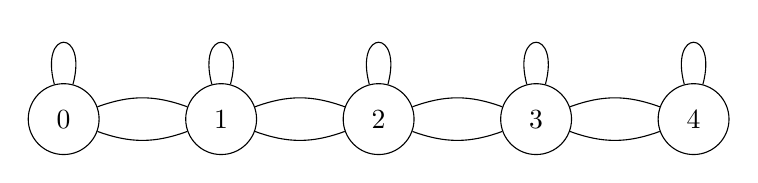
\begin{tikzpicture}[scale=1, every node/.style={circle, draw, minimum size=9mm}]
                    % Nodes
                    \node (n0) at (0,0) {0};
                    \node (n1) at (2,0) {1};
                    \node (n2) at (4,0) {2};
                    \node (n3) at (6,0) {3};
                    \node (n4) at (8,0) {4};

                    % Self-loops (simple arcs above each node)
                    \draw (n0) to[loop above] (n0);
                    \draw (n1) to[loop above] (n1);
                    \draw (n2) to[loop above] (n2);
                    \draw (n3) to[loop above] (n3);
                    \draw (n4) to[loop above] (n4);

                    % Bilateral edges between neighbors (two simple lines: one up, one down)
                    % 0 <-> 1
                    \draw (n0) to[bend left=20] (n1);
                    \draw (n1) to[bend left=20] (n0);
                    % 1 <-> 2
                    \draw (n1) to[bend left=20] (n2);
                    \draw (n2) to[bend left=20] (n1);
                    % 2 <-> 3
                    \draw (n2) to[bend left=20] (n3);
                    \draw (n3) to[bend left=20] (n2);
                    % 3 <-> 4
                    \draw (n3) to[bend left=20] (n4);
                    \draw (n4) to[bend left=20] (n3);
                \end{tikzpicture}
            \end{center}
            We never see a drawing, but \code{dsp} stores exactly this connectivity. Then:
            \begin{itemize}
                \item \code{sparisty\_pattern.copy\_from(dsp)} freezes it in a compressed format;
                \item And \code{system\_matrix.reinit(sparisty\_pattern)} allocates numeric storage \emph{only} for those $(i, j)$.
            \end{itemize}
        \end{examplebox}
        \newpage
        \item \textbf{Freeze the graph into a compressed pattern (CSR-like)}:
        \begin{lstlisting}[language=C++]
sparsity_pattern.copy_from(dsp);\end{lstlisting}
        Converts that flexible graph into a compact, cache-friendly layout (row-compressed). This step is all about \textbf{memory efficiency and fast access} downstream.

        \item \textbf{Create global Stiffness Matrix $A$}:
        \begin{lstlisting}[language=C++]
system_matrix.reinit(sparsity_pattern);\end{lstlisting}
        Where \code{sparsity\_pattern} tells which entries $(i,j)$ are allowed to exist. After this, the matrix has the right shape and memory allocated, but its entries are all zero.
        
        \item \textbf{Right-hand side}:
        \begin{lstlisting}[language=C++]
system_rhs.reinit(dof_handler.n_dofs());\end{lstlisting}
        Initializes the \textbf{right-hand side vector} $f$. Its size equals the number of global unknowns (DoFs). This vector will later be filled with the load term integrals $\displaystyle\int f \varphi_{i}$. In other words, it is the input forcing vector for the linear system.

        \item \textbf{Create Solution vector}:
        \begin{lstlisting}[language=C++]
solution.reinit(dof_handler.n_dofs());\end{lstlisting}
        Initializes the \textbf{solution vector} $u$. Same size as \code{system\_rhs}. At the beginning, it is just a vector of zeros. After solving, it will contain the approximate solution at each DoF. In other words, it is the unknown vector that will store the result after the solver runs.
    \end{itemize}
\end{enumerate}
After setup, we are ready to assemble the system: $Au = f$.
\begin{itemize}
    \item \code{system\_matrix}: $A$
    \item \code{solution}: $u$
    \item \code{system\_rhs}: $f$
\end{itemize}

\begin{center}
    \href{https://gist.github.com/AndreVale69/f04f312da68d16c253f46493ae7eaf24#file-poisson1d-cpp}{\faIcon{download} Source}
    \hspace{1em}
    \qrcode{https://gist.github.com/AndreVale69/f04f312da68d16c253f46493ae7eaf24#file-poisson1d-cpp}
\end{center}

\noindent
Output:
\begin{lstlisting}
===============================================
Setup started
Initializing the mesh
  Number of elements = 40
  Mesh saved to mesh-40.vtk
-----------------------------------------------
Initializing the finite element space
  Degree                     = 1
  DoFs per cell              = 2
  Quadrature points per cell = 2
-----------------------------------------------
Initializing the DoF handler
  Number of DoFs = 41
-----------------------------------------------
Initializing the linear system
  Initializing the sparsity pattern
  Initializing the system matrix
  Initializing the system right-hand side
  Initializing the solution vector\end{lstlisting}
    \paragraph[Assemble: compute \texorpdfstring{$A$}{A} and \texorpdfstring{$f$}{f}]{Assemble: compute $A$ and $f$}

This is the part at the top of \code{assemble()}:
\begin{lstlisting}[language=C++]
// Number of local DoFs for each element.
const unsigned int dofs_per_cell = fe->dofs_per_cell;

// Number of quadrature points for each element.
const unsigned int n_q = quadrature->size();

// FEValues instance.
// This object allows to compute basis functions, their
// derivatives, the reference-to-current element mapping
// and its derivatives on all quadrature points
// of all elements.
FEValues<dim> fe_values(
    *fe,
    *quadrature,
    // Here we specify what quantities we need FEValues
    // to compute on quadrature points.
    // For our test, we need:
    // - the values of shape functions
    // - the derivative of shape functions
    // - the position of quadrature points
    // - the product J_c(x_q)*w_q
    update_values |
    update_gradients |
    update_quadrature_points |
    update_JxW_values
);

// Local matrix and right-hand side vector.
// We will overwrite them for each element within the loop.
FullMatrix<double> cell_matrix(dofs_per_cell, dofs_per_cell);
Vector<double>     cell_rhs(dofs_per_cell);

// We will use this vector to store the global indices
// of the DoFs of the current element within the loop.
std::vector<types::global_dof_index> dof_indices(dofs_per_cell);

// Reset the global matrix and vector, just in case.
system_matrix = 0.0;
system_rhs    = 0.0;\end{lstlisting}
\begin{itemize}
    \item \important{\code{dofs\_per\_cell}}. Each element (cell) of the mesh has its own set of \emph{local} basis functions (shape functions). This number depends on:
    \begin{itemize}
        \item The finite element type (\code{FE\_Q<dim>(r)} $\rightarrow$ polynomial degree);
        \item The dimension (\code{dim}).
    \end{itemize}
    For example, 1D linear elements ($r=1$), then 2 local DoFs per cell.


    \item \important{\code{n\_q = quadrature->size()}}. Quadrature rule defines how many integration points we use \emph{per cell}. Needed because we approximate integrals by weighted sums at quadrature points.


    \item \important{\code{FEValues} object}. This is the \textbf{bridge between reference element and physical cell}. It knows how to evaluate:
    \begin{itemize}
        \item Values of shape functions (\code{update\_values})
        \item Gradients of shape functions (\code{update\_gradients})
        \item Coordinates of quadrature points (\code{update\_quadrature\_points})
        \item Jacobian $\times$ weight factors (\code{update\_JxW\_values})
    \end{itemize}
    Essentially, this object does all the geometric bookkeeping for us.

    \textcolor{Green3}{\faIcon{question-circle} \textbf{Why is \code{FEValues} needed?}}
    \begin{itemize}
        \item[\textcolor{Green3}{\faIcon{question-circle}}] \textcolor{Green3}{\textbf{What we want to compute.}} From laboratory 1, we know the weak form turns into local contributions like (page \pageref{eq: stiffness matrix}):
        \begin{equation*}
            A^{(K)}_{ij} = \int_{K} \mu(x) \cdot \nabla \varphi_i(x) \cdot \nabla \varphi_j(x) \, \mathrm{d}x
        \end{equation*}
        And (page \pageref{eq: nodal forces}):
        \begin{equation*}
            f^{(K)}_{i} = \int_{K} f(x) \cdot \varphi_i(x)\, \mathrm{d}x
        \end{equation*}
        For each element $K$. So we need:
        \begin{itemize}
            \item Basis functions $\varphi_i(x)$;
            \item Their gradients $\nabla \varphi_i(x)$;
            \item Quadrature weights and Jacobians for mapping integrals from reference element to physical cell.
        \end{itemize}

        
        \item[\textcolor{Red2}{\faIcon{times-circle}}] \textcolor{Red2}{\textbf{The ``manual'' alternative.}} In principle we could:
        \begin{enumerate}
            \item Hard-code the formulas for each basis function;
            \item Transform coordinates from the reference element (e.g. $[-1,1]$) to the physical element;
            \item Compute the Jacobian determinant $J$ and its inverse transpose for gradients;
            \item Loop over quadrature nodes, evaluating shape functions and gradients by hand.
        \end{enumerate}
        This is \textbf{tedious, error-prone, and messy} (especially in 2D/3D or for higher order elements).


        \item[\textcolor{Green3}{\faIcon{check-circle}}] \textcolor{Green3}{\textbf{What \code{FEValues} does.}} \code{FEValues} is the \textbf{automation tool}:
        \begin{itemize}
            \item Given:
            \begin{itemize}
                \item The finite element space (\code{FE\_Q}),
                \item The quadrature rule (\code{QGauss}),
                \item The flags (\code{update\_values | update\_gradients | ...}),
            \end{itemize}
            \item It precomputes, for \textbf{all quadrature points of a given cell}:
            \begin{itemize}
                \item $\varphi_i(x_q)$ $\rightarrow$ basis values;
                \item $\nabla \varphi_i(x_q)$ $\rightarrow$ basis gradients, mapped to physical cell;
                \item $x_q$ $\rightarrow$ actual coordinates of quadrature points;
                \item $J(x_q) w_q$ $\rightarrow$ the correct measure for integration.
            \end{itemize}
        \end{itemize}
        So instead of writing integrals by hand, we just write:
        \begin{lstlisting}[language=C++]
fe_values.shape_value(i, q)
fe_values.shape_grad(i, q)
fe_values.quadrature_point(q)
fe_values.JxW(q)\end{lstlisting}
        And it gives the correct quantity.
    \end{itemize}


    \item \important{Local containers (\code{cell\_matrix}, \code{cell\_rhs})}. Each cell contributes a \textbf{local stiffness matrix} and a \textbf{local load vector}. These are small (size $=$ \code{dofs\_per\_cell} $\times$ \code{dofs\_per\_cell}). We recompute them for each element, then add them into the big global system.
    

    \item \important{\code{dof\_indices} vector}. Temporary storage: maps local DoFs of the cell to global DoF indices. For example, on cell 3, local DoFs might correspond to global DoFs \code{[5, 6]}.
    

    \item \important{Reset global system}. Before assembly, set matrix and RHS to zero, so we don't accumulate leftovers from a previous call.
\end{itemize}

\begin{flushleft}
    \textcolor{Green3}{\faIcon{tools} \textbf{Element-wise assembly of local matrices and vectors into the global system}}
\end{flushleft}
\begin{lstlisting}[language=C++]
for (const auto &cell : dof_handler.active_cell_iterators())
{
    // Reinitialize the FEValues object on current element.
    // This precomputes all the quantities we requested when
    // constructing FEValues (see the update_* flags above)
    // for all quadrature nodes of the current cell.
    fe_values.reinit(cell);

    // We reset the cell matrix and vector
    // (discarding any leftovers from previous element).
    cell_matrix = 0.0;
    cell_rhs    = 0.0;

    for (unsigned int q = 0; q < n_q; ++q)
    {
        // Here we assemble the local contribution for
        // current cell and current quadrature point,
        // filling the local matrix and vector.

        // Here we iterate over *local* DoF indices.
        for (unsigned int i = 0; i < dofs_per_cell; ++i)
        {
            for (unsigned int j = 0; j < dofs_per_cell; ++j)
            {
                // FEValues::shape_grad(i, q) returns
                // the gradient of the i-th basis function
                // at the q-th quadrature node, already mapped
                // on the physical element:
                // we don't have to deal with the
                // mapping, it's all hidden inside FEValues.
                cell_matrix(i, j) += diffusion_coefficient.value(
                    fe_values.quadrature_point(q))  // mu(x)
                    * fe_values.shape_grad(i, q)    // (I)
                    * fe_values.shape_grad(j, q)    // (II)
                    * fe_values.JxW(q);             // (III)
            }

            cell_rhs(i) += forcing_term.value(
                fe_values.quadrature_point(q)
            ) * fe_values.shape_value(i, q) * fe_values.JxW(q);
        }
    }

    // At this point the local matrix and
    // vector are constructed: we need to sum them into the
    // global matrix and vector. To this end, we need to
    // retrieve the global indices of the DoFs of current cell.
    cell->get_dof_indices(dof_indices);

    // Then, we add the local matrix and vector into
    // the corresponding positions of the global matrix
    // and vector.
    system_matrix.add(dof_indices, cell_matrix);
    system_rhs.add(dof_indices, cell_rhs);
}\end{lstlisting}
\begin{itemize}
    \item \important{\code{for (const auto \&cell : dof\_handler.active\_cell\_iterators())}} \code{dof\_handler} is the object that knows the mesh (triangulation) and the distribution of DoFs on it. \code{active\_cell\_iterators()} returns \textbf{iterators to all active cells} in the mesh.
    
    \textcolor{Green3}{\faIcon{question-circle} \textbf{What is an \emph{active cell}?}} \code{deal.II} supports \textbf{adaptive meshes}: some cells can be refined into smaller children. The \textbf{active cells} are those that are \textbf{leaves of the refinement tree}, i.e. the cells we actually want to assemble on. If we're using a uniform mesh (like in our laboratory), then \textbf{all cells are active}. So this loop literally means: ``\emph{for each element of the mesh on which the solution is represented, do the following steps}''.

    \textcolor{Green3}{\faIcon{question-circle} \textbf{Why loop over cells?}} Finite element assembly is \textbf{element-by-element}:
    \begin{enumerate}
        \item Compute the \emph{local} contributions (cell matrix and RHS).
        \item Scatter them into the \emph{global} system.
    \end{enumerate}
    That's why we need to visit each cell in turn.


    \item \important{\code{fe\_values.reinit(cell);}} \code{fe\_values} was created outside the loop with a finite element (\code{fe}), a quadrature rule (\code{quadrature}), and some update flags (\code{update\_values}, \code{update\_gradients}, ...). However, at that particular moment, it was not linked to any specific cell. So, calling \code{reinit(cell)} means: ``\emph{take this cell, map the reference element to its physical shape, and precompute all the quantities we asked for at quadrature points (shape values, gradients, JxW, coordinates, ...)}''.

    \textcolor{Green3}{\faIcon{question-circle} \textbf{Why it's necessary.}} Every cell can have different geometry (different size, position, refinement). The mapping (and therefore Jacobian, gradients, quadrature point positions) changes per cell. \code{reinit(cell)} makes sure that \code{fe\_values.shape\_grad(i,q)} or \code{fe\_values.JxW(q)} (see below) correspond to \textbf{this specific cell}.


    \item \important{\code{cell\_matrix = 0.0; cell\_rhs = 0.0;}} These two variables are the \textbf{local contributions} for the current cell. They are small (size $=$ \code{dofs\_per\_\break cell} $\times$ \code{dofs\_per\_cell} for the matrix, and \code{dofs\_per\_cell} for the RHS). Since we are looping over all cells, we need to \textbf{clear them out} before computing the contributions for this cell. Otherwise, leftovers from the previous cell would pollute the new computations.
    

    \item \important{\code{for (unsigned int q = 0; q < n\_q; ++q) \{...\}}}. \textbf{Iterate all quadrature points on the current cell} to accumulate the cell's local matrix and RHS via numerical integration.
    
    \textcolor{Green3}{\faIcon{question-circle} \textbf{Why it exists.}} Our integrals:
    \begin{equation*}
        A^{(K)}_{ij} = \int_K \mu\cdot \nabla\phi_{i} \cdot \nabla\phi_j\,\mathrm{d}x, \qquad f^{(K)}_{i} = \int_K f\cdot \phi_i\,\mathrm{d}x
    \end{equation*}
    Are \textbf{approximated by sums} over quadratures nodes $x_{q}$:
    \begin{equation*}
        \begin{array}{rcl}
            A^{(K)}_{ij} &\approx& \displaystyle\sum_{q=1}^{n_q}\mu(x_q)\cdot \nabla\phi_i(x_q) \cdot \nabla\phi_j(x_q) \cdot JxW(q) \\[.5em]
            f^{(K)}_{i} &\approx& \displaystyle\sum_{q=1}^{n_q} f(x_q) \cdot \phi_{i}(x_{q}) \cdot JxW(q)
        \end{array}
    \end{equation*}
    Here $JxW(q)$ is the mapped weight $\left|\det J_{K}\right| \cdot w_{q}$ from the reference element to the physical cell.

    \textcolor{Green3}{\faIcon{question-circle} \textbf{What are $x_q$?}} They are the \textbf{quadrature points}, i.e. the positions inside each cell where the integral is sampled. When we replace integrals with quadrature, we need both:
    \begin{itemize}
        \item the \textbf{weights} $w_q$ (how much each sample contributes);
        \item the \textbf{points} $x_q$ (where to evaluate the integrand).
    \end{itemize}
    So $x_q$ are the specific coordinates where we evaluate the shape functions, their gradients, and the data $f(x)$, $\mu(x)$, etc.

    \textcolor{Green3}{\faIcon{question-circle} \textbf{Why do we need them?}} Look at our weak form:
    \begin{equation*}
        a(u,v) = \int_{\Omega} \mu(x) \cdot \nabla u(x) \cdot \nabla v(x)\,\mathrm{d}x, \qquad F(v) = \int_{\Omega} f(x) \cdot v(x)\,\mathrm{d}x
    \end{equation*}
    The quadrature approximation is:
    \begin{equation*}
        a(u,v) \;\approx\; \sum_{q=1}^{n_q} \mu(x_q) \cdot \nabla u(x_q) \cdot \nabla v(x_q) \cdot JxW(q)
    \end{equation*}
    \begin{equation*}
        F(v) \;\approx\; \sum_{q=1}^{n_q} f(x_q) \cdot v(x_q) \cdot JxW(q)
    \end{equation*}
    Here we see explicitly: we need to know \textbf{where} to evaluate $\mu(x)$, $f(x)$, $\phi_{i}(x)$, $\nabla\phi_i(x)$. That ``where'' is exactly the quadrature point $x_q$.

    \textcolor{Green3}{\faIcon{question-circle} \textbf{Where does $JxW(q)$ come from?}} In FEM, we don't integrate directly on each physical cell $K$. We map everything back to a \textbf{reference cell} $\hat{K}$ (like $[-1,1]$ in 1D, the unit square in 2D, ...). The map $F_K : \hat{K} \to K$ has a \textbf{Jacobian matrix}:
    \begin{equation}
        J_{K}\left(\hat{\xi}\right) = \dfrac{\partial x}{\partial \hat{\xi}}
    \end{equation}
    When we change variables in an integral, the measure transforms as:
    \begin{equation*}
        \int_{K} g(x)\, \mathrm{d}x = \int_{\hat{K}} g\left(F_{K}\left(\hat{\xi}\right)\right) \cdot \left|\det J_{K}\left(\hat{\xi}\right)\right| \, \mathrm{d}\hat{\xi}
    \end{equation*}
    On the reference cell, we approximate the integral with quadrature:
    \begin{equation*}
        \int_{\hat{K}} g\left(F_{K}\left(\hat{\xi}\right)\right) \cdot \left|\det J_{K}\left(\hat{\xi}\right)\right| \, \mathrm{d}\hat{\xi}
        \;\approx\;
        \displaystyle\sum_{q=1}^{n_q} g\left(F_K\left(\hat{\xi}_q\right)\right) \cdot \left|\det J_K\left(\hat{\xi}_q\right)\right| \cdot w_{q}
    \end{equation*}
    Where $w_q$ are the quadrature weights on $\hat{K}$.

    \code{deal.II} packages the product:
    \begin{equation*}
        \left|\det J_K\left(\hat{\xi}_q\right)\right| \cdot w_q
    \end{equation*}
    Into one quantity:
    \begin{lstlisting}
fe_values.JxW(q)\end{lstlisting}

    \textcolor{Green3}{\faIcon{question-circle} \textbf{Why we need it.}} If we didn't multiply by $JxW(q)$:
    \begin{itemize}
        \item Our integral would be computed as if the cell had \textbf{unit size and shape}.
        \item For example, in 1D, integrating over $\left[0,h\right]$ would give the same result as over $\left[0,1\right]$.
        \item That's completely wrong: the measure (length, area, volume) of each cell must appear in the integral.
    \end{itemize}
    $JxW(q)$ is the \textbf{correct measure of the little piece of the cell around quadrature point} $x_{q}$.


    \item \important{\code{for (unsigned int i = 0; i < dofs\_per\_cell; ++i) \{...\}}}. Each\break cell has \code{dofs\_per\_cell} local shape functions $\left\{\varphi_{i}\right\}$. This loop means: ``\emph{for each local basis function $\varphi_{i}$ on this element, compute its contribution}''.
    
    \textcolor{Green3}{\faIcon{question-circle} \textbf{Why is it needed?}}
    \begin{enumerate}
        \item \textbf{For the matrix} $A^{(K)}$ we need contributions for every pair $\left(i,j\right)$. That's why inside this loop there's another nested loop over \code{j}. So we fill an entries of the local stiffness matrix.
        \item \textbf{For the RHS} $f^{(K)}$ each equation corresponds to a test function $\varphi_{i}$. So for each \code{i}, we compute:
        \begin{equation*}
            f^{(K)}_{i} \approx \displaystyle\sum_q f\left(x_{q}\right) \cdot \varphi_{i}\left(x_{q}\right) \cdot JxW(q)
        \end{equation*}
    \end{enumerate}


    \item \important{Fill Stiffness Matrix}
    \begin{lstlisting}[language=C++]
for (unsigned int j = 0; j < dofs_per_cell; ++j) {
    cell_matrix(i, j) += diffusion_coefficient.value(
        fe_values.quadrature_point(q))  // mu(x)
        * fe_values.shape_grad(i, q)    // (I)
        * fe_values.shape_grad(j, q)    // (II)
        * fe_values.JxW(q);             // (III)
}\end{lstlisting}
    Inside the surrounding loops over the cell and the quadrature point $q$, that line accumulates the quadrature contribution to:
    \begin{equation*}
        A^{(K)}_{ij} \;\approx\; \displaystyle\sum_{q=1}^{n_{q}} \mu(x_q) \cdot \nabla\phi_{i}\left(x_{q}\right) \cdot \nabla\phi_{j}\left(x_{q}\right) \cdot JxW(q)
    \end{equation*}
    Which is the discrete version of:
    \begin{equation*}
        A^{(K)}_{ij} = \displaystyle\int_{K} \mu(x) \cdot \nabla\phi_i(x) \cdot \nabla\phi_j(x)\,\mathrm{d}x \; \text{(local form)}
    \end{equation*}
    Summing over all cells later gives the global entries $A_{ij}$ used in $A\, u = f$.

    A few precise points about what happens here:
    \begin{itemize}
        \item \textbf{Role of} $j$: for a fixed $i$, we pair the test function $\phi_i$ with every trial function $\phi_j$ on the cell. That's why this loop runs over all local DoFs. The result is the full dense local matrix $\left(A^{(K)}_{ij}\right)_{i,j=0}^{\text{dofs\_per\_cell}-1}$.
        
        \item \textbf{What each factor supplies}:
        \begin{itemize}
            \item $\mu(x_q)$ is:
            \begin{lstlisting}[language=C++]
diffusion_coefficient.value(
    fe_values.quadrature_point(q)
)\end{lstlisting}
            \item \code{fe\_values.shape\_grad(i,q)} is $\nabla\phi_i(x_q)$ in \textbf{physical} coordinates.
            \item \code{fe\_values.shape\_grad(j,q)} is $\nabla\phi_j(x_q)$.
            \item \code{fe\_values.JxW(q)} is the mapped weight $\left|\det J_K\left(\hat{\xi}_q\right)\right| \cdot w_q$.
        \end{itemize}

        \item \textbf{Symmetry}: since $\nabla\phi_i\cdot\nabla\phi_j = \nabla\phi_j\cdot\nabla\phi_i$ and $\mu\ge 0$, the local (and global) matrix is symmetric: $A_{ij}=A_{ji}$. Many codes exploit this to halve work, but it's fine (and clearer) to assemble all $(i,j)$.

        \item \textbf{Cost structure}: the nested \code{i,j} loops make the local work $O(n_q \cdot \code{dofs\_per\_cell}^2)$ per cell (big $O$ notation). For $r=1$ in 1D, $\code{dofs\_}\break\code{per\_cell}=2$, so this is tiny; in higher order/dimension, careful placement of the \code{mu(x\_q)} load (hoist it outside the \code{j} loop), and reuse of \code{shape\_grad(i,q)} values help with performance.
        
        \item \textbf{Connection to the notes}: the exact same bilinear form shown in our laboratory 1 solution:
        \begin{equation*}
            A_{ij} = a\left(\phi_j,\phi_i\right)=\displaystyle\int_{\Omega} \mu \cdot \phi_{j}' \cdot \phi_{i}'\,\mathrm{d}x
        \end{equation*}
        Is what we're discretizing here via quadrature on each cell.
    \end{itemize}
    After this \code{j} loop finishes (for the current $i$ and current $q$), we've added the $q$-th quadrature contribution to the entire \textbf{row} $i$ of the local matrix. The outer loops over $q$ (quadrature points) and then over $i$ complete the whole local matrix for the cell; afterwards we scatter it to the global matrix with \code{system\_matrix.add(dof\_indices, cell\_matrix)}.


    \item \important{Assemble load vector (right-hand side)}
    \begin{lstlisting}[language=C++]
cell_rhs(i) += forcing_term.value(
                fe_values.quadrature_point(q)
               ) * fe_values.shape_value(i, q) *
               fe_values.JxW(q);\end{lstlisting}
    We start from the weak formulation of the Poisson problem:
    \begin{equation*}
        a(u, v) = F(v), \quad \forall v \in V
    \end{equation*}
    With:
    \begin{equation*}
        a(u,v) = \int_{\Omega} \mu(x) \cdot u'(x) \cdot v'(x)\, \mathrm{d}x, 
        \quad
        F(v) = \int_{\Omega} f(x) \cdot v(x)\, \mathrm{d}x 
    \end{equation*}
    When we discretize, the \textbf{load vector entry} for basis/test function $\phi_{i}$ is:
    \begin{equation*}
        f_{i} = \int_{\Omega} f(x) \cdot \phi_i(x)\, \mathrm{d}x
    \end{equation*}
    In the code each part corresponds to the quadrature approximation of this integral:
    \begin{itemize}
        \item \important{\code{forcing\_term.value(fe\_values.quadrature\_point(q))}} is $f(x_{q})$, the source term evaluated at the quadrature point $x_{q}$.
        
        \item \important{\code{fe\_values.shape\_value(i, q)}} is $\phi_{i}(x_{q})$, the value of the $i$-th basis (test) function at the quadrature point.
        
        \item \important{\code{fe\_values.JxW(q)}} is the \textbf{Jacobian times weight}, it converts the integral over a possibly deformed cell into a sum of weighted contributions at quadrature points. Formally, it's:
        \begin{equation*}
            JxW(q) = \det\left(J_T\left(x_q\right)\right) \cdot w_q
        \end{equation*}
        Where $\det(J_{T})$ is the Jacobian determinant of the mapping from the reference element, and $w_{q}$ is the quadrature weight.

        \item \important{\code{cell\_rhs(i) += ...}} we sum these contributions over all quadrature points $q$. This approximates:
        \begin{equation*}
            f_i \approx \sum_q f(x_q) \cdot \phi_i(x_q) \cdot JxW(q)
        \end{equation*}
    \end{itemize}
    This line is building the discrete version of the \textbf{load vector}. For each degree of freedom (basis function $\phi_{i}$), it accumulates the weighted contributions of the source term $f$ over the cell, using numerical quadrature. We can think of it as: ``\emph{take the forcing term at each integration point, multiply by the shape function, scale by the correct measure of volume (\code{JxW}), and sum them up to get the correct right-hand-side entry}''.


    \item \important{\code{cell->get\_dof\_indices(dof\_indices);}}
    
    \textcolor{Green3}{\faIcon{book} \textbf{The context.}} Up to this point, we've assembled the \textbf{local stiffness matrix} (\code{cell\_matrix}) and the \textbf{local load vector} (\code{cell\_rhs}) for one element (\code{cell}). These are written in terms of the \textbf{local basis functions} on that cell. But the \textbf{global linear system} is assembled in terms of \textbf{global degrees of freedom (DoFs)}, one big vector \code{u} and one big matrix \code{A} for the whole mesh. So, we need a map: \emph{which global indices do our local basis functions correspond to?}

    \textcolor{Green3}{\faIcon{question-circle} \textbf{What does \code{get\_dof\_indices} do?}} Each \code{cell} in \code{deal.II} has a small number of \textbf{local DoFs} (e.g. 2 in 1D linear case, 3 in quadratic case, etc.). The method:
    \begin{lstlisting}
cell->get_dof_indices(dof_indices);\end{lstlisting}
    Fills the vector \code{dof\_indices} with the \textbf{global numbering} assigned to those local DoFs by the \code{DoFHandler}. For example, in 1D with $N=3$ cells, linear elements (\code{r=1}):
    \begin{itemize}
        \item Nodes: $x_0, x_1, x_2, x_3$.
        \item Global DoFs: numbered \code{[0,1,2,3]}.
        \item Cell 0 (interval $[x_0, x_1]$): local DoFs $\to$ global indices \code{[0,1]}.
        \item Cell 1 ($[x_1, x_2]$): local DoFs $\to$ \code{[1,2]}.
        \item Cell 2 ($[x_2, x_3]$): local DoFs $\to$ \code{[2,3]}.
    \end{itemize}
    When we call \code{get\_dof\_indices} on cell 1, we'll get \code{{1,2}}.

    \begin{examplebox}[: Physical analogy]
        Think of each \textbf{cell} like a small team in a company:
        \begin{itemize}
            \item Locally, the team has roles ``\code{Alice = i=0}, \code{Bob = i=1}''.
            \item But globally, \code{Alice} is employee \code{\#123}, \code{Bob} is employee \code{\#124} in the company's HR system.
            \item \code{get\_dof\_indices} is the lookup that tells us ``local slot $\to$ global employee number'', so we can update the \textbf{global payroll system} (the linear system) correctly.
        \end{itemize}
    \end{examplebox}


    \item \important{Scatter-Add from the element (\code{cell}) to the global system}
    \begin{lstlisting}[language=C++]
system_matrix.add(dof_indices, cell_matrix);
system_rhs.add(dof_indices, cell_rhs);\end{lstlisting}
    They are just compact shorthands for the ``triple loop'' we'd otherwise write:
    \begin{itemize}
        \item \textbf{Matrix}
        \begin{lstlisting}[language=C++]
for (unsigned int i = 0; i < dofs_per_cell; ++i)
    for (unsigned int j = 0; j < dofs_per_cell; ++j)
        system_matrix.add(
            dof_indices[i],
            dof_indices[j],
            cell_matrix(i,j)
        );\end{lstlisting}
        This adds each local entry $\left(A^{K}\right)_{ij}$ into the \textbf{global} entry $A_{\text{glob}(i),\text{glob}(j)}$
        \item \textbf{RHS vector}
        \begin{lstlisting}[language=C++]
for (unsigned int i = 0; i < dofs_per_cell; ++i)
    system_rhs(dof_indices[i]) += cell_rhs(i);\end{lstlisting}
        This adds the local load entry $f^{K}_{i}$ into the global $f_{\text{glob}(i)}$.
    \end{itemize}
    Here \code{dof\_indices[i]} is exactly the global DoF index for the $i$-th local basis function (provided by \code{cell->get\_dof\_indices(...)}), so each cell contributes to the \textbf{same} global rows/columns where nodes are shared. Over all cells, these adds build the global linear system $Au=f$ (the discrete version of $a(u,v)=F(v)$).
\end{itemize}

\begin{flushleft}
    \textcolor{Red2}{\faIcon{exclamation-triangle} \textbf{Boundary Conditions}}
\end{flushleft}
\begin{lstlisting}[language=C++]
// Boundary conditions.
{
    // We construct a map that stores,
    // for each DoF corresponding to a Dirichlet condition,
    // the corresponding value.
    // E.g., if the Dirichlet condition is
    // u_i = b, the map will contain the pair (i, b).
    std::map<types::global_dof_index, double> boundary_values;

    // This object represents our boundary data
    // as a real-valued function
    // (that always evaluates to zero).
    Functions::ZeroFunction<dim> bc_function;

    // Then, we build a map that,
    // for each boundary tag, stores the
    // corresponding boundary function.
    std::map<
        types::boundary_id,
        const Function<dim> *
    > boundary_functions;
    boundary_functions[0] = &bc_function;
    boundary_functions[1] = &bc_function;

    // interpolate_boundary_values fills
    // the boundary_values map.
    VectorTools::interpolate_boundary_values(
        dof_handler,
        boundary_functions,
        boundary_values
    );

    // Finally, we modify the linear system
    // to apply the boundary conditions.
    // This replaces the equations
    // for the boundary DoFs with the corresponding
    // u_i = 0 equations.
    MatrixTools::apply_boundary_values(
        boundary_values,
        system_matrix,
        solution,
        system_rhs,
        true
    );
}\end{lstlisting}
\begin{itemize}
    \item \important{\code{std::map<types::global\_dof\_index,double> boundary\_values}} is essentially preparing a \textbf{container to store Dirichlet boundary conditions}.
    \begin{itemize}
        \item \code{types::global\_dof\_index} is just \code{deal.II}'s typedef for an unsigned integer that labels a degree of freedom (DoF) in the \textbf{global numbering} created by the \code{DoFHandler}. Every unknown of the system (i.e. each node where we want to compute the solution) gets such an index.
        \item \code{double} is the prescribed value of the solution at that DoF, coming from the boundary condition.
    \end{itemize}
    So this \code{map} will be filled later with pairs of the form:
    \begin{equation*}
        (i, b) \quad \text{meaning: DoF } i \text{ must take the value } b.
    \end{equation*}
    For our Poisson 1D (with homogeneous Dirichlet BCs $u(0)=u(1)=0$), this means we will eventually store something like:
    \begin{itemize}
        \item \code{(DoF index at x=0, 0.0)}
        \item \code{(DoF index at x=1, 0.0)}
    \end{itemize}
    And possibly more if the mesh has multiple boundary faces. In other words, this line declares a data structure that will \textbf{hold all the boundary constraints} needed to later enforce them in the linear system. 


    \item \important{\code{Functions::ZeroFunction<dim> bc\_function;}} creates an object that represents the \textbf{mathematical function $u(x)=0$} in the whole domain of dimension \code{dim}.
    \begin{itemize}
        \item \code{Functions::ZeroFunction<dim>} is a class provided by \code{deal.II} that inherits from \code{Function<dim>}.
        \item It is a simple function object: whenever we evaluate it at some point $x \in \mathbb{R}^\text{dim}$, it always returns \code{0.0}.
        \item The template parameter \code{<dim>} just means it works in 1D, 2D, or 3D, depending on our problem setup.
    \end{itemize}

    \textcolor{Green3}{\faIcon{question-circle} \textbf{Why do we need it?}} Because boundary conditions in \code{deal.II} are expressed as \textbf{functions defined on the boundary}. Even if the condition is simply homogeneous Dirichlet ($u=0$), we still need to pass a function object. So here, \code{bc\_function} is the \emph{prescribed boundary function} that tells the solver: ``\emph{on the boundary, the solution must equal zero}''.

    Later on, this object is associated with the boundary ids (e.g. left and right ends of the interval in 1D), and then interpolated into the discrete finite element space to actually generate the values for each boundary DoF.


    \item \important{Set the Dirichlet functions}
    \begin{lstlisting}[language=C++]
std::map<
    types::boundary_id,
    const Function<dim> *
> boundary_functions;
boundary_functions[0] = &bc_function;
boundary_functions[1] = &bc_function;\end{lstlisting}
    First of all, we prepare a \code{map} between boundary identifiers and the corresponding \emph{boundary conditions}.
    \begin{itemize}
        \item \code{types::boundary\_id} is just a \code{deal.II} typedef (an integer type) used to \textbf{tag different parts of the boundary} of the mesh.
        \item The value is a pointer to a \code{const Function<dim>} object, because different boundaries may have different prescribed functions.
    \end{itemize}
    So this \code{map} will tell \code{deal.II} ``\emph{on boundary with id X, apply function Y as boundary condition}''.

    About assignments:
    \begin{itemize}
        \item \code{boundary\_functions[0] = \&bc\_function;} Boundary with \code{id = 0} (e.g. in 1D, this corresponds to $x=0$) is assigned the function \code{bc\_function}. Recall \code{bc\_function} is \code{ZeroFunction<dim>}, so: ``\emph{on boundary 0, impose \code{u = 0}}''.
        \item \code{boundary\_functions[1] = \&bc\_function;} Boundary with \code{id = 1} (e.g. in 1D, the point $x = 1$) is also assigned the same zero function. So ``\emph{on boundary 1, impose \code{u = 0}}''.
    \end{itemize}

    \textcolor{Green3}{\faIcon{question-circle} \textbf{Why two lines?}} In our lab problem (Poisson in 1D), the domain is $\Omega = \left(0, 1\right)$ and the BCs are homogeneous Dirichlet:
    \begin{equation*}
        u(0)=0, \quad u(1)=0
    \end{equation*}
    \code{deal.II} distinguishes boundaries using IDs. By default: left endpoint of the 1D interval $\to$ \code{id 0}; right endpoint $\to$ \code{id 1}. So we explicitly say: \textbf{both boundary ids (0 and 1) are constrained with the zero Dirichlet function}.


    \item \important{Computes boundary condition values}
    \begin{lstlisting}[language=C++]
VectorTools::interpolate_boundary_values(
    dof_handler,
    boundary_functions,
    boundary_values
);\end{lstlisting}
    This function from \code{deal.II} \textbf{computes the actual values of the boundary conditions on the degrees of freedom (DoFs) that live on the boundary}, and fills the \code{boundary\_values} map we created earlier.
    \begin{enumerate}
        \item \textbf{Inputs}
        \begin{itemize}
            \item \code{dof\_handler}: knows the finite element space and which DoFs are attached to which cells/faces. It can tell us which DoFs sit on the boundary.
            \item \code{boundary\_functions}: the map that says: ``\emph{on boundary \code{id = X}, apply function \code{Y}}''.
            \item \code{boundary\_values}: the map that will be filled.
        \end{itemize}
        \item \textbf{Interpolation process}
        \begin{itemize}
            \item For each boundary id in \code{boundary\_functions}, \code{deal.II} finds all the DoFs lying on that boundary part.
            \item It then evaluates the corresponding function (here \code{bc\_function}, i.e. always \code{0.0}) at the DoF locations.
            \item It records the pair \code{(global\_dof\_index, value)} into \code{boundary\_values}.
        \end{itemize}
        \item \textbf{Result}: after this call, \code{boundary\_values} contains entries like:
        \begin{equation*}
            \left\{0 \to 0.0, 19 \to 0.0\right\}
        \end{equation*}
        Assuming DoF and DoF 19 happen to be the endpoints of our 1D mesh with 20 subintervals.
    \end{enumerate}

    \textcolor{Green3}{\faIcon{question-circle} \textbf{Why is this interpolation needed?}} Because the function is continuous (mathematical), but the finite element solution space is discrete: it only knows about DoFs. We must translate ``\emph{$u(x)=0$ on boundary}'' into ``\code{DoF \#i = 0.0}'' for every DoF lying on the boundary. So this line is the \textbf{bridge} between the abstract boundary condition (function on the boundary) and the concrete algebraic system (specific entries in vectors/matrices).


    \item \important{Impose Dirichlet BCs on the linear system}
    \begin{lstlisting}[language=C++]
MatrixTools::apply_boundary_values(
    boundary_values,
    system_matrix,
    solution,
    system_rhs,
    true
);\end{lstlisting}
    Inputs:
    \begin{itemize}
        \item \code{boundary\_values}: the map $\{ i \mapsto b_i \}$ saying ``\emph{DoF $i$ must take value $b_i$}''.
        \item \code{system\_matrix} $A$, \code{system\_rhs} $f$, and the current \code{solution} vector $u$ (used/updated).
        \item The last flag \code{true} means \textbf{also eliminate columns} (keeps the system symmetric and clean).
    \end{itemize}

    \textcolor{Green3}{\faIcon{stream} \textbf{What \code{apply\_boundary\_values} does (Dirichlet enforcement).}} For each constrained DoF $i$ in \code{boundary\_values}:
    \begin{enumerate}
        \item \textbf{Zero the entire row $i$} of $A$.
        \item \textbf{Put a 1 on the diagonal}: $A_{ii} \leftarrow 1$.
        \item \textbf{Set the RHS}: $f_{i} \leftarrow b_{i}$.
        \item If \code{eliminate\_columns == true} (our case), \textbf{also zero column $i$} and \textbf{correct the RHS} of the \emph{unconstrained} equations to account for the known value $u_{i} = b_{i}$:
        \begin{equation*}
            f_j \leftarrow f_j - A_{j i}^{\text{(old)}} \cdot b_i \quad \text{for all unconstrained } j
        \end{equation*}
        Then set $A_{j i} \leftarrow 0$ for all $j \neq i$.
        \item \textbf{Set the solution entry}: $u_{i} \leftarrow b_{i}$ (so the vector is consistent for output/initial guesses).
    \end{enumerate}
    Net effect: the $i$-th equation becomes exactly $u_{i} = b_{i}$ and the rest of the system is modified so those fixed values no longer appear implicitly on the left-hand side.
    
    \textcolor{Green3}{\faIcon{question-circle} \textbf{Why the last \code{true} matters}}
    \begin{itemize}
        \item \code{true} (\textbf{eliminate columns}): preserves symmetry/positive definiteness (important for CG), avoids spurious nonzeros, and makes the algebra cleaner.
        \item \code{false}: leaves columns intact; sometimes used to keep certain preconditioner patterns, but less common for symmetric SPD problems.
    \end{itemize}
    So this single call rewrites our system so that \textbf{boundary DoFs are hard-set to the prescribed values} and the remaining unknowns solve a system that already accounts for those fixed notes.
\end{itemize}
In conclusion, the assembly routine builds the algebraic system corresponding to our PDE. First, it computes the local stiffness matrices and load vectors on each element using quadrature, then it inserts them into the global matrix and right-hand side. Finally, boundary conditions are enforced by directly modifying the system so that boundary DoFs take the prescribed values. After this step, the discrete problem is fully defined as a linear system $Au = f$, ready to be solved with the chosen linear solver.

\begin{center}
    \href{https://gist.github.com/AndreVale69/f04f312da68d16c253f46493ae7eaf24#file-poisson1d-cpp}{\faIcon{download} Source}
    \hspace{1em}
    \qrcode{https://gist.github.com/AndreVale69/f04f312da68d16c253f46493ae7eaf24#file-poisson1d-cpp}
\end{center}


    %%%%%%%%%%%%%%%%%%%%%%%%%%
    % Bibliography and index %
    %%%%%%%%%%%%%%%%%%%%%%%%%%
    \pagestyle{fancy}
\fancyhead{} % clear all header fields
\fancyhead[R]{\nouppercase{\leftmark\hfill\rightmark}}

\pagestyle{fancy}
\fancyhead{} % clear all header fields
\fancyhead[R]{\nouppercase{\leftmark}}

\bibliography{bibtex}{}
\bibliographystyle{plain}

\newpage

\printindex
\end{document}